%==============================================================================
% tento soubor pouzijte jako zaklad
% this file should be used as a base for the thesis
% Autoři / Authors: 2008 Michal Bidlo, 2019 Jaroslav Dytrych
% Kontakt pro dotazy a připomínky: sablona@fit.vutbr.cz
% Contact for questions and comments: sablona@fit.vutbr.cz
%==============================================================================
% kodovani: UTF-8 (zmena prikazem iconv, recode nebo cstocs)
% encoding: UTF-8 (you can change it by command iconv, recode or cstocs)
%------------------------------------------------------------------------------
% zpracování / processing: make, make pdf, make clean
%==============================================================================
% Soubory, které je nutné upravit nebo smazat: / Files which have to be edited or deleted:
%   projekt-20-literatura-bibliography.bib - literatura / bibliography
%   projekt-01-kapitoly-chapters.tex - obsah práce / the thesis content
%   projekt-01-kapitoly-chapters-en.tex - obsah práce v angličtině / the thesis content in English
%   projekt-30-prilohy-appendices.tex - přílohy / appendices
%   projekt-30-prilohy-appendices-en.tex - přílohy v angličtině / appendices in English
%==============================================================================
%\documentclass[]{fitthesis} % bez zadání - pro začátek práce, aby nebyl problém s překladem
%\documentclass[english]{fitthesis} % without assignment - for the work start to avoid compilation problem
%\documentclass[zadani]{fitthesis} % odevzdani do wisu a/nebo tisk s barevnými odkazy - odkazy jsou barevné
%\documentclass[english,zadani]{fitthesis} % for submission to the IS FIT and/or print with color links - links are color
%\documentclass[zadani,print]{fitthesis} % pro černobílý tisk - odkazy jsou černé
%\documentclass[english,zadani,print]{fitthesis} % for the black and white print - links are black
%\documentclass[zadani,cprint]{fitthesis} % pro barevný tisk - odkazy jsou černé, znak VUT barevný
%\documentclass[english,zadani,cprint]{fitthesis} % for the print - links are black, logo is color
% * Je-li práce psaná v anglickém jazyce, je zapotřebí u třídy použít 
%   parametr english následovně:
%   If thesis is written in English, it is necessary to use 
%   parameter english as follows:
%      \documentclass[english]{fitthesis}
% * Je-li práce psaná ve slovenském jazyce, je zapotřebí u třídy použít 
%   parametr slovak následovně:
%   If the work is written in the Slovak language, it is necessary 
%   to use parameter slovak as follows:
\documentclass[slovak,zadani]{fitthesis}
% * Je-li práce psaná v anglickém jazyce se slovenským abstraktem apod., 
%   je zapotřebí u třídy použít parametry english a enslovak následovně:
%   If the work is written in English with the Slovak abstract, etc., 
%   it is necessary to use parameters english and enslovak as follows:
%      \documentclass[english,enslovak]{fitthesis}

% Základní balíčky jsou dole v souboru šablony fitthesis.cls
% Basic packages are at the bottom of template file fitthesis.cls
% zde můžeme vložit vlastní balíčky / you can place own packages here

% generovanie dummy textu na testovanie
\usepackage{blindtext}
\usepackage{lipsum}

% medzery vo väčších číslach
\usepackage{numprint}

% pomenovanie obrázkov, ktoré sú vedľa seba
\usepackage{subfig}

% vytvorenie adresárového stromu
\usepackage{pmboxdraw}
\usepackage{verbatim}

% Kompilace po částech (rychlejší, ale v náhledu nemusí být vše aktuální)
% Compilation piecewise (faster, but not all parts in preview will be up-to-date)
% \usepackage{subfiles}

% Nastavení cesty k obrázkům
% Setting of a path to the pictures
%\graphicspath{{obrazky-figures/}{./obrazky-figures/}}
%\graphicspath{{obrazky-figures/}{../obrazky-figures/}}

%---rm---------------
\renewcommand{\rmdefault}{lmr}%zavede Latin Modern Roman jako rm / set Latin Modern Roman as rm
%---sf---------------
\renewcommand{\sfdefault}{qhv}%zavede TeX Gyre Heros jako sf
%---tt------------
\renewcommand{\ttdefault}{lmtt}% zavede Latin Modern tt jako tt

% vypne funkci šablony, která automaticky nahrazuje uvozovky,
% aby nebyly prováděny nevhodné náhrady v popisech API apod.
% disables function of the template which replaces quotation marks
% to avoid unnecessary replacements in the API descriptions etc.
\csdoublequotesoff


\usepackage{url}


% =======================================================================
% balíček "hyperref" vytváří klikací odkazy v pdf, pokud tedy použijeme pdflatex
% problém je, že balíček hyperref musí být uveden jako poslední, takže nemůže
% být v šabloně
% "hyperref" package create clickable links in pdf if you are using pdflatex.
% Problem is that this package have to be introduced as the last one so it 
% can not be placed in the template file.
\ifWis
\ifx\pdfoutput\undefined % nejedeme pod pdflatexem / we are not using pdflatex
\else
  \usepackage{color}
  \usepackage[unicode,colorlinks,hyperindex,plainpages=false,pdftex]{hyperref}
  \definecolor{hrcolor-ref}{RGB}{223,52,30}
  \definecolor{hrcolor-cite}{HTML}{2F8F00}
  \definecolor{hrcolor-urls}{HTML}{092EAB}
  \hypersetup{
	linkcolor=hrcolor-ref,
	citecolor=hrcolor-cite,
	filecolor=magenta,
	urlcolor=hrcolor-urls
  }
  \def\pdfBorderAttrs{/Border [0 0 0] }  % bez okrajů kolem odkazů / without margins around links
  \pdfcompresslevel=9
\fi
\else % pro tisk budou odkazy, na které se dá klikat, černé / for the print clickable links will be black
\ifx\pdfoutput\undefined % nejedeme pod pdflatexem / we are not using pdflatex
\else
  \usepackage{color}
  \usepackage[unicode,colorlinks,hyperindex,plainpages=false,pdftex,urlcolor=black,linkcolor=black,citecolor=black]{hyperref}
  \definecolor{links}{rgb}{0,0,0}
  \definecolor{anchors}{rgb}{0,0,0}
  \def\AnchorColor{anchors}
  \def\LinkColor{links}
  \def\pdfBorderAttrs{/Border [0 0 0] } % bez okrajů kolem odkazů / without margins around links
  \pdfcompresslevel=9
\fi
\fi
% Řešení problému, kdy klikací odkazy na obrázky vedou za obrázek
% This solves the problems with links which leads after the picture
\usepackage[all]{hypcap}

% Informace o práci/projektu / Information about the thesis
%---------------------------------------------------------------------------
\projectinfo{
  %Prace / Thesis
  project={BP},            %typ práce BP/SP/DP/DR  / thesis type (SP = term project)
  year={2022},             % rok odevzdání / year of submission
  date=\today,             % datum odevzdání / submission date
  %Nazev prace / thesis title
  title.cs={Odhad pravdepodobnosti výskytu osôb v oblasti},  % název práce v češtině či slovenštině (dle zadání) / thesis title in czech language (according to assignment)
  title.en={Estimation of the Probability of Occurrence of Persons in an Area}, % název práce v angličtině / thesis title in english
  title.length={14.5cm}, % nastavení délky bloku s titulkem pro úpravu zalomení řádku (lze definovat zde nebo níže) / setting the length of a block with a thesis title for adjusting a line break (can be defined here or below)
  %sectitle.length={14.5cm}, % nastavení délky bloku s druhým titulkem pro úpravu zalomení řádku (lze definovat zde nebo níže) / setting the length of a block with a second thesis title for adjusting a line break (can be defined here or below)
  %dectitle.length={14.5cm}, % nastavení délky bloku s titulkem nad prohlášením pro úpravu zalomení řádku (lze definovat zde nebo níže) / setting the length of a block with a thesis title above declaration for adjusting a line break (can be defined here or below)
  %Autor / Author
  author.name={Peter},   % jméno autora / author name
  author.surname={Koprda},   % příjmení autora / author surname 
  %author.title.p={Bc.}, % titul před jménem (nepovinné) / title before the name (optional)
  %author.title.a={Ph.D.}, % titul za jménem (nepovinné) / title after the name (optional)
  %Ustav / Department
  department={UPSY}, % doplňte příslušnou zkratku dle ústavu na zadání: UPSY/UIFS/UITS/UPGM / fill in appropriate abbreviation of the department according to assignment: UPSY/UIFS/UITS/UPGM
  % Školitel / supervisor
  supervisor.name={Vojtěch},   % jméno školitele / supervisor name 
  supervisor.surname={Mrázek},   % příjmení školitele / supervisor surname
  supervisor.title.p={Ing.},   %titul před jménem (nepovinné) / title before the name (optional)
  supervisor.title.a={Ph.D.},    %titul za jménem (nepovinné) / title after the name (optional)
  % Klíčová slova / keywords
  keywords.cs={\todo{TODO}{} Sem budou zapsána jednotlivá klíčová slova v českém (slovenském) jazyce, oddělená čárkami.}, % klíčová slova v českém či slovenském jazyce / keywords in czech or slovak language
  keywords.en={\todo{TODO}{} Sem budou zapsána jednotlivá klíčová slova v anglickém jazyce, oddělená čárkami.}, % klíčová slova v anglickém jazyce / keywords in english
  %keywords.en={Here, individual keywords separated by commas will be written in English.},
  % Abstrakt / Abstract
  abstract.cs={\todo{TODO}{} Do tohoto odstavce bude zapsán výtah (abstrakt) práce v českém (slovenském) jazyce.}, % abstrakt v českém či slovenském jazyce / abstract in czech or slovak language
  abstract.en={\todo{TODO}{} Do tohoto odstavce bude zapsán výtah (abstrakt) práce v anglickém jazyce.}, % abstrakt v anglickém jazyce / abstract in english
  %abstract.en={An abstract of the work in English will be written in this paragraph.},
  % Prohlášení (u anglicky psané práce anglicky, u slovensky psané práce slovensky) / Declaration (for thesis in english should be in english)
  declaration={Prehlasujem, že som túto bakalársku prácu vypracoval samostatne pod vedením pána Ing. Vojtěcha Mrázeka, Ph.D.
Ďalšie informácie mi poskytli pán doc. Ing. David Topolánek, Ph.D. a pán Ing. Václav Vyčítal, Ph.D.
Uviedol som všetky literárne pramene, publikácie a ďalšie zdroje, z ktorých som čerpal.},
  %declaration={I hereby declare that this Bachelor's thesis was prepared as an original work by the author under the supervision of Mr. X
% The supplementary information was provided by Mr. Y
% I have listed all the literary sources, publications and other sources, which were used during the preparation of this thesis.},
  % Poděkování (nepovinné, nejlépe v jazyce práce) / Acknowledgement (optional, ideally in the language of the thesis)
  acknowledgment={\todo{TODO}{} V této sekci je možno uvést poděkování vedoucímu práce a těm, kteří poskytli odbornou pomoc
(externí zadavatel, konzultant apod.).},
  %acknowledgment={Here it is possible to express thanks to the supervisor and to the people which provided professional help
%(external submitter, consultant, etc.).},
  % Rozšířený abstrakt (cca 3 normostrany) - lze definovat zde nebo níže / Extended abstract (approximately 3 standard pages) - can be defined here or below
  %extendedabstract={Do tohoto odstavce bude zapsán rozšířený výtah (abstrakt) práce v českém (slovenském) jazyce.},
  %extabstract.odd={true}, % Začít rozšířený abstrakt na liché stránce? / Should extended abstract start on the odd page?
  %faculty={FIT}, % FIT/FEKT/FSI/FA/FCH/FP/FAST/FAVU/USI/DEF
  faculty.cs={Fakulta informačních technologií}, % Fakulta v češtině - pro využití této položky výše zvolte fakultu DEF / Faculty in Czech - for use of this entry select DEF above
  faculty.en={Faculty of Information Technology}, % Fakulta v angličtině - pro využití této položky výše zvolte fakultu DEF / Faculty in English - for use of this entry select DEF above
  department.cs={Ústav matematiky}, % Ústav v češtině - pro využití této položky výše zvolte ústav DEF nebo jej zakomentujte / Department in Czech - for use of this entry select DEF above or comment it out
  department.en={Institute of Mathematics} % Ústav v angličtině - pro využití této položky výše zvolte ústav DEF nebo jej zakomentujte / Department in English - for use of this entry select DEF above or comment it out
}

% Rozšířený abstrakt (cca 3 normostrany) - lze definovat zde nebo výše / Extended abstract (approximately 3 standard pages) - can be defined here or above
%\extendedabstract{Do tohoto odstavce bude zapsán výtah (abstrakt) práce v českém (slovenském) jazyce.}
% Začít rozšířený abstrakt na liché stránce? / Should extended abstract start on the odd page?
%\extabstractodd{true}

% nastavení délky bloku s titulkem pro úpravu zalomení řádku - lze definovat zde nebo výše / setting the length of a block with a thesis title for adjusting a line break - can be defined here or above
%\titlelength{14.5cm}
% nastavení délky bloku s druhým titulkem pro úpravu zalomení řádku - lze definovat zde nebo výše / setting the length of a block with a second thesis title for adjusting a line break - can be defined here or above
%\sectitlelength{14.5cm}
% nastavení délky bloku s titulkem nad prohlášením pro úpravu zalomení řádku - lze definovat zde nebo výše / setting the length of a block with a thesis title above declaration for adjusting a line break - can be defined here or above
%\dectitlelength{14.5cm}

% řeší první/poslední řádek odstavce na předchozí/následující stránce
% solves first/last row of the paragraph on the previous/next page
\clubpenalty=10000
\widowpenalty=10000

% checklist
\newlist{checklist}{itemize}{1}
\setlist[checklist]{label=$\square$}

% Nechcete-li, aby se u oboustranného tisku roztahovaly mezery pro zaplnění stránky, odkomentujte následující řádek / If you do not want enlarged spacing for filling of the pages in case of duplex printing, uncomment the following line
% \raggedbottom

\begin{document}
  % Vysazeni titulnich stran / Typesetting of the title pages
  % ----------------------------------------------
  \maketitle
  % Obsah
  % ----------------------------------------------
  \setlength{\parskip}{0pt}

  {\hypersetup{hidelinks}\tableofcontents}
  
  % Seznam obrazku a tabulek (pokud prace obsahuje velke mnozstvi obrazku, tak se to hodi)
  % List of figures and list of tables (if the thesis contains a lot of pictures, it is good)
  \ifczech
    \renewcommand\listfigurename{Seznam obrázků}
  \fi
  \ifslovak
    \renewcommand\listfigurename{Zoznam obrázkov}
  \fi
  % {\hypersetup{hidelinks}\listoffigures}
  
  \ifczech
    \renewcommand\listtablename{Seznam tabulek}
  \fi
  \ifslovak
    \renewcommand\listtablename{Zoznam tabuliek}
  \fi
  % {\hypersetup{hidelinks}\listoftables}

  \ifODSAZ
    \setlength{\parskip}{0.5\bigskipamount}
  \else
    \setlength{\parskip}{0pt}
  \fi

  % vynechani stranky v oboustrannem rezimu
  % Skip the page in the two-sided mode
  \iftwoside
    \cleardoublepage
  \fi

  % Text prace / Thesis text
  % ----------------------------------------------
  \ifenglish
    % This file should be replaced with your file with an thesis content.
%=========================================================================
% Authors: Michal Bidlo, Bohuslav Křena, Jaroslav Dytrych, Petr Veigend and Adam Herout 2019

\chapter{Introduction}

This text serves as example content of this template and as a recap of the most important information from regulations, it also provides additional useful information, that you will need when you write a technical report for your academic work. Check out appendix \ref{jak} before you use this template as it contains vital information on how to use it.

Even though some students only need to know and comply with the official formal requirements stated in regulations as well as typographical principles to write a good diploma thesis (bachelor's thesis is a diploma thesis too -- you get a diploma for it), it is never a~bad idea to familiarize yourself with some of the well-established procedures for writing a~technical text and make things easier for yourself. Some supervisors had prepared breakdowns of proven procedures that have lead to tens of successfully presented academic works. A~selection of the most interesting procedures available to the authors of this work at the time of writing can be found in chaptes below. If your supervisor has their own web page with recommended procedures, you can skip these chapters and follow their instructions instead. If that is not the case, you should read the respective chapters proir to consulting your supervisor about the structure and contents of your academic work.

Diploma thesis is an extensive work and the technical report should reflect it. It is not easy for everyone to sit down and simply write it. You need to know where to begin and how to progress. One of many viable approaches is to start with keywords and abstract, this helps you establish what the most important part of your work is. More on that in~chapter~\ref{abstrakt}.

Once the abstract is finished, you can start with the text of the technical report. The first thing you should do is create a structure for your work, that you'll later fill with text. Chapter \ref{struktura} provides basic information and hints on writing a technical text, that can help you avoid mistakes beginners make, create chapter titles and figure out what the approximate length of individual chapters should be. The chapter concludes with an approach that should make writing a thesis much easier.

Diploma theses in the field of information technology have a specific  structure. The introduction is followed by a chapter or chapters dealing with the summary of the current state. The next chapter should evaluate the current state and provide a solution, that will be implemented and tested. The conclusion should contain evaluated results and ideas for future development. Even though the chapter titles and their length may differ from other theses, you can always find chapters that correspond with this structure. Chapter \ref{kapitoly} deals with the contents of chapters that commonly occur in dimploma theses in the field of information technology. Most students will only use a subset of all the described chapters as not everything will be relevant for their thesis. The descriptions and hints provided help students with the inner structure and the contents of chapters as well as decide whether or they should even include given chapter. 

The final chapter of a thesis is always followed by a list of references. Citations that this list is comprised of and their respective links is the subject of chapter \ref{citace}. An inexperienced student may not perceive it that way, but the list of references is a vital part of a thesis. One of the important aspects of your reviewer's evaluation is how you work with literature. A single missing entry can lead to an F for your grade, disciplinary proceedings for plagiarism and ultimately to being expelled. There are other consequences to this as two czech ministers resigned over allegations of plagiarism in 2018. Be as thorough as possible in creating your list of references.

When you're done with the text, it is necessary to figure out what the requirements for a thesis at BUT FIT are and work the kinks out. Formal requirements that are stated in~regulations and at faculty web pages can be found in chapter \ref{formality}. This chapter also contains information about the required length of different types of academic works and other helpful information. The chapter concludes with an overview of the most common mistakes that the reviewers have to deal with and that you should avoid. The review of the formal aspect of thesis is just another important part of the reviewer's assessment.

Once you deal with the formal deficiencies, you can sumbit your thesis. Before you do so, go through the checklist in appendix \ref{checklist}. The submission of paper and electronic versions of a thesis is described in chapter \ref{odevzdani}.

Chapter \ref{zaver} contains a summary of what you can learn by reading this text, and most importantly things to keep in mind before you submit your thesis.

\chapter{Abstract}
\label{abstrakt}

Ther should be a summary of work at most 10 lines long under the Abstract heading. Despite how short it is, a good abstract provides enough information to know what the problem is, what was the chosen solution as well as the results achieved. The purpose of abstract is to let the reader know whether or not they can find the answer to their question here. The rest of this chapter was taken from professor Herout's blog \cite{Herout}.
\bigskip

\noindent First and foremost - abstract matters. Second - It's not that hard to write one. Without further ado, let's dive into it.

\subsection*{What is the purpose of an abstract}
An abstract is used for \bf searching \rm purposes, together with the title of thesis and a list of keywords. These parts (perhaps except for the title) are not directly part of the text and it's not expected that anyone who will read your thesis actually reads them. The fact that they're reading your thesis means they're past the abstract stage. Abstract serves them well to decide \bf whether or not \rm they want to read your thesis.

When someone looks for an answer to their problem, they give the librarian or a search engine (these days) keywords that directly relate to their problem. They then receive list of theses, that could possibly offer a solution based on the match between the keywords used and keywords in the theses. A good thesis title can help the person guess which texts could have a direct relation with their problem and can get them to read your thesis.

This is where abstract is crucial. The reader reads abstracts of the theses and decides, whether or not they want to read them. It also informs the them that their filter based on a title alone is wrong.

At this point, they don't have a PDF with full text or a printed version of the thesis available. Abstracts are \bf not \rm supposed to be in the text itself, but to be available on servers aggregating scientific texts. Therefore the first rule is: an abstract needs to work on it's own -- if it contains references to literature or text (``The efficiency of a method is summarized on page 51.''), it only makes a reader less interested in the author, won't read their work or cite them.


\subsection*{When and how to write an abstract}
It makes the sense to write an abstract when the writing is done -- as a summary and real annotation of the thesis.
I however like the opposite approach -- write an abstract in the beginning. Whenever I write a scientific article, I start with a long list of keywords that are related to eachother. It's a lot more than end up as the final keywords used for indexing. It help me understand where the article is headed at all times -- what should I talk about, what needs to be in the text, what does it deal with. As soon as I'm done with keywords, I form a title and an abstract.

I consider the following four parts of an abstract especially useful -- Which problem does it solve? What solution does it offer? What are the results? What is the meaning of these results? Once all of this is clear, the text essentially writes itself. If this is unclear, how on earth can you form a coherent, meaningful sentence in the same text?


\subsection*{Recommended structure of the abstract}
An abstract of a scientific thesis can consist of four parts and be useful. Each individual part consists of two to three sentences, in some cases even a single sentence is enough.

The term ``elevator pitch'' is often used in bussiness. It is not a coincidence that its structure is similar to the recommended structure of an abstract. Realistically, an abstract should contain anything the author would say about their scientific thesis if they had at most 2 minute and could not use slides, images or text. What should they talk about then?

\paragraph{Part one -- What is the problem? What is the topic? What's the goal of the text?}
\begin{itemize}
  \item{This thesis deals with.}
  \item{The goal of this thesis is.}
  \item{My aim was.}
\end{itemize}
There is no place for fairy tales specific to wrong scientific literature: ``Our five-year-plan of~work open new and bold goals for us'', ``With the evolution of computing technology and especially the display devices, it is more important than ever \ldots'' do not belong anywhere near a good text, especially an abstract. If you can express the purpose of your text in one sentence, do it and forget about everything else. Less is always more when it comes to the abstract.

\paragraph{Part two -- How is the problem solved? Is the goal fulfilled?}
\begin{itemize}
  \item{I solved the problem using this and that.}
  \item{I used this method, this procedure and analysed this.}
  \item{The work represents an algorithm that.}
  \item{I used these tools to process data and evaluated results like this.}
  \item{The principle of our algorithm is.}
\end{itemize}

There is a new methodology in the nature of scientific text (= ``how to do something''), it needs to include a description. If the solution consists of three parts, it probably means that this part of an abstract will have three sentences, where each sentence is about a~different part of the solution. A good abstract is be honest and accurate in this section -- no ``revealing secrets'' in the text itself. Vague formulations of a solution principle in~an~abstract usually means that the authors can't write or don't have anything to write about -- neither one is good enough to waste your time.

\paragraph{Part three -- What are the results? How good is the solution?}
\begin{itemize}
  \item{It was 87,3\,\% successful.}
  \item{We created a system that.}
  \item{The solution offers these options.}
  \item{As a result, we found out that.}
\end{itemize}

Stating a specific number is not a bad habit in this part -- ``we made existing XY method five times faster''. If the contributon of your work cannot be summarized in two or three sentences, something is wrong and the entire text is probably not worth writing.

\paragraph{Part four -- Well then? What does it bring to science and the reader?}
\begin{itemize}
  \item{The contribution of this thesis is.}
  \item{The primary discovery is.}
  \item{The primary result is.}
  \item{Based on the data it is possible to.}
  \item{The results allow us to.}
\end{itemize}

When writing scientific articles, I myself struggle with the similarity of third and fourth part. Both of them speak about the results and contribution of the text. The goal of the third part is to be specific and name achieved results whereas the goal of the fourth part is to interpret their meaning and significance. I guess it's fine if these two statements merge to an extent and both parts not only don't have their own paragraph, but they sometimes even intertwine with their common sentences.

\paragraph{Part zero -- What is it about? Where are we?}
\begin{itemize}
  \item{The context is this and this.}
  \item{It deals with studies of this and that.}
  \item{We build on these recent advances in our field.}
\end{itemize}

Sometimes it is necessary to insert a short specification of context at the beginning of your abstract. It can be a great asset when it comes to obscure and esoteric field, that is off to the side of the main flow. Usually this part is not needed and sentences contained here are prime examples for pseudoscientific nonsense. It's not necessarily bad to forget that this part can even exist in an abstract. If an expert in the field shakes their head after reading an abstract: ``I have no idea what this is about.'' only then it makes sense to include this part to specify context.


\subsection*{Innovation is not ignorance}

In this text I describe a general model of a general thesis. I would like to state that this is my opinion and taste and I'm interested in alternate opinions and tastes (I really am!). Every graduate (Mgr. and Bc.) feels that their thesis is special and extraordinary. Therefore they won't follow some scheme meant for common and average theses -- i.e. the others. I see good reasons to divert from the outlined scheme and recommend some students to divert from the scheme myself every year. Indeed, every thesis is unique and extraordinary. If they weren't, there would be no reason to write them, just copy them instead. Before you divert from the standard and canonical way of organizing scientific text, put some effort into learning, understanding and tackling it. The way of scientific work, structuring scientific text or citing sources can look rigid and clumsy, but for now it is the best way mankind could come up with. If you learn it, understand it's advantages and disadvantages and innovate it, it's great and you're welcome to do so. If you choose to ignore it, you'll most likely end up with a very poor innovation.

\chapter{Drafting the basic thesis structure}
\label{struktura}

This chapter contains a selection of useful hints and procedures useful for writing a dissertation (bachelor's thesis is technically a dissertation -- you receive a diploma for it) from experienced supervisors. First a number of general princples are listed, followed by a more detailed description of the advised procedure of drafting a thesis structure.

Before you into it head first, ask your supervisor for any advices or if they have their own web page with hints and guidelines. Their area of expertise will probably coincide with that of your thesis and help you with the most appropriate structure that you should comply with. If the authors learn about a another collection of useful hints, you'll find it here in the future.

This text deals with the general recommendations and thesis structure, that always has to be modified and thought of based on the specification \cite{Cernocky}.


\section{Useful hints for writing a technical text}

The following instructions can also be found on faculty web pages\cite{fitWeb}. The overview of basic typography and the creation of documents using \LaTeX{} system can be found in Jiří Rybička's book\cite{Rybicka}.

One of the evaluated parts of a potential engineer is quality of language and literacy. Your goal is to create a clear and comprehensive text. You should express yourself accurately, use the appropriate level of Czech or Slovak grammar (or English if need be) and comply with the generally accepted customs. Slang words and phrases are not allowed. If you are uncertain of the translation or transcription of foreign terms, use literature available in FIT library.

The text should be a short path to understanding a problem, predict it's difficulties and preventing them. Good writing means perfect grammar, correct punctuation and use of appropriate words. You should strive for a good text, one that is not monotonous due to use of small selection of words, or overuse of some of your favorite words. If you use foreign words, it is expected that you know their exact meaning. Obviously, you need to use english words correctly as well. For example, there are certain rules when using the word {\it obvious}. Is {\it obvious} really obvious? And did you make sure, that the {\it obvious} is really valid? You should be careful about using the subject {\it it} with a passife voice too often. For example, you should never use the Czech {\it it has proved itself that...}, ever.

It is advised to think the use of symbols for {\it labelling} through thoroughly. By this we mean a well thought out choice of abbreviations and symbols used for distinguishing types of parts, labelling program's main functions, naming control keys on keyboard, naming variables in math formulas etc. Apt and consistent labelling can help reader a lot. It is advised to provide a list of labelling at the beginning of text. Not just in labelling, consistency is important in references and in typesetting in general.

There are numerous typographical principles that can be used to distinguish things. You can choose different styles for different purposes. As an example, keys can be placed in a rectangle, identifiers from source text can be written in {\tt typewriter font} etc.

Whenever you state facts, you should also state their origin and your attitude to them. If you claim something, you always have to explicitly state, which part of it was proven, what will be proven in your text and what you took from literature (including it's source). You should never let the reader doubt whose idea they're presented with, your own or someone else's.


If you want to write a clear and comprehensive academic text, you need follow these rules:
\begin{itemize}
\item You must have something to say,
\item you must know, who you want to say it to,
\item you must thoroughly think through the contents,
\item you must write in a structured way 
\end{itemize}

\subsection*{You must have something to say}
The most important prerequisite of a good academic text is to have an idea. If the idea is significant enough, it will last, even if it is not formulated in the best way. However, if you want to articulate your idea as precisely as possible and save the reader's time, you must comply with certain principles discussed further below.

\subsection*{You must know, who you want to say it to}
Another imporant prerequisite of a good academic text is the audience. If you write down notes for yourself, you usually write in a differently than when you write a scientific report, article, thesis, book or a letter. Depending on who the target audience is, you can decide the writing style, the amount of information and how detailed it is. 

\subsection*{You must thoroughly think through the contents}
You must thoroughly think through the contents of your thesis as well as the order in which you want to present the reader with your ideas. As soon as you know what you want to say and to whom, you need to create a structure. The ideal structure should be one that is logically accurate and psychologically digestible, where everything has it's place and it's individual parts fit into each other. All the conncetions between them are clear and it's apparently what belongs where.

To achieve this goal, you must precisely structure the contents of your text. Decide what the main chapters and subchapters are going to be, as well as the connection between them. A diagram of such structure would be a tree-like graph, not a chain. When structuring the contents, it is important to ask yourself what you want to include as well as what you want to exclude. Too much detail could discourage the reader, and so could lack of detail.

The result of this stage is an outline of the text consisting of the main ideas and all the details between connecting them to eachother.

\subsection*{You must write in a structured way}

You must write in a structured way and work the most comprehensible format simultaneously, good writing and perfect labelling included. If you have an idea, you know who your target audience is, you know your goal and outline of the text, then you're ready to start writing. When writing your initial draft, you should try to include all your ideas and opinions regarding the individual chapters and subchapters. You need to explain every single idea, describe and prove. The main idea should always be formulated in a main clause, rather than the dependant clause.

You should approach the writing itself in a structured way too. As you're working on the structure of your thesis, you're creating a framework that you are gradually completing. You should use a DPT\footnote{Desktop publishing (DTP) - creating printed document on a computer.} program that offers a structured layout of text (pre-defined types of headings and text blocks).

\subsection*{It will never be perfect}
Once you have written everything you thought about, you should take a day or two off, then read what you wrote again. Make last changes and move on. You should know that something will always remain unfinished, and that there is always a better way of explaining something, but every stage of the editing must come to an end.

\section{Who is the target audience of a thesis}

This subsection was taken from professor Herout's blog \cite{Herout}.

\bigskip
\noindent \bf Write your thesis for a student, that will build on your work. \rm
\bigskip

Imagine that another student will continue the work in your thesis, they're about as~smart as you are. You have four hours to show them your thesis, explain everything necessary for them to be able to continue your work. The student studies at the same school and knows about as much as an average student would, they're not an expert in the area of your thesis, but they're not stupid either. The student just found out that they'll continue your work, so they had no time to learn about the topic, just like you.

It's best to start by telling the student what the goal of this thesis is and what the results should look like.

Nobody in their right mind will spend an hour explaining things like this to the student: ``{\mbox{Interet} was invented by the american army in 1962, then www was invented in CERN in 1991, nowadays it is used for various purposes.''}(all of this on six pages with countless references and figures).
The student usually doesn't need countless pages of details regarding colorful modules to represent figures, history and details of Hough transformation, complete description of the ISO/OSI reference model layers or a set of pie graphs representing individual mobile platforms on the market over the last decade.
The student needs to be shown the valuable sources that helped you and wants a brief description of tools and algorithms that were a vital part of the solution: ``{You need XY tool that does this and that, especially it's PQ module, that is used then and then. The most useful information can be found in~this documentation.}''

Tell the student everything about what worked for you and what helped, but also make sure to tell them what seemed like a good idea, but ended up being useless.

Try to provide just the right amount of detail. Explain an optimization method one line of code at a time, a module in one paragraph enriched with description of input and output data, and a reference to the respective library.

Imagine this four hours long session with the student.
\begin{itemize}
  \item{What do you think you would talk about in the beginning, how long did it take for the student to understand?}
  \item{What are some things that should be mentioned?}
  \item{What kind of figures would you draw during the session?}
  \item{What would the student ask about, what is important but not clear?}
  \item{What restrictions and unfinished things would you need to inform the student about to prevent them from falling into a trap?}
  \item{How can the student continue? What is left unfinished and is worth trying? What could be improved?}
  \item{What would you say in the very first and very last minute of the session?}
\end{itemize}


\section{Thesis structure -- Five chapters}

This subsection was taken from the blog of professor Herout\cite{Herout} (partially inspired by a book from Jean-Luc Lebrun \cite{Lebrun2011}) and from a document on professor Zemčík's web page \cite{Zemcik}.
\bigskip

Thesis is something that students work on for 2 semesters of their studies and then write a small book about it. The misconception is that this little book is the master's thesis. The book is in fact a technical report about the year long work and master's thesis represents the result of student's work.

The year long work includes studies first and foremost: ``What already exists in the area of my thesis? How did the others do it?'' It is implied that a student tries to innovate and design some things: ``The problem has several solutions, I chose this approach, because it is the most efficient option for the given platform.''
The researcher should implement and evaluate their designs to validate them: ``I used these tools for implementation, the entire system is split into these modules. The result is this fast, it is this effective and user reviews are such and such.''

The basic structure of master's thesis according to professor Herout is as follows:
\begin{enumerate}
  \item{Introduction (1 page)}
  \item{What had to be studied (including assessment of the current state; 40\,\%)}
  \item{New ideas that this thesis explores (30\,\%)}
  \item{Implementation and evaluation (30\,\%)}
  \item{Conclusion (1 page)}
\end{enumerate}

If the text has these 5 chapters, it is not a mistake, neither is if one of them is split in two parts -- more on that later. A big mistake is when any of the parts are missing, or when it's content differs from the rest.

Names of chapters can vary from this structure, even though your thesis will have an introduction and a conclusion. The content of your thesis itself is what really matters and if it means you have to break the structure, then do so.

Many supervisors agree with this basic structure, even though some of the recommend different chapter titles and for example assessment of the current state can be used in second chapter, and even in third chapter according to professor Zemčík:
\begin{enumerate}
\item Introduction (1--2 pages)
\item Summary of the current state (40--50\,\%)
\item Assesment of the current state and solution draft (3-5 pages)
\item Your own work (roughly 40\,\%)
\item Conclusion (at most 1 page)
\end{enumerate}

Opinions of supervisors also differ in length depending on the specification of thesis, this can be seen for example in recommendations from assistant professor Beran \cite{Beran}:
\begin{enumerate}
\item Introduction (1 page)
\item Theory (1/3 of pages)
\item Solution draft (1/3 of pages)
\item Implementation, experiments and assessment (1/3 of pages)
\item Conclusion (1 page)
\end{enumerate}

When it comes to practice-oriented theses, where the most important things are data and user interface, associate professor Černocký \cite{Cernocky} recommends the following:
\begin{enumerate}
\item Introduction (single digit of pages)
\item Theoretical part (roughly 10 pages)
\item Data (single digit of pages)
\item Breakdown of Your algorithm and testing (roughly 10 pages)
\item Draft and implementation (several pages)
\item User interface (several pages)
\item Testing (roughly 10 pages)
\item Conclusion (single digit of pages)
\end{enumerate}

\section{Thesis -- comics edition}

This subsection was taken from professor Herout's blog. \cite{Herout}.

Thesis (including bachelor's) is a fairly complex work comprised of a large amount of letters. These letters follow a certain hierarchy, organised into chapters. The whole thing should follow a logical order -- reader should first learn one thing so that they can then learn and understand other things. It should contain figures, tables, formulas; these non-textual objects should fit in with the surrounding text and enrich it. Every single aspect of the specification of your thesis has to be explored, it has to be finished by a certain date, printed and bundled into a book. If you want your thesis to be good, you need to make it good. Whenever you bake a cake from ten ingredients and one of them is rotten, it doesn't matter how hard you try, the cake will not taste good.

\subsection*{How should you approach everything?}

Whenever we write an article (all the time lately), we create something called a ``Comics Edition'' in the early stage. We do it because I insist that we do it and because it helps us a lot. Perhaps it can help you with your thesis.

First, make sure you know answers to the following questions:
\begin{itemize}
  \item{How would you explain the principle of your solution in three to five short sentences?}
  \item{What are the strenghts of your solution?}
  \item{What arguments would you use to support the correctness of your solution?}
  \item{If someone wanted to criticize your thesis -- what would they criticize it for?}
  \item{What would your answer be?}
  \item{What keywords should one use in a search engine to find your thesis in the search results?}
\end{itemize}

If you are finished, let's get into it...

\subsection*{Create THE document}

I often see people write an ``initial'' version of a thesis somewhere in their notes. First of all, that's extra work and second it is entirely pointless. It's best to create a document where the fight begins and also ends.

\subsection*{Chapter titles}

Chapter titles are an important part of a comics edition, put them in your document.

Put them in for the sake of formatting -- no provisional bullet point lists: ``I'll just do it later''. You need to see how the automatically generated content looks now, before it's too late to change everything.

Put them in for the sake of wording. Chapter title says, what the chapter is about. Chapter titles represent a skeleton covered in flesh and skin of text and figures.

Of all the words in your thesis, words in the titles are the \textbf most important ones\rm. Put some time and effort in your titles.

\subsection*{Figures}

Picture is worth a thousand words. I went through the last 8 articles that I helped write. They're 80 pages total and contain 87 figures and 17 tables, that's 1,3 of visual information per page (including pages containing references, title pages with abstracts etc). Many figures (about a half) are comprised of multiple subfigures, especially referenced figures. I~counted 221 of subfigures in the mentioned articles, that's an average of 3 visuals per page. This is what I imagine the role of figures in a scientific text should be. I think a~thesis with ``too many figures'' does not exist.

You should think about what images you will use and where they'll be even in the early stage of comics edition.

Figures don't have to be finished. We don't know what exactly the figure will represent just yet. We don't know what the caption will be. We only know that there will be a figure and that it will be comprised of multiple subfigures. It takes roughly a minute (we already have a vector format of a ``TODO Image'') and it shows us how the text will look.

In some cases, we know what the images will look like on a conceptual level. Draw it on a paper or a blackboard, take a picture of it and insert it where the final figure will be (vector image made in Inkscape\footnote{\url{https://inkscape.org}} or generated using Gnuplot\footnote{\url{http://www.gnuplot.info/}}). 

As a side note: Picture is worth a thousand words. Stupid picture is woth a thousand stupid words.

Just one more thing on the side when it comes to figures: If instead of vector images (schemes, graphs, drafts, diagrams, esentially everything except photos and screenshots) you use bitmap images and you use screenshots with a lossy compression (usually JPEG), don't expect a positive feedback or assessment.

\subsection*{Quantity of text}

Just like with figures we don't have yet, we insert even text that we don't have yet.

LaTeX has a beautiful command \textbackslash Blindtext\footnote{Short tutorial: \url{https://texblog.org/2011/02/26/generating-dummy-textblindtext-with-latex-for-testing/}} just for that. If you don't want to use it or don't know how, use \url{http://lipsum.com}. It helps you estimate the length of your work, figure density in text and other characterstics. It takes roughly 5 minutes to create this sort of estimate. To make sure you don't get lost in your work-in-progress text, change it's color to grey (smart person creates a command to change the color of the text unanimously for the whole document). From experience, it's easy to get lost without colors -- what is finished, what isn't and what needs to be worked on. It is advised to spend a couple minutes getting a text coloring package to work. You can use command \verb|\todo| in this template, for example \todo{This needs to be finished}.

The genesis of each chapter begins with 3-5 TODO pieces and some Lorem ipsum. Each TODO is then transformed into a larger number of TODOs of a smaller scale or into text, figure, other subchapters, and pretty much anything. TODOs come and go, but they always move you closer to the final product.

\subsection*{How do you work with it}

When you sit down and LaTeX is having a good day, it takes you an hour to write a thesis (bachelor's thesis included), with the right number of pages and a pretty good idea about where everything will be. It is slowly forming the result that is yet to come, after some more work.

The document does not really grow in size anymore, but it transforms. There's a~big difference between sitting down in front of a blank page and ``write a thesis'' and transforming one TODO into a paragraph. The first one is difficult and sometimes you just can't make it work. The latter works: it has it's head and tail. At least you know what to do.

Still, the thesis won't write itself, but it gets a lot easier and the final result is that much better.


\section{Chapter titles}

To publish well does not mean to fill up as many pages with letters as possible. Scientist's achieve their renown when their work is useful enough to another scientist, that they end up citing them. Therefore it is important that one's article is well written: nobody will cite a thesis that is poorly written because it degrades them.

Though poorly written article won't be cited because \bf nobody can find it\rm. Long before the internet SEO even existed, scientiests used all kinds of methods to make sure that other scientists working on their recherche will include others' materials that they read, make notes and finally -- cite in their work.

There are a lot of articles in the world. Whenever a scientist searches for materials relevant to their work, they enter keywords (formerly on paper in library, nowadys electronically into a search engine) and they get a lot of results -- e.g. titles. First step to get someone to cite an article is to have a good title. Title so good that a scientist is interested in your article enough to actually read it and find out more. Title is the \bf first filter\rm.


The scientist then opens the articles that satisfy the requirements of first filter. That means they get to see the abstract of the article. Abstract is the \bf second filter \rm and quite important one. It's similar to getting to a second round of interview for your dream job. People tend to care at that point.

If the scientist is interested in the title and the abstract, they download the entire PDF and scroll through quickly to get an idea: print it, or close the window and look for other articles? That is the \bf third filter \rm and it's similar to being among the last few dream job applicants. What are the scientist's interests in the third round? Visuals, i.e. figures, tables, formulas, and chapter titles. Does your article make it through the third filter? Will the scientist use your article? We'll talk about figures another time, this chapter is about titles after all.

It can be slightly different when it comes to theses. Not every author wants people to read their thesis. We belive that there are people who wish for the opposite. Let's just work with the hypothesis that the author wants to write a good text, that mankind could find useful and worth reading. One that gets a decent grade.


\subsection*{Keywords -- half the success}

One of the best advices to write an article (scientific text in general) I heard is not entirely intuitive and obvious.
\bf Write a list of key words, that one should enter in search engine to find your work as a relevant search result. \rm

Let your fantasy roam free. Think about how your work can be utilized and concepts connected to it. Write down all the keywords, this will be a couple lines. Keyword can even be a phrase -- typically two or three words.

Choose the important ones. This step needs some intuition and experience. I don't really know where you get those, but you can ask someone for help. By the time you write your thirtieth article, it'll be easy.

\bf All the important keywords need to occur in the article title or in the title of chapters. \rm 

\subsection*{Title too general, title too specific}

So what's up with the keywords? Titles are essentially pointers, ponting you in a certain direction: ``The thing you're looking for is here!'' For someone to appreciate your text, they need to not get lost in it. They need to know that the text offers answers to some of their quesitons. Titles can tell them this is the article they're looking for or to not waste time.

If you're moving and you write ``stuff'' on all of your boxes, you have a truthful and formally correct labels, but you didn't really need to write anything. If they're too general, they're useless.

Chapter titles that contain one or two words are usually the primary suspect of a title too general -- except for the conclusion, where chapter titles are canonical and I would avoid experimenting with them. If there are more single word chapter titles than the two mentioned, they're probably wrong.

Chapter title that could be used in a different thesis of the same branch e.g. ``System implementation'', ``Image processing basics'', ``User interface principles'' is suspicious of being too general. Something like ``Fly movement monitoring system implementation'', ``Algorithms to detect objects and track thier trajectories'' or ``Principles of simple web systems user interfaces'' is much better.

Chapter title that could be used on a completely different faculty is essentially always wrong -- way too general. Title such as ``Theory'' could be used at a university of agriculture, IT, law, university of milk and cheese. It is wrong. Title such as ``A study of existing solutions'' is wrong. ``Exploration of available technologies'' is wrong.

I have never seen a title that is way too specific, and I don't believe anything like that even exists. It can be wrong -- not describe, what the chapter actually contains. And if it does, it's never too specific.

I don't want to see five lines long titles. Vast majority of good specific titles will be on a single line and they'll contain roughly five words. Every now and then a title won't fit in a single line and there will be a good reason for it. Good titles -- specific enough and not too long -- are not easy to put together, and it requires thinking. Much like anything that should be worth something.


\subsection*{Abbreviations in titles}

There is no place for abbreviations in titles, unless they're known worlwide (ČR, AIDS, IT).

You can explain a term in chapter one and say that it will further be referred to with an abbreviation. This abbreviation can then be used in the text of chapter without any further explanation. However, you can't use the abbreviation in the title of chapter two, because a scientist reads chapter titles in third filter when they decide whether or not to even read chapter one. If the scientist gets the feeling that the text is weird, not clear and that they don't really know what it is about (in case of abbreviation in title), they close the article and don't open it again.

Literature references and references to objects in articles (figures, titles, \ldots) do not belong in the title and I've never seen a case where they would be needed (and I've seen quite a few cases, where they occured).


\section{General advice from experienced supervisors}

This subchapter contains a selection of hints from other experienced supervisors, whose students have successfully presented hundreds of academic works. They even took the time to write comprehensive articles containing their recommendations and posted them online. To read the full texts, you can visit their web pages, the links can be found in references \cite{Beran}, \cite{BeranPDF}, \cite{Cernocky}, \cite{Zemcik}.

\subsection*{General advice from assistant professor Beran}

This subsection was taken from assistant professor Beran's web pages \cite{Beran}, \cite{BeranPDF}.

How to write/How not to write
\begin{itemize}
  \item{use chapter numbers up to second level, leave titles of a lower level without a number and don't include them in the table of contents, the final thesis and it's content is much less cluttered}
  \item{Logical structure -- each object -- whole thesis, each chapter, each subchapter has: introduction, treatise and conclusion:
  	\begin{itemize}
  		\item{introduction -- tells the readed what it is about, what are the contents, what can we find out, what the problem is and introduces the context}
  		\item{treatise -- deals with context, problem, details of a problem, solution, steps and the results}
  		\item{conclusion -- summary of the task, achieved results and their meaning, concludes the work}
  	\end{itemize}
  }
  \item{it's a scientific text, leave your emotions and opinions out of it}
  \item{don't use ``WE'' did, wanted, etc.
    \begin{itemize}
      \item{use passive voice, ``tests were carried out'' rather than ``we carried out tests'' -- especially in the theoretical part, where thoughs taken from elsewere occur,}
      \item{if you want to emphasize Your contribution, Your work, Your idea, etc. use ``I'' -- designed a solution, experients, realization}
      \item{because WE (me-you, you-reader, you-world) didn't do anything, YOU did}
      \item{(ignore the fact that you're using my idea, that is expected, it is your thesis on my topic)}
    \end{itemize}}
  \item{when you use figures/ideas/tables from elsewere, \bf cite the source \rm}
  \item{each \bf title \rm (of a chapter or subchapter) should be followed by a paragraph of text that informs the reader about what they can find in the following section}
  \item{don't underestimate introduction and conclusion}
\end{itemize}


\subsection*{General advice from associate professor Černocký}

This subchapter was taken from associate professor Černocký's web pages \cite{Cernocky}.

\begin{enumerate}
  \item{Read a handful of good theses and try to understand what makes a good thesis. Your supervisor will gladly give you some examples.}
  \item{\textbf{Czech/Slovak or English?}
  	\begin{itemize}
  	\item If your english level is decent and there's a chance that someone else outside of BUT FIT will read your thesis (part of international project, work for an~international company, SW description that you want to submit to GooglePlay etc.), I highly recommend you write everything in english. You can tell yourself that you'll translate it later, but there isn't really time for that. On the bright side, you don't have to worry about diacritics.
    \item If you work on a thesis of a local significance and know, that your english isn't that great, I suggest you save yourself, your supervisor and the reviewer the trouble and write in czech or slovak. More information as well as common mistakes students make can be found in appendix \ref{anglicky}
  	\end{itemize}
  }
  \item{Don't worry about the number of pages! Don't write about nonsense, don't copy needless things from wikipedia -- this only makes your supervisor and the reviewer angry. If you follow the advised structure and write about what you have actually accomplished, the final product will be worth it.}
  \item{Take your time -- you don't have to write the text of your thesis in it's final state, but keep some sort of README file to write down what you're working on, current results, what you read, what was it about, etc. I highly recommend you avoid the ``work first, write later'' approach -- in six months time, you won't know what you did and you'll have a hard time remembering or worse, you'll have to relive your past. Writing your thesis as you work helps you keep everything organized and structured.}
  \item{Use a spell checker. Save your supervisor and the reviewer the trouble of correcting stupid errors (typos, etc). MS Word has a pretty good spell checker, linux has a~decent ispall/aspell/hunspell utility (called from popular text editors such as Emacs). Some spell checkers are useless, e.g. the one in PSPad ignores a lot of errors.}
  \item{Give your supervisor a draft of your thesis -- in advance! -- one chapter at a time is probably the best approach or at least two weeks before you submit the final version (tables with results/conclusions don't have to be finished). Your supervisor will cross most of it out, you'll get mad at them, how dare they ruin your (nothing short of beautiful!) work. Once you cool off, you realize they're right, fix everything and the next version will be much better. If you instead opt to submitting a version that only you've read, it will severely affect the thesis review.}
\end{enumerate}

\subsection*{General advice from professor Zemčík}
This section of text is taken from a document on professor Zemčík's web page \cite{Zemcik}. Generally known and respected principles are written in normal font, whereas text in italics contains \uv{extra} personal recommendations from the dean.

Table of contents should not be longer than a single page and an entry should not be longer than one \uv{line}. The thesis should be split in subchapters equally (except for introduction and conclusion). This principle even has a higher priority than the \uv{Universal Decimal Classification} of a thesis\footnote{Decimal classification according to ČSN ISO 7144 and ČSN 01 6910 - for extracts, see \url{http://web.ftvs.cuni.cz/hendl/metodologie/doporuceniupravydizprace.pdf}}. When it comes to font, do not \uv{waste} font styles and typefaces. Less is most definitely more in this case. Other than basic font, headings, captions of images, tables and equations, you should use as little fonts as possible, e.g. use italics or bold font style only to highlight text (preferably not both at once) and an~appropriate \uv{monospace} font for snippets of source texts. It is important to comply with the pre-written thesis formal template, that can be found on the faculty web pages.

\it As for introduction and conclusion, I highly recommend you don't split the in subchapters and keep them as concise blocks of text. The text above also suggests that it is appropriate to only use first level subchapters. If you ever feel the need to use more headings than an~average of one per page (take a moment to think about if it is really necessary), you can use a \uv{secondary} heading without a number that won't be included in the table of contents. When you're coming up with headings, consider the possibility that they might not be a good enough guide for the reader and if that's the case, you should probably change the headings. It's also a good idea to include a short text after each heading (i.e. chapter heading should be followed by \uv{2.~Work status} and rather than following up with \uv{4.1 Initial status}), include a short text and then continue. Another thing you should try to avoid is ending text with an image or equation. It is advised to conclude a chapter with a brief summary.

Equations, images, charts, headings and others are significant typographical elements of a thesis. Their format, however, is for the most part \uv{strictly} set by the template, which means that you don't have to spend too much time with them. Nevertheless, a few things should be said about their integration in the thesis. First of all, make sure that these \uv{graphical} elements are well separeted from the text and that the result \uv{looks good}. Excuses like \uv{TeX did that} or \uv{Word did that} will be short-lived. As for images, make sure you use uniform style of inclusion in text and that the images are either aligned to center or (if they are not as wide as the page) aligned to the inner side of a page (with respect to the future binding, or strictly right side in case of a single-sided print).

Note: If you aren't happy with what this chapter says about table of contents and you want to \uv{guide} the reader better, make an index -- it is a different typographical element and unlike the table of contents, you can use as many keywords as you want. It is, however, very time consuming and for that reason it's not something I'd recommend.
\rm

The primary language of a thesis is either czech, or english. Thesis cannot be in slovak \uv{officially}, but a thesis written in slovak with czech title and type is tolerated. Please, don't take this as some czech chauvinism, it's a matter of laws and academic field accreditation.

When writing a thesis, use exclusively standard language and avoid colloquialism, or slang (technical slang included).

\it I highly recommend you pay extra attention to the following things, as they, unfortunately, are a common source of errors:
\begin{itemize}
  \item{Try to avoid using first person singular (\uv{I/me}) as much as possible. The use of first person plural, despite the fact that it's commonly used in belles-lettres, needs to be emilimated completely. There are some exceptions though:
    \begin{enumerate}
      \item{You can use first person singular in introductio and conclusion of the thesis as means of stating your \uv{personal opinion} (e.g. \uv{Usually this method is used... , but I chose a different approach...}), it can also be used in the assessment of the current state, but never in summary of current state.}
      \item{First person plural can be used in case you're highlighting a part of the thesis, that you did not do on your own, but in a group. Considering the fact that a~thesis should be primarily your work, you have to use it sparingly and it needs to be obvious, that at least 90\,\% of the thesis is your own work (e.g. \uv{I wrote the program myself, but I asked my peers to help me with testing and together we conducted experiment...}). Avoid questions like \uv{So you didn't work alone?}}
      \item{An exception to both rules stated above are mathematical texts, where first person plural is used often (e.g. \uv{We have a cube of side...}), here's where you can use first person without any limitations.}
      \item{Another possible exception are rhetorical questions, if you ever use them in your thesis. I  recommend using first person singular or first person plural at most ten times in the thesis (except for case 3, don't limit youself there), there is no floor, but using it once or twice is fine.}
    \end{enumerate}}
  \item{English expressions shouldn't really be used in a thesis. Considering the fact that our academic field is full of them, my recommendation would be to state both versions of a technical term (czech and english) if it is a first appearance and put the version that you will no longer use in brackets with a comment if you want (e.g. \uv{... octree (oktálový strom, only the english version will be used going forward, because even experts in field are accustomed to it)...})}
  \item{Abbreviations should be explain when they first appear in the text. Alternatively (better, but more time consuming method), you can create a list of abbreviations, where all the abbreviations are explained in detail.}
  \item{Past/present/future tense should should be utilized as follows, generally speaking a~thesis describes facts (use present tense) combined with a description of your work (that already happened, therefore use past tense). When it comes to future plans for the thesis, you obviously use future tense. However, more than anything else, use your \uv{sense} and adjust the language, so that the thesis is easy to read.}
\end{itemize}
\rm


\chapter{Individual thesis chapters}
\label{kapitoly}

In this chapter, We're going to talk about the meaning and recommended content of individual chapters a thesis. We have also included the recommendations from experienced supervisors. 

Structure of a thesis changes depending on it's aim, progress made over time and achieved results. It's likely that you won't put all the things mentioned in this chapter in your technical report or that you will add an extra chapter that is not mentioned here. It's never a bad idea to plan the structure of your text in advance and consult your supervisor about it.

Individual chapters should be in a logical order. \bf Use references. \rm \it In function XYZ, we implement mathematical formula, that we have derived in section 3.2, equation~7. \rm If you reference things further in the work, describe what you're referencing in roughly two sentences. The reader should not get lost in your work, don't make them flip pages. \bf Each chapter should (within reason) make sense on it's own. \rm If some important terms, abbreviations or thoughts are integral to the whole thesis and appear time and time again, always explain them (as soon as you use them in a chapter). If the reader opens your work in the middle (for example chapter 4), they should not immediately drown in abbreviations and technical terms.\cite{rady}

Unless specified otherwise, the rest of this chapter is taken from professor Zemčík's personal web pages \cite{Zemcik}, blogs of professor Herout \cite{Herout} and assistant professor Szöke \cite{rady}, and web pages of assistant professor Černocký \cite{Cernocky} and assistant professor Beran \cite{Beran}.

\section{Table of contents}
\label{obsah}

Long text -- such as a thesis -- comes with automatically created table of contents. It MUST fit a single page in a thesis. I can see how it could be difficult to fit table of contents in a~single page when it comes to a book seven hundred pages long, but not in a thesis.

In a thesis, table of contant should only have first and second level headings, third level headings are not present as they are a bit too specific. Fourth level -- although it wouldn't be included in table of contents and only used in some chapters -- is just wrong in itself.

If the chapter headings are good, just by looking at the table of contents (no further information, without reading the abstract) any reader that somewhat understands the field must be able to recognize what the thesis is about. They can gauge the goal of the thesis. They know what modules the solution consists of and what the purpose of each module is.
They can tell which and how many experiments were carried out during the research. They can also tell who the target reader of the thesis is -- who and what is it useful for. If they can't tell just by looking at the table of contents, the chapter headings are probably wrong and it's up to the author to fix that, or have a poorly written thesis. There is no third option.


\section{Introduction}
\label{uvod}

The first chapter is titled Introduction. It's purpose is to provide broader context of a~problem and define structure of the thesis in the form of an eptiome.

The length of an introduction should be roughly 1--2 pages of text. It is expected that the introduction is readable even by someone just ``passing by'', who is literate, lives in our time, on our earth and that's about it. They don't have to be an expert in the field. They should still be able to understand the introduction. It should be written in a way that makes it work as a standalone figure of literature and if anyone reads the it, they should understand what the thesis is about. It's also common that people only read the introduction.

\subsection*{Advice on thesis introduction from professor Zemčík}
It is not appropriate to split introduction in subchaptes or include references in it -- it should be a figure of literature that is readable and ``feasible'', and it should be easy to read. When it comes to the inner structure of an introduction, it should be as follows:
\begin{itemize}
  \item{Roughly 5 lines long general introduction for a topic, based on well known words without any scientific terminology if possible (example given ``computer, video'' yes, ``tree structure'' no),}
  \item{short text explaining why the thesis is important in the given field, the importance for world and for us, what the relationship with studied field is and other important facts,}
  \item{short text about the past advances in the field, about it's current state, and even about things to look forward to in the future,}
  \item{you should write about ``why I am interested in this'' too, what lead you to choosing this topic and do you find interesting about it -- truthfully and honestly if possible,}
  \item{it's also a pretty good idea to write about the goals of the thesis (in your own words, not word for word from the specification),}
  \item{and finally, it is important to describe the structure of your thesis to make sure the reader knows where to look for things (example given ``the following chapter contains..., described in chapter ``xxx'', in chapter 3 ...'' etc.) --- don't forget that the introduction should be a manual to your thesis.}
\end{itemize}

\begin{samepage}
\subsection*{Advice on thesis introduction from professor Herout}
It is not supposed to be ``an introduction to the problem'', but ``an introduction to a small book'' (technical report). After reading it, the reader should
\begin{enumerate}
  \item{have a pretty good idea what the book is about,}
  \item{look forward to reading it.}
\end{enumerate}
\end{samepage}

\subsection*{Advice on thesis introduction from associate professor Černocký}

Introduction is basically an ``extension of specification''. It contains:

\begin{itemize}
  \item{Why was it researched -- what is Your motivation?}
  \item{Project background -- is it a part of a research project? describe. Any industrial cooperation? describe.}
  \item{If a thesis is a collective effort, be clear about who is responsible for what}
  \item{What are the specific things you would like to share (``claims'').}
  \item{What can the reader read about and where. \texttt{\textbackslash subsection\{Table of contents\}} etc.}
\end{itemize}

\subsection*{Advice on thesis introduction from assistant professor Beran}

Introduction should be brief (1 page). It should contain:
\begin{itemize}
  \item{Introduction to the problem (we're in the IT field, for example: image processing and not chip manufacturing),}
  \item{goal of the thesis -- one clear goal of a thesis and steps leading to it (there is only one goal, but there are many steps to reaching it (e.g. function library, creating dataset))}
  \item{a brief summary of the entire thesis (an overview of existing solutions, introduce a~draft of my solution based on the existing ones, testing, evaluation, ...).}
\end{itemize}


\section{Summary of the current state}
\label{stav}

This should be about 40--50\,\% of the length of your thesis. The purpose of the part is to familiarize the reader with the current state of technological field that is the subject of your thesis and introduce the apparatus used in thesis (mathematical, electronic, IT etc.) to them. It's not expected that the summary of current state will contain everything directly related to the thesis, but it should contain all the necessary information to make sure that a reader who is at least somewhat familiar with the field of your thesis can understands it. This part should be split in chapters, especially if it is a ``multifield topic''. This part should also ``heavily'' reference literature. The length depends on the type of your thesis, if it's theoretical this part will be much longer than in a practice-oriented thesis.

\subsection*{Advice on summary of the current state from professor Zemčík}

It is appropriate to state at the beginning of this part what it contains and why, and that it is not ``encyclopedic dictionary'' of said field -- to make sure that reader doesn't get the impression that ``something is missing''. You should write the text in your own words, but you can essentially copy the cited literature. If you have to take a whole section of text longer than one sentence, it's necessary to distinguish it properly from the rest and cite the source. A thesis should only have as many of these as necessary and the maximum length of such text is (roughly) half a page.

It is best that you don't express your opinions about the technical content in this part -- the current state needs to be described, but not evaluated. Essentially, if someone wrote something in literature, you can use it in this section. The reason for this is that if an expert in field reads the thesis, they should have the option to skip this part (they're an expert, I'm sure they're familiar with it) and not lose out on anything important in the thesis itself. It is advised to write this part as you make progress, while the literature is still in your brain -- so you don't have to read it again. 


\subsection*{Advice on summary of the current state from professor Herout}

Chapter describing what needed to be studied should take about 45\,\% of the thesis.

I intentionally avoid the word ``theory'' that would fit this part of a thesis well. It's because the word theory has this magical property to trigger the urge to write purposeless text on various topics more or less relevant to the topic of a thesis, but also topics that are very distant.

You should ask yourself ``Is this information necessary to understand what I designed and implemented?'' whenever you're about to write a paragraph. If the answer is no, don't bother.

This part of the thesis text can often be comprised of two chapters. If you're developing a web-based accounting system, one chapter should be about accounting and the other one about safe web systems. Here's a typical example: lots and lots of IT solutions need to be studied as a field of work (where can the system help) and as a tool (process of developing such systems).


\subsection*{Advice on summary of the current state from assistant professor Szöke}

This chapter (there can be more of them) is where you show that you understand the problem. You've studied the usual solutions to your problem, state why your solution is different from the others and why is it better. Theory is a great source of entries for the bibliography. Your grandmother does not need to fully understand this chapter, but it's a good idea to leave the mathematics for a second and summarize what your calculations and derivatives actually mean. It is especially useful should the reader lose themselves in the text, this will help them find their way back.

\subsection*{Advice on summary of the current state from associate professor Černocký}

Theoretical part should be about 10 pages long, perhaps a bit longer when it comes to more theoretical theses. You should only write about the theory necessary for your thesis.
\begin{itemize}
  \item{Only describe what you actually need, we're not interested in contents of a script, book, wikipedia ...}
  \item{If you use formulas, you need to provide an explanation for every single symbol and it needs to be clear what the purpose of each formula in your thesis is. Don't use formulas ``just to illustrate'' or ``to make it look more scientific'' or ``just to try it in LaTeX...''. }
  \item{If a theoretical part is too complicated (for example HMM \& co.), don't write about all of it, write about the basics instead and cite a good source to ``pinpoint'' what is absolutely necessary for your thesis.}
\end{itemize}


\subsection*{Advice on summary of the current state from assistant professor Beran}

Theoretical part should contain:
\begin{itemize}
  \item{existing solutions from the perspective of your specification,}
  \item{what already exists in the field of my thesis, what other solutions of my specification exist,}
  \item{what existing tools and procedures could be used as a part of the solution,}
  \item{any and all theory should be \bf emphasized \rm (state why it is important that the reader is familizarized with it and how it relates to the solution your thesis offers).}
\end{itemize}
    
\section{Data}

Data is the key feature of any project that deals with recognition and this chapter should not be missing. Recommended length is single digit of pages. Describe:
\begin{itemize}
  \item{where did you get the data (producer, catalogue number, etc.),}
  \item{technical description -- e.g. Fs, bit width, number of speakers, audio length, etc.,}
  \item{dividing data in subsets -- training, development, testing, evaluation -- who did what (it's best to use existing subsets).}
\end{itemize}

This chapter will probably not be a part of your thesis, unless you work on for example sound processing for real-time play.

This chapter will be a part of theses, that work with data sets, that are processed daily on different workplaces and allow for comparison of results, or theses that were given data sets for testing purposes.


\section{Assessment of the current state and work plan (draft)}
\label{navrh}

The main goal of this part is to write an evaluation of the current state and draft of your innovative solution.

\subsection*{Advice on assessment of the current state and work plan from professor Zemčík}

It is advised to include this part of thesis. It's length should be ``as long as you need it to be''. The purpose of this part is to set a goal of your thesis based on the assessment of the current state and create your own ``detailed specification'', alternatively set the expected parameters of a solution, but not the the actual solution. This part should contain:
\begin{itemize}
  \item{Critical assessment of the current state (what is correct, what is wrong, what is not researched at all and possibly cost paramateres, availability of solution, necessary computing performance etc.),}
  \item{draft, what should be researched and solved based on the knowledge of the current state and personal preferences, specification, requirements etc.,}
  \item{given options even a specification of thesis, as in ``what should it do'', ``what should the parameters be'', ``what tools will be used'', ``how is it going to be evaluated'', ``how do you know that you were successful''.}
\end{itemize}
It is advised to write a truthful deliberation in this part, especially when it comes to ``draft'' so that the rest of the thesis is credible and to convince the reader that all necessary steps were taken, after reading this chapter and the rest of the text.


\subsection*{Advice on draft of a solution from professor Herout}

This part should contain ideas that the thesis brings:
\begin{itemize}
  \item{I decided to.}
  \item{I devised.}
  \item{I laid out.}
  \item{I calculated.}
  \item{I derived.}
  \item{I simplified.}
  \item{I improved.}
  \item{I designed.}
  \item{I found out.}
  \item{I researched.}
\end{itemize}

Sometimes it's difficult to separate new ideas and implementation. Programmer confuses ``designed'' with ``programmed''.
It's also easy to confuse ``I improved'' with ``The results are''. But seperating these chapters is correct.

Theses in many non-IT fields are structured as research theses called ``scientific methods''. In our environemnt (lets assume engineer's decree IT study), theses don't follow this structure. Our theses (not entirely wrong in my opinion) are more similar to project documentation. It still is the correct way to separate hypothesis from a draft, how to validate them, and from their actual validation or assessment.


\subsection*{Advice on draft and description of your algorithm from associate professor Černocký}

If the purpose of your thesis is ``science'', this part will probably be the longest one and it's advised to split it into multiple chapters -- for example \textbackslash chapter\{Basis\} \textbackslash chapter\{Innovation, ...\} \textbackslash chapter\{Results and discussion\}. On the other hand, if the purpose of your thesis is to try something existing/new, this chapter can be very brief. The length of this chapter should be roughly 10 pages and contain:
\begin{itemize}
  \item{what specifically did you do with the theory described above -- block scheme, setting constants, technical simplification of complicated theory etc.,}
  \item{draft -- can be a simple block scheme or a full object draft, but it should be clear that your SW has structure.}
  \item{choice of OS, programming language and libraries. The point of thesis is not to write everything on your own, you can use any and all free and commercial programs, libraries, modules, etc -- essentially anything -- it's a standard engineer's decree thesis -- the goal is to \textbf{make it}, not to \textbf{write everything alone}. You do, however, need to describe everything in detail and cite sources, not plagiarize work of others!. Libraries have a good, accurate specification -- where from, which version, if it needed to be paid for, how much did it cost.}
\end{itemize}

\subsection*{Advice on draft of a solution from assistant professor Beran}

What it comes drafting a solution, it depends on the specification -- the following points are not general. The length of this part should be about a third of the pages.
\begin{itemize}
  \item{Write from the perspective of a well paid expert on thoughts, that drafts a solution to problem, innovative solution, solution full of interesting thoughts.}
  \item{The ``draft'' part can be perceived as a procedure/tutorial to a solution, this draft is then passed to a team of programmers and testers, that realise and test the draft.}
  \item{If possible, it should be a general draft, without considering implementation on iOS or Android, Linux or Windows, MySQL or Postgres, HTML5 or Flash.}
  \item{Detailed specification analysis, detailed specification and formulation of goal and it's parts.}
  \item{Description of solution application, situations and problems that the project solves.}
  \item{Work procedure or steps leading to the goal, split the whole project into parts.}
  \item{Draft of the entire solution as well as it's parts, including references to theoretical part.}
  \item{Analysis of the results over time (measuring, observing, testing).}
  \item{Draft development and updates.}
  \item{If you update the draft based on the results of tests -- include references to tests and their results.}
\end{itemize}

\section{User interface}

This chapter is only useful in some theses and it should only be a handful of pages long. In some theses, it just doesn't fit at all. If it's necessary, it should be included (even prior to a draft) and contain: \cite{Cernocky}:
\begin{itemize}
  \item{UI concept -- what was the inspiration (existing programs, classic mechanical device...) -- write about it,}
  \item{mockup -- if you made any hand drawings, don't hesitate to include them!}
  \item{how did you choose the final version,}
  \item{if a UI went through more development, for example you weren't quite happy with the first version and made changes based on user reviews, write about it!}
\end{itemize}


\section{Implementation}
\label{implementace}

This part of a thesis should be about the work itself. It should contain information about ``what you actually did'' and it should be about 40\,\% of the entire thesis. It should be clear what the basis of the thesis is, how was it made, what tools were used and what results were achieved.

\subsection*{Advice on describing your own work from professor Zemčík}

When writing this part of thesis, it is necessary to avoid technical details that could distract the reader or even worse, bore them. Important things are concept of thesis, outlines of solution and what lead you to that solution.
Another important aspect of this part is that it must describe how the solution is used, while not being a manual.
Any and all technical details, that are not vital to understanding the thesis (and disrupt the ``flow of the text'') belong in the appendixes part and not the text itself. This mostly applies to long snippets of source code, instructions, tables of results etc. If you include snippets of your code in this part, keep them short and well distinguished from the text. A typical issue with this part is that it just isn't ``feasible'' for the reader due to a high number and depth of the solved details and the attempts to reflect how tough some thing were to deal with, in the text (usually in a way that emphasizes how much effort the author had to put in to finally overcome an obstacle), but the reader just doesn't care. On the other hand, images, photos or even screenshots are welcome. This part can be split in multiple chapters or it can exist as a whole. It is advised to split this part in multiple chapters if the realisation consists of vastly different parts (e.g. server programmed in C++ and a client in HTML etc.). The outline heavily depends on the individual in this case, although the basics can still be identified and should be in an order specified below.
\bigskip

\begin{samepage}
\noindent Typical outline: 
\begin{itemize}
  \item{What is the basic concept of the work,}
  \item{How does it work as a whole (and what is it good for), description of the functionality of individual parts of the solution (there's no need to emphasize everything equally -- some things are more important than others, the ``routine'' can be reduced to a~minimum),}
  \item{How do you use it including a good example, ``case study'' approach, ``screenshots'', procedures (instructions are not desired).}
\end{itemize}
\end{samepage}


\subsection*{Advice on implementation from assistant professor Szöke}
This chapter (there can be more of them) is where you describe your problem from implementation perspective. Which development environment have you chosen, which libraries, class design, communication design, protocol etc. Don't bother with the details. Instead of explaining how a button is implemented, explain how you have implemented artificial intelligence, communication or an interesting function, that's what the reader is interested in. \bf There has to be a clear reason for every single decision you've made. \rm Again, your grandmother does not need to fully understand this chapter, but it's good to have multiple levels. Someone who is not completely lost in IT should understand what and why you have implemented, experienced programmer should understand even the details (how exactly have you implemented it).

\subsection*{Advice on implementation from associate professor Černocký}

If the goal of your thesis is to create a ``production'' SW, describe it here. This part should contain: 
\begin{itemize}
  \item{implementation comments -- for example list of classes and what they represent, you don't have to describe minor things in detail (command line parameters), focus on the key functionality. Don't include full source codes here, those belong to the CD appendix. If a snippet of your code is vital here, you should include it and explain it's importance,}
  \item{if your program is supposed to communicate with the outside world in real time, write about the time sync, conflicts and how you deal with them. It's not expected that you make a 100\,\% ``foolproof'' SW, but you should know about the commonly occuring issues,}
  \item{if you implemented something in Matlab for example, write about it,}
  \item{what were the results -- preferably comparison with existing results from someone else,}
  \item{if the goal was to build on something preexisting and explore new options, here's the place to write about it in detail.}
\end{itemize}

\subsection*{Advice on implementation from assistant professor Beran}

This chapter should be separated from testing, especially if the nature of the thesis is implementation heavy. The recommended length is about a third of the thesis.

Write from the perspective of a poorly paid programmer, that got specification of a~prototype (your draft) and they're supposed to implement it. The chapter should contain:
\begin{itemize}
  \item{target platform and technology specifications,}
  \item{tools used for implementation of the solution prototype.}
\end{itemize}


\section{Testing}
\label{testovani}

This text should provide a clear picture of how the functionality of the software was verified. Through mathematical or experimental means, or a study conducted on users etc. What were the results of verification? The length should be roughly 10 pages.

This part can have a single or multiple chapters. It's advised to split this part into multiple chapters if an extensive testing and evaluation was conducted. The outline depends heavily on the individual, but the basics can still be identified \cite{Zemcik}: 
\begin{itemize}
  \item{Methods and results of verification, that can contain mathematical proofs, testing procedures, testing procedudes involving humans,}
  \item{interpretation of results and possible application in practice (TODO things included).}
\end{itemize}

\subsection*{Advice on testing from associate professor Černocký}

This chapter chapter can be wildly different -- only use things that are useful \cite{Cernocky}.
\begin{itemize}
  \item{Offline data testing -- same or better results as the published ones? If not, why? Worse results don't necessarily mean that the thesis is wrong (access to less data, worse algorithm developed over the course of one semester, etc.), but you should know why.}
  \item{Offline data testing -- are results from implementation in C/C++ and from the original Matlab algorithm the same?}
  \item{How demanding is it when it comes to HW? -- CPU, memory, parallel behaviour, behaviour when using GP-GPU, etc.}
\end{itemize}

\subsection*{Advice on experimentation from assistant professor Beran}
This chapter contains experiments and evaluation -- if the nature of thesis is not implementation heavy, it can be included in the implementation chapter.

Write from the perspective of a poorly paid tester, that got prototype specification (your draft) and it's implementation and they have to test it. This chapter should contain:
\begin{itemize}
  \item{specifications on the platform used,}
  \item{experimental data used for the prototype -- description of data, source, conditions under which the data were obtained, what are the data like,}
  \item{data annotation -- annotation format, source and usage,}
  \item{description of measurements, description of experiments/tests and their conditions,}
  \item{measured data,}
  \item{results -- discussion and interpretation of measured data.}
\end{itemize}

\subsection*{User testing}

Again, only relevant at times, but in some cases it is vital \cite{Cernocky}.
\begin{itemize}
  \item{Testing subject selection process (naive, experienced).}
  \item{``Testing protocol'' -- what did they actually test, what did you ask them -- questions, evaluation, \ldots}
  \item{Testing results -- answers subject by subject and summary.}
  \item{Conclusions -- Were the users satisfied? What were/weren't they satisfied with? Is it good? Is it bad? Can it be improved? Did you make any improvements during your thesis or is it a matter of future?}
\end{itemize}


\subsection*{Advice on experimentation and testing from assistant professor Szöke}
In this chapter, your results should be subjected to extensive testing. Not just you, let independent users test your solution. The most important thing is to collect all the feedback and formulate a relevant conclusion. For example improve GUI, make some sections of code faster or choose a completely different approach. If you have enough time, you can even try an addition iteration and work on the biggest shortcomings of your work.


\section{Conclusion}
\label{zaverPrace}

The final chapter -- Conclusion contains evaluation of achieved results with extra emphasis on student's contribution. A mandatory part of conclusion is also evaluation from the perspective of further advancement of the project. Student states ideas and suggestions based on experience with the project and also states how it relates to other finished projects (other bachelor's theses that year or projects at external workplaces).

The conclusion of a thesis should contain facts summarizing the thesis and give the reader (even without reading other parts of the thesis) information about what the subject of this thesis was and it's success. The conclusion should contain your personal opinions and impressions, and even better a summary of options going forward. Conclusion should be at most one page of text long. Don't include references to thesis text or literature in the conclusion.

Make sure there are no new breakthroughs, new numbers or a new chart in the conclusion.

\subsection*{Advice on conclusion from professor Zemčík}

I highly recommend the following outline:
\begin{itemize}
  \item{Brief summary of the conclusion (for example ``The goal of this thesis was \ldots''.),}
  \item{Stating that the goal was achieved (preferably without self-criticism, save it for the reviewer),}
  \item{Summary of all satisfied requirements of the formal specification of your thesis, either directly as a ``reaction to the specification'' or ``hidden reaction''; either way, state one sentence summarizing the answer to the question ``How did you meet the requirement X of specification?'',}
  \item{Healthy balance of qualitative and quantitative summary of the thesis, e.g 3--5 most notable information (numbers, data, etc.) about the thesis (recommended length is 5--10 lines),}
  \item{your observations (``I learned \ldots''),}
  \item{What are your future plans, preferably split in parts ``I would like to continue my work and \ldots'' and ``My work could be expanded on \ldots'' -- different parts based on what you would like to try and what could be done, but you won't be the one to do it.}
\end{itemize}

Please, keep in mind that that conclusion is a part of thesis, that people will read the most. If anyone reads your thesis in the future, they'll only read introduction, conclusion, or introduction and then conclusion, introduction, description of the work and conclusion, but it is very rare that people read the whole thesis. Each of the possibilities mentioned should be ``feasible'' for the reader.


\subsection*{Advice on conclusion from professor Herout}
The functionality of a conclusion:

\begin{itemize}
  \item{Author looks back at their work: ``The main accomplishments are. The important results are. I managed to.''}
  \item{Author states ideas they did not have time to realise as a way to continue their work: ``There are things that can still be done. If I knew then what I know now, I would.''}
  \item{Author summarizes steps taken to satisfying the requirements of specification.}
\end{itemize}

\begin{samepage}
\noindent Two things.
\begin{itemize}
  \item{First: ``Discussing ways to continue your work'' sounds easy and safe. I would not take this brief statement lightly. Things like ``It would be a good idea to increase the speed and precision'' show, that the author does not really bother thinking about their work and that they don't really have any ideas. Other ``ways to continue your work'' can leave the reviewer thinking that you should have done it to meet the requirements of the specification, which means worse evaluation results.}
  \item{Second: Conclusion is the very last thing the reviewer reads just a few moments before they start writing their evaluation. Therefore the conclusion should put them in the right mood to write the best evaluation possible. It's a good idea to leave impression such as ``I'm a good student, that met any and all requirements of the specification and did a good job.'' There's a thin line between that and ``I'm a bad student, that can't think and program, so I have to scream that I'm the best out loud.''}
\end{itemize}
\end{samepage}

\subsection*{Advice on conclusion from associate professor Černocký}

The conclusion contains:
\begin{itemize}
  \item{Summary of work -- I did this and this, this didn't work, this worked, i didn't have time to finish this because \ldots}
  \item{Future work
    \begin{itemize}
      \item{\uv{short term} -- things that you are certain you could do alone or with the help of 1--2 people within a couple weeks -- months and that it would help.}
      \item{\uv{long term} -- this is entirely a thing of your imagination.}
    \end{itemize}}
\end{itemize}

\subsection*{Advice on conclusion from assistant professor Beran}
Conclusion should only be one page long and contain:
    \begin{itemize}
      \item{what was the goal of the thesis,}
      \item{what steps did you take to get to your solution (see ``brief content of the thesis'' in introduction),}
      \item{what did you manage to create,}
      \item{evaluation of the solution based on results,}
      \item{other possible solutions, future possiblities,}
      \item{I do not recommend selfevaluation and things like ``I chose a specification, learned to program and achieved the goals of thesis''.}
    \end{itemize}

\section{Appendices}

This section should contain descriptive parts of the thesis (e.g. user manual, snippets of source code, detailed schemes, descriptions of designed solutions etc). All appendices need to be numbered. If there are more appendices, there needs to be a list of them at the end of the thesis. \cite{fitWeb}

There is no limit to number of appendices pages. However, it is necessary to keep it purposeful, concise and consider the signifficance of an appendix for the review of the thesis and for follow-up theses in the future. Needlesly large volume of appendices (i.e. not well justified) can negatively affect the assessment from at least environmental and economic perspective. \cite{fitWeb}

Appendices are the right place to include instructions, detailed descriptions of designed protocols and formats, tables, most images and other elements that would disrupt the ``flow of the text'' of thesis. The length of appendices does not count towards the length of the entire thesis. The number of pages should not be too high -- it is important that all the appendices in paper form serve their purpose.


\subsection*{Advice on appendices from associate professor Černocký}

\paragraph{Appendix one -- The cookbook}

Instructions for those who would like to redo your work, less than 10 pages
\begin{itemize}
  \item{What needs to be downloaded, compiled, how to ``hack the OS'' to make everything run smoothly \ldots}
  \item{directories, scripts, launch order, where to look for the results,}
  \item{etc.}
\end{itemize}

\paragraph{Other appendices}

Anything that would disrupt the flow of the text of thesis -- a perfect example is a two pages long derivation of something, three pages long table of specifications, etc. \ldots

The included data medium should contain:
\begin{itemize}
  \item{All the source codes -- Matlab, C, LaTeX, etc.,}
  \item{All the parameters of a model -- HMM, neural network, transformation, basically everything,}
  \item{Everything necessary to be able to launch your software -- external libraries, modules, etc.,}
  \item{All the data -- unless they're under some sort of license,}
  \item{Detailed results -- table summarizing the results belongs in a thesis, but you can include multiple MB of automatically generated tables in the appendices}
\end{itemize}

\subsection*{Advice on appendices from assistant professor Beran}

Assistant professor Beran recommends you include:
\begin{itemize}
  \item{all used libraries, source codes and build instructions,}
  \item{Your application (including binaries), ie. solution executable directly from the CD,}
  \item{Video -- a decent presentation of your software, you can even include a clip of a~working final version of your software,}
\end{itemize}

\subsection*{Poster}
\begin{itemize}
  \item{Burn it to CD and print it too (pdf is probably your best bet),}
  \item{A2 papersize,}
  \item{print it in the library or have it printed by a commercial printing company,}
  \item{A healthy balance of the contents:
  \begin{itemize}
    \item{preferably eye-catching and clear format (what is it, what can it do, what is it good for, why is it good),}
    \item{a bit of technical description (procedures and methods used).}
  \end{itemize}}
  \item{A poster should have:}
  \begin{itemize}
  	\item{student's first and last name}
    \item{student's email}
    \item{supervisor's first and last name}
    \item{academic year}
  \end{itemize}
\end{itemize}

\chapter{Rules for bibliographic citations}
\label{citace}

These rules were taken from the faculty web pages \cite{citace}.

\section{Definitions}

\begin{itemize}
  \item{\bf Bibliographic citation \rm is a summary of details on the work cited, or its part, allowing for its identification and search.}
  \item{\bf Reference to a bibliographic citation \rm is an in-text reference to a bibliographic citation in a different part of the work.}
\end{itemize}

\section{Using works of others}

When using works of other authors, it is necessary to properly differentiate them from your own text. Otherwise you present the text as your own, which is an unacceptable violation, especially when it comes to theses and dissertations. There are two ways to incorporate works of other authors into one's own:

\begin{itemize}
  \item{\bf Quotation \rm -- the text used matches the source document word for word. Short quotations are enclosed within double quotation marks, long ones in an indented free-standing paragraph. 
The quotes are also often typed in italics.}
  \item{\bf Paraphrasing the original text \rm -- the author of the presented work puts the original text into his/her own words, while maintaining the meaning of the original statement. Paraphrases are typed in the same typeface as the rest of the text. In order to distinguish which part of the text is borrowed and which is your own, you must use other means (for example, by a reference to a citation at the end of the sentence or paragraph the author indicates that the sentence or paragraph was cited or paraphrased; when the paraphrase is more extensive, you can specify that at the beginning of a~subchapter, for example: ``This subchapter has been adopted from [1]''.)} 
\end{itemize}

Quotations are suitable for definitions, parts of laws, regulations or rules, or to discuss the opinions of other authors. Quotations are therefore not that frequent in technical texts. If there are no valid reasons for a quotation, use a paraphrase. Also, think about the scope of the quotation. Too many and too long quotations indicate that the thesis is of poor quality (usually finished in the last minute, and the quotations only serve to reach the minimum length required).

\section{Basic principles of citation}

Bibliographic citations are provided to make it clear to the reader what works the author used as a basis for his/her own, to familiarise the reader with a wider context (for example, 
so that a reader less knowledgeable than the author's target audience could find more on what the author did not explain in his/her work) and also to comply with the terms of the 
Copyright Act (see Section 31). When citing, the following rules must be followed:

\begin{itemize}
  \item{\bf Cite all the sources you have used! \rm If you fail to cite any of the sources, you are presenting someone else's work as your own! Make notes of all the sources you have found since the very beginning of your work on the project. It is more difficult to look up all the sources once you are done.}
  \item{\bf Cite only the works that you actually used! \rm Readers who actually know the works cited (or look them up) will soon realise that even though you use them as reference, you do not really know them.}
  \item{\bf Only cite primary sources! \rm Only cite the works that you actually worked with \texttt{physically} (or on a screen). Otherwise you risk using a quotation with mistakes.}
  \item{\bf Cite precisely! \rm You will make it easier for the readers to find the original source avoid the suspicion that you intend to make the identification of the source difficult or impossible by providing an incomplete citation, so that the readers cannot check the scope of the quoted text.} 
\end{itemize}

When writing your text, pay special attention to these citation principles, as their violation means, for apparent reasons, far  more serious consequences for the overall assessment than non-compliance with the formal requirements for bibliographic citations.

\section{Citation standards}

The standards for creating bibliographic citations and their reference in professional publications are governed by ČSN ISO 690:  Information and documents -- Rules of bibliographical references and citations of 
information sources of 2011. The standards are available at the FIT Library. There is a citation generating tool based on these standards, available at \url{http://www.citace.com/} (in Czech, but simple to use -- write ISBN, DOI or name and search it). and you can find a brief summary of the standards with citation examples 
on the same website \cite{biblio}.

Although the standards allow to place citations in professional publications in different ways (at the end of the text, at the end of the individual chapters, directly in the text, in the footnote, partly in the text and partly in the footnote), it is required for theses and dissertations at FIT BUT that the list of works cited is provided at the end of the work.

The reference to the citation is in the form of a serial number, under which the citation is listed in the Works Cited section at the end of the work. The serial number is stated in the text in square brackets.

\noindent Example: \textit{The SMTP protocol is specified in RFC 5321 [1].}

Citations are in alphabetical order. Ordering of names containing letters with diacritics can be changed using the \texttt{key} element, the value of which can be set to a last name without diacritics. If a record does not have the author element, the citation is ordered to the beginning of the list, which is not ideal. In this case, we can change the ordering by setting the key element to a desirable value.

\textbf{Example:}
\begin{verbatim}
    @Article{Cech:2020:Citace,
    author               = "Čech, Jan",
    key                  = "Cech",
    ...
\end{verbatim}

If you quote the same publication several times in a row, you can use the 
term \uv{Ibid.} instead of repeating the entire reference, supplemented 
by a page number.

Examples of citations are in appendix \ref{priloha-priklady-citaci}.

\section{Using electronic sources}

Finding high-quality sources to use as a basis for your work is essential. The quality of a~classic printed work may be recognised quite easily. When working with electronic sources, examine their credibility and quality thoroughly. Always verify who the author of the material is, and evaluate the depth of the information provided (a number of electronic sources presents merely superficial and incomplete information, and therefore the authors copy eachother's mistakes) critically.
Even if you find high-quality electronic sources, do not rely solely on those, and try to find a printed work as well.

Whenever you cite electronic sources, always state when the information was found and used as the entire website may not be available several days later. When using BibTex, this can be achieved by adding the following key: (\verb|cited = "yyyy-mm-dd"|). You can use the \verb|@website| (entire domain) or \verb|@webpage| (a single page within the domain) record types to cite electronic sources. If you cite a magazine article or a paper from a conference, do not cite them as electronic sources and use \verb|@article| instead.

\section{Evergreen: citing web vs. paper}

Yes, everything is on the web these days. Thank god.

Web however does not have an archive. It changes every minute. If the references to literature are all URLs, this part of is somewhat alive, ungraspable, fluid -- links refer to an environment, that changes every second. This part of thesis should ideally be rigid, constant -- only references to paper version of literature.

It's easy to cite a web source, when it comes to a downloaded .pdf file of a magazine or conference article. Don't do it in your thesis.
\bigskip

\noindent Don't include this in the list of referrenced literature

\noindent \it BAY, H., ESS, A., TUYTELAARS, T. and GOOL, L. V.: Speeded-Up Robust Features (SURF) [online]. 2006, updated 2008 [cit. 2010-07-13]. Retrieved from: \url{https://www.vision.ee.ethz.ch/en/publications/papers/articles/eth_biwi_00517.pdf}
\bigskip
\rm

\noindent when you can use this instead

\noindent \it BAY, H., ESS, A., TUYTELAARS, T., GOOL, L. V.: \uv{SURF: Speeded Up Robust Features}, Computer Vision and Image Understanding (CVIU), Vol. 110, No. 3, pp. 346–359, 2008.
\bigskip
\rm

There's a chance that the web no longer works in a month, whereas a~conference proceedings can be found retroactively until at least the end of this civilization.


\section{Typesetting of citations}

The template for BUT FIT theses and dissertations uses the BibTeX system to typeset citations.

The following text is taken from ČSN ISO 690 standard and condensed. Individual parts of a citation are separatedy by the dot symbol ``.''.
Each item in the cited document should be stated as it appears in the original cited document. The usual order of items in a bibliographic citation is as follows:

\begin{enumerate}
    \item \textbf{name(s) of the author(s)/creator, if they are available(s)}
    \begin{itemize}
        \item Persons or institutions responsible for creation of the contents should be stated as authors.
        \item First names and other parts of names should follow after the last name, e.g. \texttt{GORDON, D}.
        \item If a cited source has multiple authors, list them (using the ``and'' separator), and if there are more than three authors, we do not list all of them and use ``et al.'' (names followed by ``and others'') instead.
    \end{itemize}
    \item \textbf{title}
    \begin{itemize}
        \item Title is typed in \textit{italics}. A title too long can be cut short and missing words replaced with \ldots{} (three dots).
    \end{itemize}
    \item \textbf{type of medium}
    \begin{itemize}
        \item A type of medium is a medium, where the cited material is available (e.g. [DVD]) as well as the form in which it is available (e.g. [Braille]). This information is stated in square brackets. [online] is used for online materials.
    \end{itemize}
    \item \textbf{edition}
    \begin{itemize}
        \item Edition should be stated with symbols, e.g. ``2nd ed., (re-edition)''. If it is an updated version, it should be apparent from the citation, which version was used.
    \end{itemize}
    \item \textbf{place of publication, publisher, date of publication}
    \begin{itemize}
        \item If the place of publication is not stated in the cited document, but is known, we state it in square brackets.
        \item A publisher should be a person or organisation that is the most emphasized in the cited document.
        \item Date of publication should always be stated. A year is sufficient for paper publications, however it is necessary to also state a month and a day for electronic sources.
    \end{itemize}
    \item \textbf{numbering within a unit, page or page range}
    \begin{itemize}
        \item Citation should idenfity the specific part of a cited document, that is used for citation.
    \end{itemize}
    \item \textbf{title and volume in series, if they are available}
    \item \textbf{standard identifiers}
    \begin{itemize}
        \item If a cited document has an international standard number (ISBN, ISSN, \ldots) or DOI, that serves as the unique identifier, it must be stated.
    \end{itemize}
    \item \textbf{dostupnost, přístup nebo umístění informací}
    \begin{itemize}
        \item The location of source should always be stated for electronic sources. Stated as: ``Available at:'' followed by URI or URL.
    \end{itemize}
    \item \textbf{additional general information}
\end{enumerate}

\chapter{Formal aspect of a thesis}
\label{formality}

The formal requirements for writing a bachelor's or diploma thesis are based on rector's directive no. 72/2017 \cite{smernice} and FIT guideline no. 7/2018 \cite{smerniceFIT}. Formal aspect of a thesis is an important part of reveiwer's  assessment and should be given some attention (it is necessary to familiarize yourself with the mentioned directives). Other instructions and recommendations are listed on faculty web pages \cite{formalniBP}, \cite{formalniDP}.

Required length of the thesis text without appendices is shown in table \ref{rozsah}: 

\begin{table}[hbt]
\centering
\caption{Required thesis text length in standard pages}
\label{rozsah}
\begin{tabular}{|l|c|l|l|}
\hline
 & Minimal length & Usual length & Length should \\
 &  &  & not exceed  \\ \hline
Bachelor's thesis (9 cr.) & 30 & 40--50 & 60 \\ \hline
Bachelor's thesis (13 cr.) & 40 & 60--80 & 100 \\ \hline
Semester project (SEP) & 20 & 30--40 & 50 \\ \hline
Dissertation & 50 & 80--100 & 120 \\ \hline
\end{tabular}
\end{table}

The length of typeset pages will be roughly 1/2 of the extend in standard pages. The term {\it standard page} applies to evaluating the volume of a thesis, not the number of printed sheets of paper. From a historical standpoint it's approximately the number of pages of handwriting, that used to be typed on a typewriter to pre-printed forms at the usual line length of 60 symbols and 30 lines per page. Considering the need for proofreading marks, the line spacing value used to be 2 (every second line). This data (number of symbols per line, number of lines and the spacing between them) are in no way related to the final printed product. Their only use is to assess the length. \textbf{Therefore, one standard page means $\mathbf{60\cdot 30 = 1800}$ symbols including whitespaces.} Images inserted in text are counted towards the length of the thesis by estimating the amount of text it replaces in the final document.

For a rough estimate of the number of standard pages when using the \LaTeX{} system, you can use the sum of source file sizes of the thesis and divide it by about 2000 (usually we'd divide by 1800, but source files contain other symbols and commands that do not count towards the length of the thesis). For a more accurate estimate, you can extract the plain text from a PDF (e.g. use cut-and-paste or {\it Save as Text...}) and divide it's size by 1800. You can also use the Detex\footnote{\url{https://www.ctan.org/pkg/detex}} application (on Linux available in it's distribution, for Windows, however, you need to install it separately\footnote{\url{http://urchin.earth.li/~tomford/detex/}}), that removes special symbols and commands from source text and then you can divide it's size by 1800. \textbf{The Detex application uses the \texttt{Makefile} in this template to count the number of standard pages in the core of the thesis too} -- command \verb|make normostrany|.

In Microsoft Word the approximate length of the thesis in standard pages can be computed using the {\it Word Count} function in {\it Tools} menu if you divide {\it Symbols (spaces included)} by 1800. Only the core of the thesis is counted towards it's length. Parts such as abstract, keywords, declaration, table of contents, references or appendices do not count towards the length of the thesis. It is necessary to select the core of the thesis first and then have the software count the number of symbols. Assess the length of images manually. The same procedure can be applied when using OpenOffice or LibreOffice. 

Original text dealing with the assignment, where the solution is core of the thesis, must be at least a third of the entire thesis text. A mere compilation of available sources is unacceptable.

The subject of reviewer's assessment is primarily the text and final product.
Needlesly large number of pages is the evidence of poorly processed topic and a burden for the reviewer. Theses, where the length of text report is equal to amount of work done can be longer and enriched with explanatory text. The explanation of the essence of solved problem and the procedures used to solve it does not have to increase at a linear rate with the amount of work. Well structured and comprehensive text report can be of relatively small length. Detailed descriptions of significant parts of project, that are more of a documentary (rather than explanation), can be included in appendices and referenced from the main text.

If the length of a text report is close to the minimal required length, reviewer will focus heavily on whether or not individual parts of the report for understanding the thesis are really necessary. The inclusion of foreign texts, that only vaguealy relate to the topic of the thesis or ones that are questionable, in attempts to reach at least the minimal required length (for example not enough time just before the submission deadline), can lead to a~much worse overall review of the thesis.

When you insert an image, choose the dimensions carefully so that they do not overlap the are for text printing area (i.e. text margins on all sides). Put large images on a~separate page. Images or tables that are larger than A4 dimensions can be folded (so-called Engineering fold, similar to Z-fold but doesn't make issues with binding) and included in the main text (if it is crucial for the thesis), appendices or fold it and put to the pocket on the back side of the binding.

Images and tables use their own, independent numerical series. This means that references in the text must state if it is an image or a table as well as the number (for example ``... {\it see table 2.7} ...''). It's rather natural to comply with this principle.

When it comes to references to pages, chapter and subchapter numbers, image and table numbers and many other examples, we use special tools provided by the desktop publishing program, that can generate the correct numbers even if the text moves due to changes made to the text itself or changes to typesetting parameters.

Equations referenced in the text will be provided with serial numbers on the right side of their respective line. These ordered numbers are surrounded by round brackets. Equations numbering can be in order within the whole text or within individual chapters.

If you are in doubt when printing a mathematical text, try to follow the LaTeX-defined printing system. If your thesis contains a large number of mathematical formulas, we highly encourage you to use LaTeX system.

There is no space between a number and letters that form a single word or a symbol -- for example {\it 25x}. In a paragraph, it is better to spell both out though -- for example {\it ten times}.

Punctuation symbols such as a dot, comma, semicolon, colon, question mark and exclamation mark, and even closing brackets and quotation marks are adjacent to the preceeding word, without a space. The space comes after the punctuation symbol itself. This, however, does not apply to decimal point. Opening brackets and quotation marks are adjacent to the following word and the space in front of them is excluded -- (like this) and ``this''.

We do not use the same symbol for connecting and separating dash, and a regular dash. There is a special (longer) character for a dash. In \TeX (\LaTeX ) system, the connecting dash is a single ``dash'' symbol (e.g. ``Brno-center''), when typing text for intervals or pairs, opponents and others we use two ``dash'' symbols (e.g. ``price 23--25 crowns'', ``match England -- Belgium''), to separate a section of a sentence, to separated an inserted sentence expressing unspoken thoughts and in other situation (see orthography) we use the longest type of dash represented by three ``dash'' symbols (e.g. ``Another term --- no matter how pointless it seems --- will be defined informally in the following paragraph.''). When typesetting a~mathematical minus symbol, we need to use a different symbol again. In TeX system, the source text, the regular minus symbol is used (i.e. ``dash'' symbol). Typesetting in math mode, however, is done by surrounding the formula with dollar symbols to generate the correct output.

Rules for the use of abbreviations in different languages are listed in their respective orthography books (e.g. Pravidla českého pravopisu \cite{Pravidla}). There are other reasons to always have one of these close.

\section{Common errors}
\label{chyby}

This chapter contains a selection of the most common errors as well as advice on how to avoid them, taken from professor Herout's blog \cite{Herout} and from the list of common errors that assistant professor Szöke posted on their blog \cite{chyby}.

\subsection*{Minor things that notoriously ruin reading}

\begin{itemize}
	\item{
		\textbf{Using hyphens instead of dashes} \\
		A dash is long and there should be whitespace surrounding it. Dash is very often used instead of a dot in sentences: ``This book -- published before the war -- is amazing.'' It is also used for ranges: 	``page 23--26'' or ``success rate of 3--5\,\%.'' More examples can be found in the language handbook \cite{prirucka}.

Hyphens occur in our IT theses very rarely (at least they should). A good example would be phrases or joining subjects ``Rh-factor'', ``real-time'', ``propane-butane''.
	}
    \item{
    	\textbf{Brackets surrounded by whitespaces} \\
        There always is a whitespace in front of the opening parenthesis or brace (when referencing literature). There is no space after the closing parenthesis or brace, if they're immediately followed by a dot, comma, exclamation mark or question mark. There are no whitespaces inside the brackets.
    }
\end{itemize}

\noindent Here's a brief overview of common stylistic and language sins.

\begin{itemize}
	\item{
    	Correct in english:
		\begin{itemize}
  			\item{\uv{by using the OpenGL library}}
  			\item{\uv{in the MVC model}}
  			\item{\uv{all UI elements}}
  			\item{\uv{from the JSON string}}
  			\item{\uv{call it from C\# code}}
		\end{itemize}
        
        Incorrect in czech:
        \begin{itemize}
          \item{\uv{s použitím OpenGL knihovny}}
          \item{\uv{v MVC modelu}}
          \item{\uv{všechny UI prvky}}
          \item{\uv{z JSON řetězce}}
          \item{\uv{volat ji z C\# kódu}}
        \end{itemize}
        
        Correct in czech:
        \begin{itemize}
          \item{\uv{s použitím knihovny OpenGL}}
          \item{\uv{v modelu MVC}}
          \item{\uv{všechny prvky UI} -- nebo ještě radši \uv{všechny prvky uživatelského rozhraní}}
          \item{\uv{z řetězce ve formátu JSON}}
          \item{\uv{volat ji z kódu v jazyce C\#}}
        \end{itemize}
    }
    \item{
    	\textbf{Sentences without verbs} \\
        Every single sentence needs a verb. Sentences without verbs are sometimes used for artistic purposes in poetry. Over the course of the last two weeks, I have read countless sentences without verbs in them and it never quite worked, always lead to a negative outcome. Make sure every sentence of your thesis has a verb in it.
    }
\end{itemize}

\subsection*{Figures (almost) without captions}

Figure (similar with a table) consists of the image itself and it's caption (\texttt{\textbackslash caption} in LaTeX). The caption of a figure or a table is there to make sure the final object works as a~standalone object -- reader checks the figure often even before reading the surrounding text and therefore it is expected that they can understand the figure even without reading the text.

I wouldn't worry about five to seven lines long figure captions. Two lines will do just fine at times. Sometimes -- not very often -- captions consisting of just three words are the best ones. If all the captions in a thesis consist of only three to four words, the reader will most likely be frustrated, because the figures make no sense whatsoever.

If a figure contains a colorful code (some objects are red, some are blue and others thick green), proper explanation of code must be a part of the caption. If a figure consits of parts (for example top right, top left and bottom), naming and explanation for each part belongs in the caption.

Whenever I tell my students this, they get anxious about the whole thing: ``But that means I have to move entire sentences from text to the captions!'' Yes, move them, there's nothing wrong with that. The basic explanation will be a part of the figure and that's how it should be. More detailed explanation, reasoning and interpretation should remain in the text itself. Twenty lines long caption for a figure or table is too long, but five lines long caption is a standard.


\subsection*{Grammatical person}

Using \bf second-person \rm (addressing the reader with ``You/you'') is almost always wrong and it gets annoying very quickly.

Incorrect:
\begin{itemize}
  \item{``If you look at figure 5, you'll see ...''}
  \item{``If you work with library X, I'm sure you'll stumble upon ...''}
  \item{``If you want to switch to settings, select the respective option in menu.''}
\end{itemize}

Correct:
\begin{itemize}
  \item{``Figure 5 shows ...''}
  \item{``A commonly occuring thing when using library X is ...''}
  \item{``Settings can be accessed by selecting the respective option in menu.''}
\end{itemize}

Using \bf first-person plural \rm (``we'') is not always wrong either and ``classic'' literature about writing technical text sometimes even recommends it as so called ``author's plural'':
\begin{itemize}
  \item{``We found out ...''},
  \item{``We focused on ...''},
  \item{``We designed a solution, that ...''}.
\end{itemize}

Less experienced writers often switch from author's plural to some weird and incorrect language mode, that has a common occurence in kindergarten. This is how teachers in kindergarten speak (nothing against them otherwise): ``Alright kids, let's glue a bead right in the middle of the flower. Now we push out a bit of glue, yeees, and we push the bead into it with a finger, juuust like that.''

It's not funny and cute, if diploma student uses this language to describe their life's work: ``First we need to link library X. Then we create objects of selected classes and send them to a server one by one. When the server responds with an error code, we must reset the connection.'' Do not use this language mode if you wish for your thesis to be perceived as a work of someone who is not on the mental level of a child in kindergarten.

Using \bf first-person singular \rm (``I``) is correct, when it comes to a matter of subjectivity:
\begin{itemize}
  \item{``I focused on ...''},
  \item{``I created ...''},
  \item{``I measured ...''},
  \item{``I addressed several respondents ...''}
\end{itemize}

It is incorrect (and unfortunately quite common) to use first-person in the description of procedures and phenomena:
\begin{itemize}
  \item{``In the first step of the algorithm, I reset counters.''}
  \item{``If the pointer points to null, I allocate new object.''}
  \item{``It's clear from the graph that the cache size I used is too small.''}
\end{itemize}

\subsection*{Other errors}

\bf Don't cite stupid things: \rm Information in introduction about the fact that internet is available even on Mount Everest can seem like a thing, that needs to be confirmed. Nevertheless, this pointlessly inflates Literature with a lot of irrelevant sources (not within the scope of your thesis) -- that can be a bad thing for you. Just don't write anything like that in your thesis, or don't cite it at least.

\bf Abbreviations (and notes) in footnotes should make sense on their own. If your text contains an abbreviation, specify what it stands for when you first use it: \rm If an abbreviation occurs two chapters later, you need to specify what it stands for again when you first use it there, alternatively write a footnote addressing the abbreviation. It is important that the footnote contains the abbreviation too. If it's an abbreviation of a~phrase, feel free to translate it to the desired language.

\noindent Incorrect:
\begin{enumerate}
  \item{large-vocabulary continuous speech recognition}
\end{enumerate}
Correct:
\begin{enumerate}
  \item{LVCSR -- large-vocabulary continuous speech recognition}
\end{enumerate}

\bf Don't leave text between a section and subsection out: \rm There should be a text between the titles of chapters and subchapter. This calls for 1 -- 2 paragraphs, where you explain what the chapter is about and what can the reader learn here.

\bf Hand drawn sketches and images: \rm It's easier to quickly draw something, take a~picture of it and continue writing, especially when it comes to a work draft. Usually the initial sketch of a scheme is wrong and re-doing it takes precious time. I'd be careful with ``hand work'' in the final text. Some reviewers could see it as a false indication, that you did not have enough time, and so you decided to save time by doing some quick hand drawing.

\bf Introduction and conclustion: \rm Typos, nonsensical sentences, errors, ungrammatical words, \ldots Neither one of these belong in a thesis. An evasive typo can hopefully get lost deep in a thesis. Everyone reads the introduction and conclusion though. Making errors here is shameful. When you try to convince the committee members, that you did a big chunk of work, how is the fact that you can't read a single page of text going to affect the thesis review?

\bf Cite figures: \rm If you ``borrow'' an image from a source, don't cite it and it is later discovered, you receive an F. Citation referring to literature at the end of the figure description is (probably) OK. Nonetheless, many reviewers prefer stating the source explicitly in brackets: (taken from literature [xy]).

\bf Don't overdo it with chapters: \rm If a chapter has 1 -- 2 paragraphs in individual subchapters, try to think of a better way of doing it, like bullet points.

\bf Notes in images: \rm Don't describe complicated images with ``A is on the left side, B is at the top, C is in the middle, D is under that and next to it is XY.'' This results in a half of a page worth of text. And if the figure is not on the same side, the reader has to flip the pages til they die. Add captions to figures and it becomes a standalone figure.

\bf Details belong to appendices: \rm Don't try to describe a complete class diagram, table diagram, object diagram, ... at any cost. Include one complete scheme and describe the basic components. Then you can focus on the core of the system (for example the three highlighted objects). Those are the key and they're the basis of your thesis. Description of other ``supporting'' objects (e.g. data loading and rendering) can be a part of an appendix. You can simply reference the appendix by writing: \it Detailed description of all classes and their methods can be found in Appendix 1. \rm

\bf Avoid compound sentences that are too long: \rm If your sentence is the length of a paragraph (6.5 lines), by the time the reader reads third line, they already forgot the beginning of the sentence. Don't be afraid to split the compound sentence into smaller parts. Fire short sentences at the reader rather than suffocating them with loads of words. Alternatively, you can present information using the \tt itemize \rm LaTeX environment.

\bf Unbreakable spaces: \rm A typographical error such as leaving ``s'' at the end of a line as early as the title of your thesis is extremely shameful. There is something called non-breaking space, in other words a space, that prevents breaking the end of a line. In LaTeX, this space is generated using a tilde \textasciitilde. It is described in most \LaTeX{} books.

\chapter{Thesis submission}
\label{odevzdani}
Bachelor's and diploma theses are submitted in both printed and electronic version. The electronic version needs to be on the data medium included in the printed version of thesis and uploaded to FIT IS. It is only considered submitted when both versions of a thesis are submitted properly. This chapter is mostly taken from the official instructions that can be found on the web \cite{formalniBP}, \cite{formalniDP}.

Those that have decided to keep some of the parts of their thesis a secret need to submit an application at least a month prior to the submission of thesis. Based on the changes of university law no.~111/1998 with law no. 137/2017, \S 47b, paragraph 4 -- in case of a delayed publishing, one print of full version of the thesis must be sent to Ministry of Education, Youth and Sport of the Czech Republic -- as of 2017. Student must submit an additional print of the full version in a proper binding. This second print will be identical to the first one, except it will have a copy of specification and it won't have a declaration. Both prints will have a paper stating that it is a print for delayed publication (at most 3 years), reason for the delayed publication, and the thesis will then be published when the agreed upon date of delay has passed. 

Before you submit your thesis, go through the checklist (appendix \ref{checklist}) and make sure everything is okay. Then make sure that the thesis is in compliance with directives \cite{smernice} and \cite{smerniceFIT}. Important details that everyone seems to forget from time to time:
\begin{itemize}
	\item \textbf{Title page:}  Don't forget to set the correct year (of submission) and department according to the specification.
	\item \textbf{Specification:} Don't forget to download electronic version of the specification (template expects a file named \texttt{zadani.pdf}).
    \item \textbf{Declaration:} Don't forget to sign the declaration in both prints of the thesis.
    \item \textbf{Bibliographic citations:} Make sure you cite all used sources in text.
\end{itemize}

Print the thesis and have it bound. As soon as you open the bound thesis on a random page, you'll find an error. Honestly, don't worry about it, that's just how it is. Nothing is perfect, so \uv{just ship it}\footnote{\url{http://blog.igor.szoke.cz/2011/08/zkoumejte-bezte-za-bod-odkud-neni.html}} \cite{rady}.

\section{Submission of printed verions of thesis}
Bachelor's thesis or dissertation is submitted in two prints, both of them contain signed declaration of authorship. The archived print must be bound in an undeconstructable way. A file made out of dark (blue, grey) bond paper is recommended. There will be an envelope with a CD/DVD or other allowed media glued to the inner side of the file back so that it can be easily accessed. The print that will be available in FIT library and serve as a~preview before the presentation can be bound in a deconstructable way (for example comb binding).

Student also submits the following parts of thesis in electronic format:
\begin{itemize}
  \item{text report in PDF format (and in FIT IS),}
  \item{source form of the text report (including everything necessary for editing and printing again),}
  \item{complete documentation (installation instructions, user manual, schemes, etc.),}
  \item{source codes of programs (binary programs must be compilable from submitted source files),}
  \item{all programs in executable form capable of running in FIT Computer Center environment. If this cannot be achieved (machines in Computer center do not have the required software installed, or the required hardware is not available, or if the result of thesis is a new hardware), after discussing the situation with their supervisor, the student will present a functional product to the reviewer.}
\end{itemize}

You can convert document from LaTeX to PDF using the pdflatex application or from dvi using dvipdf application, or even from postscript using ps2pdf application. The final document should be under 10 MB large. If it is larger, something is wrong. Documents like this usually contain needlessly large images.

A complete electronic form of thesis must be included on a non-rewritable media CD-R, DVD-R, DVD+R in ISO9660 format (with RockRidge and/or Jolliet extension) or UDF, or SD (Secure Digital) memory card in FAT32 or exFAT format,and card is set to write-protected mode.


\section{How to submit thesis in FIT IS}
The full thesis text in PDF must be submitted to FIT IS -- in the Final exams and theses section. You also need to fill in the abstract and keywords, both in Czech (Slovak) and English (be sure to replace non-breaking spaces when copying from \LaTeX{}), and give the permission for publication. The only reason to not make the thesis text public is protection of intellectual property, which must be approved by the supervisor. In this case, student submits both written and electronic full version of thesis for review and following the guidelines on faculty web pages or guidelines of the supervisor, potentially even version of thesis without the sensitive information for immediate publication. Thesis is considered submitted only when all the requirements are met.

The semester project for master's thesis is also submitted to the FIT IS. Bachelor's term project (term thesis) is only submitted if the supervisor requires it.

\chapter{Conclusion}
\label{zaver}

This text summarized the formal requirements for a technical report of a bachelor's thesis or a dissertation. It described the usual procedures used when writing a text of technical nature and offered additional information and independent useful hints and tips for creation of a technical report of a dissertation. It was also explained that a bachelor's thesis also a~dissertation and needs to be approached as such.

It is necessary to point out that dissertation is a unique individual work, that is developed under the supervision of an experienced expert. Regardless of what this template says, you're only obliged to comply with the official guidelines stated on the faculty web pages. You always need to consider which things in the text above are relevant for a specific dissertation and which are not. Most importantly, you should listen to your supervisor, who understands the given problem the most and is therefore able to provide the best advice that you can get.

Despite the effort, it is not possible to include all the elements needed for developing a thesis in this template and guarantee that once the text, images, literature and others are added, that everything will be alright for every single dissertation. A longer text than expected will break to two lines, en entry in list of references that the style was not tested with, and in other cases the result can be hardly satisfying. It could require a modification of the template to account for an error that occurs once in hundred projects. The final PDF and consequently the printed version needs to be thoroughly checked, don't let thoughs like \uv{this was generated by the template, therefore it must be correct} cloud your judgement. If you find errors in the template or you have suggestions on how to improve it, contact us via email at \texttt{sablona@fit.vutbr.cz} and help us improve it. Any and all comments and suggestions are welcome.

Your supervisor can help you significantly when it comes to correcting errors. However, do not expect them to read through your work the night before submission deadline. For that reason, it is necessary to have everything ready in advance and consult your supervisor as you write your dissertation. Supervisor's critical viewpoint can allow for a better result and the extra effort will have a positive effect on their evaluation of the work.


Lastly, on behalf of all the authors, I would like to wish everyone currently in development of their own dissertation and those who are getting ready to start developing it a~successful completion and presentation of their work.

%=========================================================================

  \else
    % Bakalárska práca
% Autor: Peter Koprda (xkoprd00@stud.fit.vutbr.cz) 
% 2021/2022


\chapter{Úvod}
\todo{TODO: Napísať úvod}



\chapter{Mapové dáta}
\label{map-data}
Mapa je používaná ako nástroj na získavanie a reprezentovanie mapových dát kvôli možnosti zobrazeniu komplexných dát. Mapové dáta, ktoré sa síce dajú uložiť do tabuľky, neponúkajú vizuálny náhľad. To je možné pomocou máp, ktoré nám umožňujú zobrazovať, ako sú dáta geograficky rozložené.

Táto kapitola oboznámi čitateľa s možnosťami získavania mapových dát a ich reprezentáciou. Oboznámi sa s rôznymi nástrojmi, ktoré je možné použiť pri získavaní mapových dát, ale aj v akých formátoch sú mapové dáta reprezentované.


\section{OpenStreetMap}
OpenStreetMap~\cite{openstreet} je projekt, ktorý vznikol za účelom vytvárania geografickej databázy celého sveta. Cieľom tohto projektu je mať časom záznam o každom geografickom prvku na~planéte. Zatiaľ čo to začalo mapovaním ulíc, postupom času tento projekt zahŕňa chodníky, budovy, vodné cesty, potrubia, lesy, pláže, poštové schránky a dokonca aj jednotlivé stromy.

\subsection{História projektu}
Projekt OpenStreetMap má svoj začiatok v auguste v roku 2004, kedy britský programátor Steve Coast experimentoval s USB GPS prijímačom. Použil softvér nazývaný GPSDrive, ktorý bral mapy z Microsoft MapPoint, ale porušoval licenčné podmienky. Coast vedome nechcel porušovať autorské práva týchto máp, preto hľadal alternatívu, ktorá by neporušovala licenčné podmienky, tú ale nenašiel. Zistil, že neexistujú zdroje mapových dát, ktoré by mohol používať v otvorenom softvére bez toho, aby porušoval licenčné podmienky alebo platil obrovské sumy peňazí. Po odprezentovaní jeho nápadu o vytvorení vlastnej mapy na konferencii otvorených softvérov v Londýne zistil, že viacerí ľudia mali podobný nápad alebo ich Coastov nápad zaujal, a tak vznikla skupina OpenStreetMap.

V začiatkoch bol dátový model príliš simplistický, pretože obsahoval iba jednoduché čiary nakreslené cez informácie Landsat od NASA. V marci v roku 2006 bola vytvorená prvá editovacia aplikácia pre OpenStreetMap \--- JOSM\footnote{\url{https://josm.openstreetmap.de/}}. Po chvíli bola v tomto roku vytvorená prvá plnofarebná mapa mesta Weybridge. V máji toho roku sa usporiadala prvá spoločná akcia, na ktorej bolo úlohou zmapovať ostrov Wight. Bolo to prvýkrát, kedy sa stretlo viacero mapovačov a znamenalo to pre nich prelomový bod projektu, pretože bola vytvorená detailná mapa. Takéto akcie OpenStreetMap komunity sa začali konať častejšie a boli usporadúvané po celom svete.

V auguste v roku 2006 bola vytvorená nadácia \emph{OpenStreetMap Foundation}, ktorou úlohu je podporovať, ale nie kontrolovať OpenStreetMap projekt. Venuje sa podpore rastu, rozvoja a distribúcii voľne dostupných geografických dát a poskytovaniu geografických údajov komukoľvek na používanie a zdieľanie.

Serverový softvér bol pôvodne napísaný v programovacom jazyku Java, ale v~máji v~roku 2007 bola implementácia softvéru prepísaná do platformy Ruby on Rails\footnote{\url{https://rubyonrails.org/}}. Časom ako začal projekt postupne narastať, začali svojimi dátami prispievať súkromné spoločnosti, mestá, ale aj štáty~\cite{bennett2010openstreetmap}. Vo februári v roku 2008 bolo zaregistrovaných \numprint{25000} užívateľov na~stránke OpenStreetMap, v marci v roku 2009 to už bolo \numprint{100000} užívateľov. Počet užívateľov stále rastie, v čase písanie tohto textu je to už viac ako 8,3 milióna zaregistrovaných užívateľov.

\begin{figure}[ht]
    \centering
    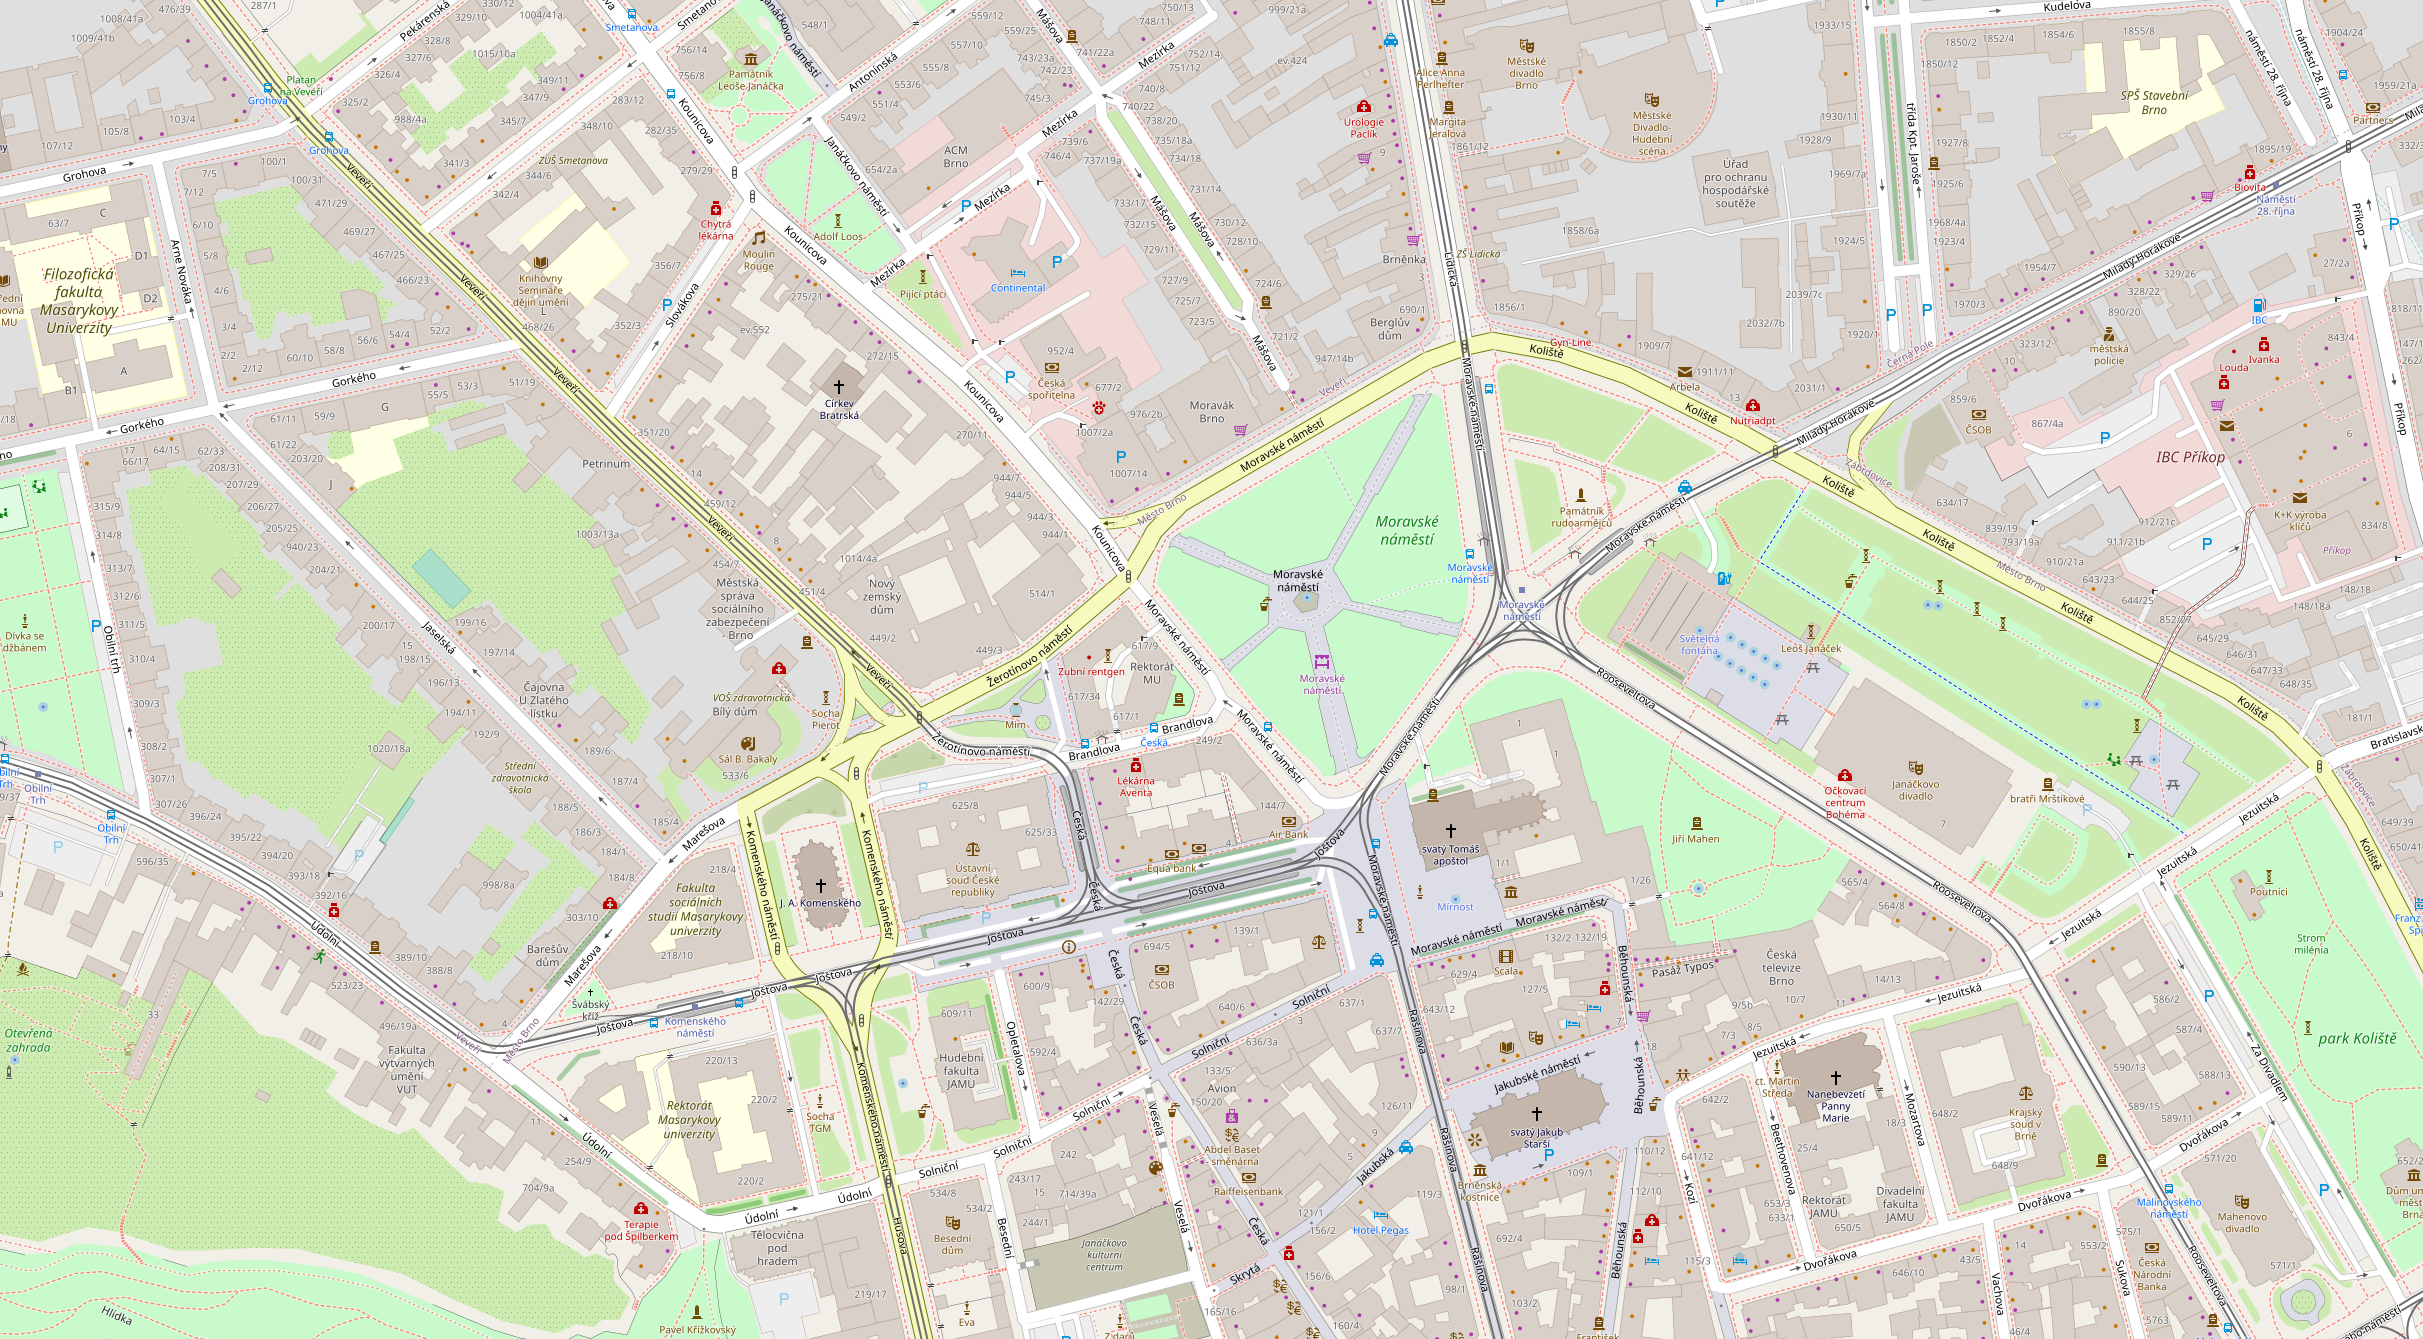
\includegraphics[width=\linewidth]{obrazky-figures/openstreetmap.png}
    \caption{\textbf{OpenStreetMap}. Výsek z mapy časti Brna.}
    \label{fig:openstreetmap}
\end{figure}

\subsection{Dátový model OpenStreetMap}
Prvky (anglicky elements) sú základnou stavebnou súčasťou dátového modelu OpenStreetMap slúžiace k popisu reálneho sveta. Medzi základné prvky OpenStreetMap projektu patria uzol, cesta a relácia. Tieto prvky je možné popísať značkami.

\textbf{Uzol\footnote{\url{https://wiki.openstreetmap.org/wiki/Node}}} (anglicky node) označuje konkrétny bod na povrchu Zeme, je určený svojou zemepisnou šírkou a dĺžkou. Skladá sa minimálne z dvojice súradníc a svojho jednoznačného identifikačného čísla (id).

\textbf{Cesta\footnote{\url{https://wiki.openstreetmap.org/wiki/Way}}} (anglicky way) je usporiadaný zoznam 2 až \numprint{2000} uzlov, ktoré definujú lomenú čiaru. Cesta má aspoň jednu značku alebo je vložená do relácie.

\textbf{Relácia\footnote{\url{https://wiki.openstreetmap.org/wiki/Relation}}} (anglicky relation) sa skladá z jednej alebo viacerých značiek a usporiadaného zoznamu jedného alebo viacerých uzlov alebo ciest. Každý prvok relácie je tzv. člen (anglicky member). Používa sa k popisu závislosti medzi rôznymi prvkami. Každý člen relácie môže voliteľne mať nejakú rolu, ktorá popisuje jeho význam v rámci relácie.

\textbf{Značka\footnote{\url{https://wiki.openstreetmap.org/wiki/Tags}}} (anglicky tag) sa skladá z kľúča a hodnoty. Každá značka popisuje určitú vlastnosť dátových prvkov (uzlov, ciest a relácií) alebo sadu zmien. Kľúč popisuje tému, kategóriu alebo typ mapového prvku (napr. cesta \--- \emph{highway} alebo názvy \--- \emph{name}). Hodnota konkretizuje vlastnosť, ktorú všeobecne popisuje kľúč. Napríklad značka \texttt{highway=residential} predstavuje cestu, ktorá vedie obytnou oblasťou.

\begin{figure}[ht]
    \centering
    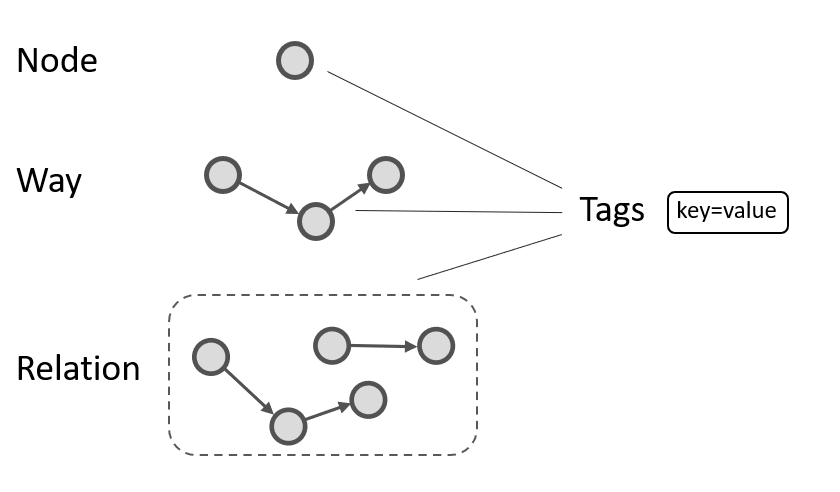
\includegraphics[width=0.64\linewidth]{obrazky-figures/openstreetmap-datamodel.png}
    \caption{\textbf{Dátový model OpenStreetMap}\protect\footnotemark.}
    \label{fig:osmdatamodel}
\end{figure}

\footnotetext{Prevzaté z~\cite{jafari2022building}.}

\section{GIS}
Geografický informačný systém (GIS) je informačný systém, ktorý sa využíva na získavanie, analyzovanie, vizualizáciu a manažment dát s~priestorovým alebo mapovým vyjadrením. GIS spracováva geografické údaje v~digitálnej podobe. Časť takýchto údajov vzniká napr. pomocou satelitných údajov, meraním pomocou polohového systému GPS alebo inými meracími prístrojmi. Údaje v~papierovej podobe je nutné digitalizovať. Súčasťou GIS je hardvér (počítače, servery, zariadenia na zber dát,...), softvér (špecializované programy pre prácu s~priestorovými dátami), dáta (priestorové údaje) a~používatelia (spracovatelia dát, administrátori GIS a~prijímatelia priestorových informácií)~\cite{introductiontogis}. Používatelia systému môžu využívať rôzne metódy spracovania geografických údajov, ktoré umožňujú údaje prehľadávať, triediť, reklasifikovať, transformovať a~modelovať~\cite{hofierka2003gis}.

Geografické dáta v GIS môžu byť organizované dvomi základnými modelmi \--- vektorovým a rastrovým modelom~\cite{holman2014priestorovedata}.

\subsection{Vektorový model}
Vektorový model je nazývaný podľa spôsobu vyjadrenia jeho jednotlivých častí \--- úseky kriviek s definovanou veľkosťou a smerom \--- \emph{vektorom}. Vektorový model pracuje s~tromi variantami objektov:
\begin{itemize}
    \item \textbf{Bod} (point) \--- reprezentuje jednotlivý pár súradníc X, Y. Takýto objekt má príliš malú plochu na to, aby sa dal zobraziť ako plocha (napr. vodopád, vysielač).
    \item \textbf{Línia} (line) \--- reprezentuje množinu usporiadaných bodov \--- uzlov, ktoré sú pospájané do línie. U~takýchto geometrických útvarov je možné vypočítať dĺžku, ale nie je možné zistiť obsah plochy (napr. cesta, rieka).
    \item \textbf{Polygón} (polygon) \--- reprezentuje množinu usporiadaných bodov \--- uzlov, ktoré sú navzájom pospájané líniami do uzatvorenej plochy. U~týchto geometrických útvarov je možné vypočítať obvod a~veľkosť plochy (napr. vodná plocha, lúka).
\end{itemize}

Existujú rôzne modely dát pomocou ktorých je možné reprezentovať geografické objekty s~využitím vektorovej grafiky:
\begin{itemize}
    \item \textbf{Špagetový model} \--- vychádza z postupov využívaných pri digitalizácií máp. Každý objekt na mape je reprezentovaný jedným záznamom a je uložený ako reťazec X, Y súradníc. Z tohto modelu nie je možné získať žiadne informácie o vzťahoch medzi jednotlivými subjektami aj keď sa jedná o priestorové dáta.
    \item \textbf{Topologický model} \--- každá línia tohto modelu začína a končí v uzlu. Všetky informácie tohto modelu sú ukladané do tzv. \emph{topologických tabuliek} \--- tabuľka spojov, súradníc a polygónov. Model vďaka tomu uchováva priestorové vzťahy medzi objektami.
    \item \textbf{Hierarchický model} \--- ukladá zvlášť informáciu o bodoch, líniách a plochách v~hierarchickej štruktúre pre jednoduchšie vyhľadávanie v dátach. V modeli sú takisto zahrnuté aj odkazy medzi jednotlivými druhmi objektov a obsahuje topologickú informáciu. Tento model je pre manipuláciu a vyhľadávanie v dátach najvhodnejší.
\end{itemize}

\subsubsection{Vektorové formáty dát}
Medzi najznámejšie vektorové formáty dát patrí formát \emph{shapefile} vytvorený spoločnosťou ESRI. Tento formát sa ukladá do zariadenia ako skupina aspoň troch súborov, ktoré síce majú rovnaký názov, ale majú rôznu príponu:
\begin{itemize}
    \item hlavný súbor \texttt{*.shp} \--- obsahuje popis geometrie každého záznamu
    \item indexový súbor \texttt{*.shx} \--- prepája prvok v hlavnom súbore so záznamom v atribútovej tabuľke
    \item databázový súbor \texttt{*.dbf} \--- databázový súbor, obsahuje dáta atribútov pre každý záznam
\end{itemize}

Okrem hore zmienených súboroch môže mať \emph{shapefile} aj iné súbory, ktoré obsahujú ďalšie informácie o dátach:
\begin{itemize}
    \item projekčný súbor \texttt{*.prj} \--- ukladá informácie o súradnicovom systéme
    \item priestorové indexy \texttt{*.gix}, \texttt{*.sbn}, \texttt{*.sbx} \--- umožňujú rýchlejšie vyhľadávanie prvkov
    \item atribútové indexy \texttt{*.atx} \--- urýchľujú vyhľadávanie v atribútovej tabuľke
    \item metadátový súbor \texttt{*.shp.xml} \--- metadáta o zvolenom prvku
    \item kódovací súbor \texttt{*.cpg} \--- súbor pre správnu identifikáciu znakov
\end{itemize}

Existuje veľa iných vektorových formátov dát, ktoré sa používajú v GIS ako napr. \emph{KML}, \emph{KMZ}, \emph{GPX} a \emph{GeoJSON}

\textbf{KML} (Keyhole Markup Language) je dátový formát vyvinutý pre aplikáciu Google Earth. Okrem ukladania informácii o geometrii obsahuje možnosti konfigurácie pre Google Earth mapy.

\textbf{KMZ} (Keyhole Markup Zipped) je dátový formát, ktorý sa takisto používa v aplikáciách Google. Tento formát je rozšírením KML formátu, pretože obsahuje okrem textového popisu aj obrázky tvoriace 3D vizualizácie prvku.

\textbf{GPX} (GPS Exchange Format) je formát údajov GPS pre ukladanie bodov, trás a ich atribútov. Ukladá informácie pomocou textu, podobne ako súbory typu KML.

\textbf{GeoJSON}~\cite{rfc7946} je formát založený na formáte JSON (Javascript Object Notation\footnote{\url{https://www.json.org}}). Tento formát je navrhnutý pre reprezentáciu jednoduchých priestorových geografických dát a ich atribútov. Pomocou tohto formátu je možné reprezentovať nasledujúce geometrické typy: \emph{Point}, \emph{LineString}, \emph{Polygon}, \emph{MultiPoint}, \emph{MultiLineString} a \emph{MultiPolygon}. Vo výpise~\ref{lst:geojson} je možné vidieť, ako je reprezentovaný bod (Point) vo formáte GeoJSON.

\lstset{
    caption={\texttt{FeatureCollection} obsahuje vo vlastnosti \texttt{features} objekt typu \texttt{Feature}, ktorý v \texttt{properties} obsahuje informácie viazané na objekt \texttt{geometry}.},
    label={lst:geojson},
    basicstyle=\ttfamily\footnotesize\bfseries,
    xleftmargin=.2\textwidth, xrightmargin=.2\textwidth
}
\begin{lstlisting}
{
  "type": "FeatureCollection",
  "features": [
    {
      "type": "Feature",
      "properties": {
        "kraj": "Moravsko-sliezsky",
      },
      "geometry": {
        "type": "Point",
        "coordinates": [
          17.60100156068802,
          49.196293610455584
        ]
      }
    }
  ]
}
\end{lstlisting}

\subsection{Rastrový model}
Rastrová reprezentácia mapových dát sa na rozdiel od vektorovej zameriava na zemský povrch. Používa sa skôr na javy ako je napr. úhrn zrážok či nadmorská výška.

Základným princípom tohto formátu je pokrytie zemského povrchu pravidelnou alebo nepravidelnou sieťou, pričom jednotka tieto siete je \emph{bunka} (pixel, cell). Nepravidelná sieť má výhodu oproti nepravidelnej siete takú, že pomocou nepravidelnej siete je možné jednoduchšie reprezentovať rôzne prechody z roviny na terénnu hranu. Na druhú stranu použitie nepravidelnej siete je výpočtovo a aj algoritmicky náročnejšie. Keďže v tomto modeli neexistujú objekty známe z vektorového modelu GIS, bunky definujú vlastnú hodnotu sledovaného javu v konkrétnej časti priestoru. Hodnota v jednej bunke odpovedá bodu, rada spojených buniek s rovnakou hodnotou odpovedá línii a skupina navzájom susediacich buniek odpovedá ploche.

\begin{figure}[ht]
    \centering
    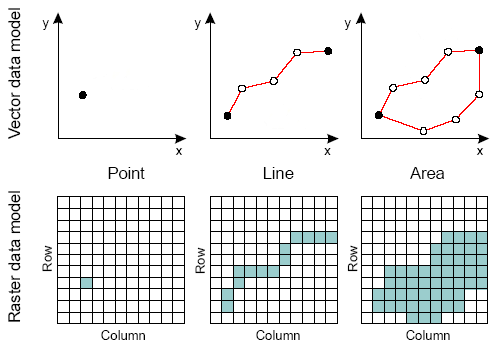
\includegraphics[width=0.5\linewidth]{obrazky-figures/vector-and-raster-data.png}
    \caption{\textbf{Vektorový a rastrový dátový model}\protect\footnotemark.}
    \label{fig:vectorandraster}
\end{figure}

\footnotetext{Prevzaté z~\cite{jukil2017mapdata}}

\subsection{ArcGIS}
V súčasnosti existujú rôznorodé softvéry pre GIS. Medzi najznámejšie patrí ArcGIS od~spoločnosti ESRI, ktorý slúži na mapovanie a priestorovú analýzu navrhnutý tak, aby podporoval poslanie a obchodné ciele organizácií. Tento systém poskytuje tri úrovne licencií. Typ zvolenej licencie rozhoduje o tom, ako sú uložené dáta a ako je možné ich editovať. 

Medzi najznámejšie aplikácie systému ArcGIS patrí ArcMap (použiteľná na priestorové analýzy, editáciu dát a tvorbu kartografických výstupov), ArcCatalog (pomáha organizovať a spravovať všetky dáta), ArcGIS Explorer (volne dostupný prehliadač priestorových dát), ArcGIS for~Server (serverové riešenie pre GIS, umožňuje jednoduchú konfiguráciu webových aplikácií a poskytuje kompletné vývojárske prostredie pre \emph{.NET} a \emph{Java}).

\subsection{ArcČR 500}
ArcČR 500~\cite{arcgis} je digitálna vektorová geografická databáza Českej republiky, spracovaná na úrovni podrobnosti 1 : \numprint{500000}. Obsahom databázy sú prehľadné geografické informácie o~ČR. Zdrojom dát pre geografické dáta ArcČR 500 v 3.3 je databáza Data200, čo je národná vektorová geografická databáza Zeměměřického úřadu (ZÚ) odpovedajúca presnosťou a~stupňom generalizácie 1 : \numprint{200000}. Vstupné dáta z Data200 majú deklarovanú absolútnu presnosť do 100 m. Absolútna polohová odchýlka ArcČR 500 v 3.3 je odhadovaná do 200~m.

Dáta sú uchovávané iba v GIS formátoch firmy ESRI a to vo formáte súborovej databázy. ArcČR 500 je zložená z dvoch geodatabází \--- geografické prvky a administratívne členenie.

\subsubsection*{Geografické prvky}
Geografické prvky boli odvodené zo 17-tich vrstiev databázy Data200. Vrstvy súborovej databázy \texttt{ArcCR500\_v33.gdb} ako aj ich popis a typ prvkov je možné vidieť v tabuľke~\ref{tab:arccr500}.

\begin{table}[H]
\begin{tabular}{|l|p{0.5\linewidth}|l|}
    \hline
    \textbf{vrstva}        & \textbf{popis}                                 & \textbf{typ prvku} \\ \hline
    Letiste                & Letisko                                        & bod                \\
    SidlaBody              & Sídla nad 500 obyvateľov                       & bod                \\
    VyskoveKoty            & Výškové kóty (vrcholy kopcov)                  & bod                \\
    ZeleznicniStanice      & Železničná stanica                             & bod                \\
    Hranice                & Štátna, krajská a okresná hranica              & línia              \\
    Silnice                & Cesta                                          & línia              \\
    VodniToky              & Vodné toky                                     & línia              \\
    Vrstevnice             & Vrstevnice po 25 m                             & línia              \\
    Zeleznice              & Železnice                                      & línia              \\
    BazinyARaseliniste     & Močiar a rašelinisko väčšie ako 30 ha          & polygón            \\
    Lesy                   & Lesné plochy väčšie ako 30 ha                  & polygón            \\
    SidlaPlochy            & Sídla nad \numprint{5000} obyvateľov           & polygón            \\
    VodniPlochy            & Vodné plochy väčšie ako 15 ha                  & polygón            \\
    ChranenaUzemi          & Národné parky a chránené krajinné oblasti      & polygón            \\
    KladyZakladnichMap     & Klady základných máp ČR                        & polygón            \\
    KladyTopografickychMap & Klady vojenských topografických máp            & polygón            \\
    SouradnicovaSitJTSK    & Súradnicová sieť systému JTSK v intervale 1~km & línia              \\
    ZemepisnaSitETRS89     & Zemepisná sieť v systéme ETR89                 & línia              \\
    ZemepisnaSitWGS84      & Zemepisná sieť v systéme WGS84                 & línia              \\
    DigitalniModelReliefu  & Raster digitálneho modelu reliéfu              & raster             \\
    StinovanyRelief        & Raster tieňovaného modelu reliéfu              & raster             \\ \hline
\end{tabular}
\caption{Súborová databáza ArcCR500\_v33.gdb. Prevzaté z~\cite{arcgis} a upravené.}
\label{tab:arccr500}
\end{table}

Každá vrstva tejto databázy môže nadobúdať rôzne hodnoty atribútov, ktoré sú pre danú vrstvu zadefinované. V tejto práci sú uvedené pre ilustráciu iba vrstvy Letisko (tabuľka~\ref{tab:letisko}) a Hranica (tabuľka~\ref{tab:hranica}). V tabuľke \ref{tab:letisko} je možné vidieť, že atribút \texttt{TYP} môže nadobúdať tri hodnoty \--- t.j.~letisko je buď civilné alebo vojenské, alebo civilné a vojenské. Táto vrstva je zobrazená na mape ako bod. Na druhú stranu vrstva \emph{Hranica}, ktorá sa zobrazuje na mape ako línia, nemá takú variabilitu atribútov ako vrstva \emph{Letisko}. V tabuľke~\ref{tab:hranica} je možné vidieť, že daná vrstva má iba jeden zadefinovaný atribút, ktorý ale môže nadobúdať 3 hodnoty \--- t.j. hranica môže byť štátna, krajská alebo okresná.

\begin{table}[H]
    \centering
    \begin{tabular}{|l|l|l|}
    \hline
    \textbf{meno atribútu}         & \textbf{popis}      & \textbf{nadobúdané hodnoty}   \\ \hline
    \textbf{TYP}          & Typ letiska         & \begin{tabular}[c]{@{}l@{}}1 - civilné\\ 2 - vojenské\\ 3 - civilné a vojenské\end{tabular} \\
    \textbf{NAZEV}        & Meno                & \textit{konkrétne meno}       \\
    \textbf{NAZEV\_ASCII} & Meno (ASCII formát) & \textit{konkrétne meno}       \\
    \textbf{ICAO}         & Kód ICAO            & \textit{konkrétny kód}        \\
    \textbf{STATUT}       & Statut letiska      & \begin{tabular}[c]{@{}l@{}}1 - medzinárodné\\ 2 - vnútroštátne\end{tabular}                 \\ \hline
    \end{tabular}
\caption{Vrstva Letisko (Letiste). Prevzaté z~\cite{arcgis} a upravené.}
\label{tab:letisko}
\end{table}

\begin{table}[H]
    \centering
    \begin{tabular}{|l|l|l|}
        \hline
        \textbf{meno atribútu} & \textbf{popis} & \textbf{nadobúdané hodnoty}  \\ \hline
        \textbf{TYP}  & Typ hranice    & \begin{tabular}[c]{@{}l@{}}1 - štátna\\ 2 - krajská\\ 3 - okresná\end{tabular} \\ \hline
    \end{tabular}
    \caption{Vrstva Hranica (Hranice). Prevzaté z~\cite{arcgis} a upravené.}
    \label{tab:hranica}
\end{table}

\subsubsection*{Administratívne členenie}
Dáta z Českého statistického úřadu (ČSÚ) boli použité pre tvorbu dát administratívneho členenia. Vrstvy súborovej geodatabázy \texttt{AdministrativniCleneni\_v13.gdb} ako aj ich popis sa nachádza v tabuľke~\ref{tab:administrativne-clenenie}.
\begin{table}[H]
    \centering
    \begin{tabular}{|lll|}
    \hline
    \textbf{názov}  & \textbf{popis}                 & \textbf{typ prvku} \\ \hline
    \textbf{ZSJ}    & Základné sídelné jednotky      & bod/polygón        \\
    \textbf{UTJ}    & Územné technické jednotky      & bod/polygón        \\
    \textbf{KU}     & Katastrálne územie             & bod/polygón        \\
    \textbf{MOaMC}  & Mestské obvody a mestské časti & bod/polygón        \\
    \textbf{COB}    & Časti obce                     & bod/polygón        \\
    \textbf{OBCE}   & Obce a vojenské újazdy         & bod/polygón        \\
    \textbf{POU}    & Obce s povereným úradom        & bod/polygón        \\
    \textbf{ORP}    & Obce s rozšírenou pôsobnosťou  & bod/polygón        \\
    \textbf{OKRESY} & Okresy                         & bod/polygón        \\
    \textbf{KRAJE}  & Kraje                          & bod/polygón        \\
    \textbf{STAT}   & Štát                           & bod/polygón        \\ \hline
    \end{tabular}
    \caption{Súborová databáza AdministrativniCleneni\_v13.gdb. Prevzaté z~\cite{arcgis} a upravené.}
    \label{tab:administrativne-clenenie}
\end{table}


\section{Kataster}
Kataster predstavuje register resp. zoznam a používa sa vo viacerých významoch:
\begin{itemize}
    \item súpis nehnuteľného majetku, ktorý bol vytvorený pre daňové a úradné účely
    \item kataster nehnuteľností, katastrálna kniha
    \item katastrálne územie
\end{itemize}

\subsection{Kataster nehnuteľností}
Súčasný kataster nehnuteľností~\cite{baudys-katastranemovitosti} na území Českej republiky mal ekvivalent medzi svojimi právnymi predchodcami \--- tzv.~pozemkovú knihu, ktorá slúžila na majetkoprávne účely. Okrem pozemkovej knihy sa používal aj pozemkový kataster, ktorý slúžil na~daňové účely. Pozemkový kataster sa používal približne do roku 1957 a zapisovanie do~pozemkovej knihy bol ukončený v~roku 1964, pretože nevypovedala o~skutočných a~aktuálnych právnych vzťahoch k~nehnuteľnostiam. Preto bola vytvorená nová pozemková evidencia nehnuteľností, ktorej hlavným účelom bolo zaistiť podklady pre plánovanie národného hospodárstva. Táto evidencia bola vedená až do roku 1992, kedy si spoločenské zmeny vyžiadali založenie dnešného katastru nehnuteľností.

Dnešný kataster nehnuteľností plní úlohu pozemkovej knihy aj pozemkového katastru a slúži aj ako podklad pre geografické informačné systémy. Kataster nehnuteľností je definovaný ako súbor údajov o nehnuteľností v Českej republike. Okrem súpisu a popisu nehnuteľností zahŕňa ich geometrické a polohové určenie pre jednu katastrálnu obec alebo katastrálne územie. Aj keď v českom katastri sú zapísané všetky pozemky, zo stavieb sú zapísané v katastri len tie budovy, ktoré stanovuje katastrálny zákon. Ide o budovy s popisným či evidenčným číslom alebo hlavnú budovu v rámci areálu nehnuteľností. Na obrázku~\ref{fig:katastrmapa} je možné vidieť ako vyzerá katastrálna mapa mestskej časti Brno-Královo Pole. Obrázok je exportovaný zo stránky Českého katastru nemovitostí\footnote{\url{https://nahlizenidokn.cuzk.cz/VyberKatastrMapa.aspx}}, ktorý okrem faktických a právnych informácií o nehnuteľnostiach obsahuje katastrálne mapy a informácie o vlastníkoch nehnuteľností.

\begin{figure}[ht]
    \centering
    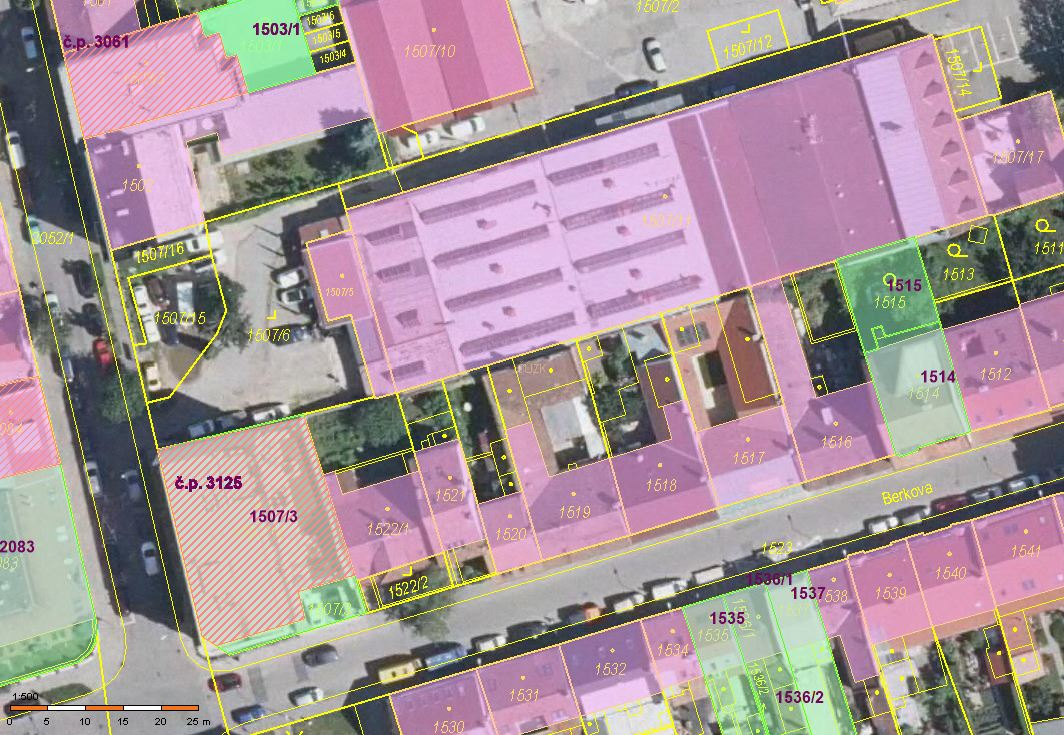
\includegraphics[width=0.8\textwidth]{obrazky-figures/katastr-ortofo-kralovopole.jpg}
    \caption{\textbf{Katastrálna mapa s ortofotomapou mestskej časti Brno-Královo Pole}. Ružová farba predstavuje budovy, budovy so zelenou farbou sú nehnuteľnosti s~cenovými údajmi k~jednotke (byty alebo nebytové priestory), vyšrafované budovy sú nehnuteľnosti s~cenovými údajmi k~parcele.}
    \label{fig:katastrmapa}
\end{figure}

\subsection{Územný plán}
Vlastníci katastrov nehnuteľností si musia byť istý, že na danom území existuje poriadok, ktorý by mal zaručovať, že ich práva nebudú ohrozované náhodnými a~meniacimi sa rozhodnutiami. Územným plánovaním sa predchádza nekoncepčnému a zložitému rozvoja obce. Zaoberá sa všetkými aspektmi nášho prostredia. Ide prevažne o~stavbu sídiel, dopravnú a~ technickú infraštruktúru, ale aj o prvky, ktoré vytvárajú prírodné zložky životného prostredia~\cite{uzemnyplan}.



\chapter{Využité technológie}
\label{technology}
V tejto kapitole sú preberané všetky technológie, ktoré boli použité pri vytváraní užívateľského rozhrania. Ku každej technológií sú napísané dôvody, prečo bola zvolená technológia vhodná na použitie. Aplikácia bola navrhnutá ako klient-server aplikácia, t.j. na strane klienta bolo použité technológie na vizualizáciu výstupov a~na~strane serveru technológie na~spracovávanie dát poslaných od klienta.


\section{GeoPandas}
GeoPandas\footnote{\url{https://geopandas.org/en/stable}} je open-source projekt, ktorý umožňuje jednoduchú manipuláciu geografických dát v jazyku Python. Tento projekt je pokročilejší nástroj umožňujúci načítavanie GIS dát (.geojson, .gdb, .shp, \ldots), manipuláciu s GIS dátami, manipuláciu s~geometrickými útvarmi, prevádzanie súradnicových systémov a vykresľovanie máp. Základnými dátovými štruktúrami projektu GeoPandas sú \texttt{GeoDataFrame} a \texttt{GeoSeries}. Tieto dve dátové štruktúry sú nadstavbou knižnice \emph{Pandas}\footnote{\url{https://pandas.pydata.org}}, pretože rozširujú možnosti dátových štruktúr \texttt{Series} a \texttt{DataFrame} z tejto knižnice. Táto aplikácia je esenciálnou súčasťou celej aplikácie, pretože ju používajú aj iné knižnice.

\texttt{GeoDataFrame} je dvojrozmerná dátová štruktúra, podobná tabuľke s riadkami a~stĺpcami a~je podtriedou \emph{pandas.DataFrame} s pridaným stĺpcom \texttt{geometry} (obrázok~\ref{fig:dataframes}).

\texttt{GeoSeries} je jednorozmerná dátová štruktúra, ktorá je podtriedou \emph{pandas.Series} a~umožňuje ukladať geometrické objekty \--- body, čiary, polygóny, prípadne ich násobné varianty. Predstavuje stĺpec geometry v dátovej štruktúre GeoDataFrame.

\begin{figure}[ht]
    \centering
    \subfloat[\centering \textbf{DataFrame}]{{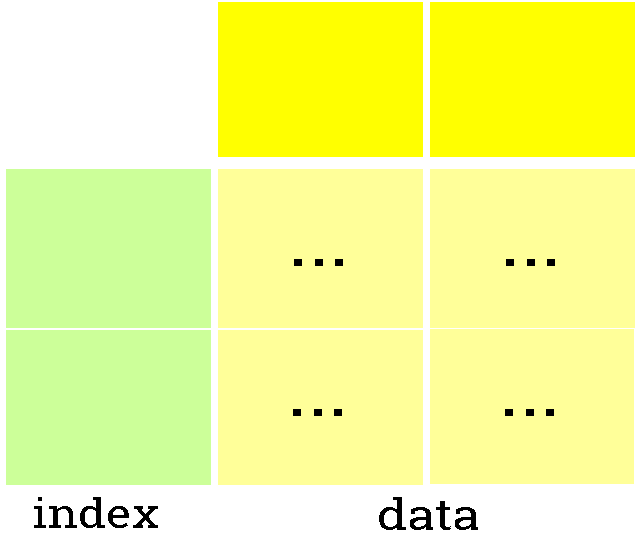
\includegraphics[width=0.25\linewidth]{obrazky-figures/dataframe.pdf}}}
    \qquad
    \subfloat[\centering \textbf{GeoDataFrame}]{{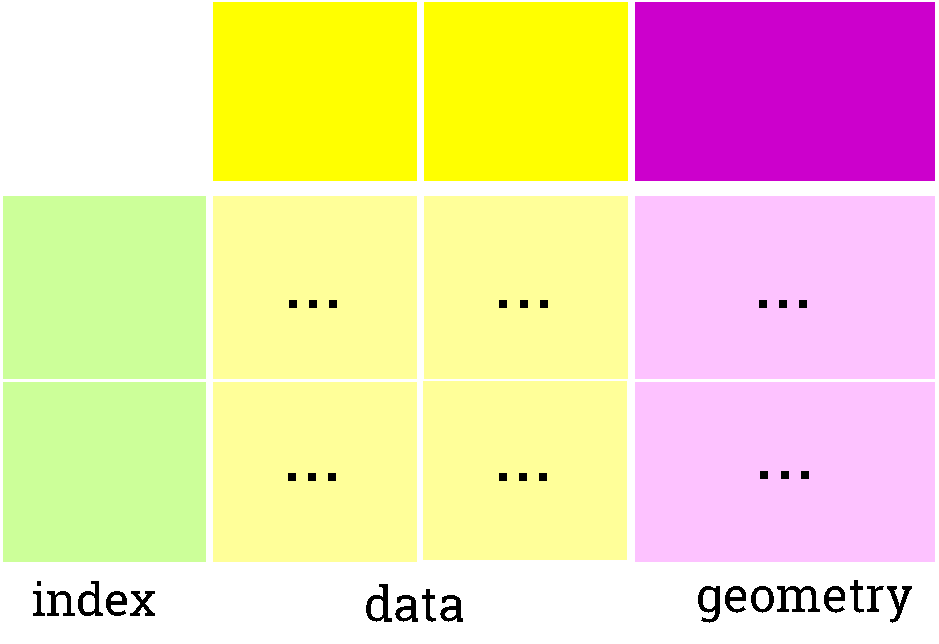
\includegraphics[width=0.31\linewidth]{obrazky-figures/geodataframe.pdf}}}
    \caption{Rozdiel medzi dátovými štruktúrami DataFrame a GeoDataFrame.}
    \label{fig:dataframes}
\end{figure}


\section{OSMnx}
Aby bolo možné pracovať s geografickými dátami, je potrebné ich stiahnuť z určitého zdroja. V~jazyku Python existuje balíček OSMnx\footnote{\url{https://osmnx.readthedocs.io/en/stable}}, ktorý umožňuje sťahovať geopriestorové dáta z~OpenStreetMap. Okrem sťahovania umožňuje tento balíček modelovať, projektovať, zobrazovať a analyzovať pouličné siete reálneho sveta. Balíček OSMnx obsahuje viacero modulov, na túto prácu bol potrebný iba jeden modul \--- modul \texttt{geometries}, ktorý  umožňuje sťahovanie geopriestorových atribútov a entít z OpenStreetMap. Modul sťahuje dáta z OpenStreetMap Nominatim API\footnote{\url{https://nominatim.org}} a vracia dátovú štruktúru GeoDataFrame.


\section{Flask}
Flask\footnote{\url{https://flask.palletsprojects.com/en/2.1.x}} je mikro webový framework napísaný v programovacom jazyku Python. Flask nevyžaduje konkrétne nástroje ani ďalšie vnútorné knižnice. Aj keď sa tento framework považuje za mikro framework, neznamená to, že nie je možné ho rozširovať o rôzne služby~\cite{Oreilly2014Flask}.

Flask som si vybral kvôli jeho jednoduchosti a kvôli tomu, že navrhnutá aplikácia nevyžaduje na prevádzku integráciu s databázovou schémou, ktorú treba integrovať u iných webových frameworkoch. Navyše navrhnutá aplikácia je iba jednostránková aplikácia, takže využívanie robustných webových frameworkov by bolo nepraktické.


\section{Leaflet}
Leaflet\footnote{\url{https://leafletjs.com}} je open-source knižnica v programovacom jazyku JavaScript, používaná na vytváranie mapových webových aplikácii. Táto knižnica je podporovaná na väčšine mobilných a desktopových zariadeniach. Leaflet umožňuje vývojárom jednoducho zobrazovať webové mapy s dlaždicami, získať geopriestorové dáta zo súborov typu GeoJSON, vytvárať interaktívne vrstvy apod.

\subsection{Rozšírenia knižnice}
Okrem základnej funkcionality existujú rôzne rozšírenia, ktoré rozširujú základnú funkcionalitu knižnice Leaflet. V mojej aplikácii sa používajú dve rozšírenia k tejto knižnici: \texttt{Leaflet.heat} a~\texttt{Leaflet.draw}. 

\subsubsection{Rozšírenie Leaflet.heat}
Základom tejto knižnice je knižnica \texttt{simpleheat} z jazyka JavaScript, ktorá sa používa na kreslenie heat máp na plátno. Na vytvorenie vrstvy heat mapy sa používa funkcia \texttt{L.heatLayer(latlngs, options)}, kde:
\begin{itemize}
    \item \texttt{latlngs} \--- predstavuje dvojrozmerné pole, kde každé pole v tomto poli je definované dvojicou (zemepisná dĺžka, zemepisná šírka) resp. trojicou hodnôt (zemepisná dĺžka, zemepisná šírka, intenzita),
    \item \texttt{options} \--- má viacero možnosti, ktoré sa dajú zadefinovať pre danú vrstvu, najdôležitejšie z nich pre moju aplikáciu sú:
    \begin{itemize}
        \item \texttt{max} \--- maximálna intenzita bodu, implicitná hodnota je 1.0
        \item \texttt{radius} \--- rádius každého bodu na heat mape, implicitná hodnota je 25
        \item \texttt{blur} \--- množstvo rozptýlenia, implicitná hodnota je 15
        \item \texttt{gradient} \--- konfigurácia prechodu farieb
    \end{itemize}
\end{itemize}
Na~obrázku~\ref{fig:leafletheat} je možné vidieť ako sa dá pridať tepelná vrstva do mapy a ako daná vrstva vyzerá na mape.

\lstset{
    caption={},
    label={},
    basicstyle=\ttfamily\footnotesize\bfseries
}
\begin{figure}[ht]
\begin{minipage}{.5\textwidth}
\begin{lstlisting}
var heat = L.heatLayer([
     // lat, lng, intensity
    [49.1784, 16.7772, 0.2],
    [49.1784, 16.7774, 0.4],
    [49.1784, 16.7776, 0.6],
    [49.1784, 16.7778, 0.8],
    [49.1784, 16.7780, 1.0]
], {radius: 30}).addTo(map);
\end{lstlisting}
\end{minipage}
\hfill
\begin{minipage}{.5\linewidth}
    \centering
    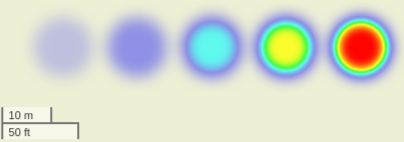
\includegraphics[width=0.7\linewidth]{obrazky-figures/heatlayer-screenshot.png}
\end{minipage}
\caption{\textbf{Rozšírenie Leaflet.heat}. Vľavo sa nachádza implementácia vrstvy, zoradená vzostupne podľa hodnôt intenzít, vpravo sa nachádza zobrazenie týchto bodov na~mape.}
\label{fig:leafletheat}
\end{figure}

\subsubsection{Rozšírenie Leaflet.draw}
Na to, aby užívateľ mohol vybrať určitú oblasť z mapy, na ktorej sa má vykresliť vrstva heat mapy, bolo potrebné použiť rozšírenie Leaflet.draw. Ako je možné vidieť na obrázku~\ref{fig:leafletdraw}, na bočnom paneli mapy v hornom ľavom rohu sa nachádza panel nástrojov, ktorý umožňuje kresliť geometrické útvary na mapu a následne ich upravovať alebo aj vymazávať. Pre~jednoduchosť aplikácie na vybratie určitej oblasti pomocou geometrických tvarov bol použitý iba jeden geometrický tvar \--- obdĺžnik.

\begin{figure}[ht]
    \centering
    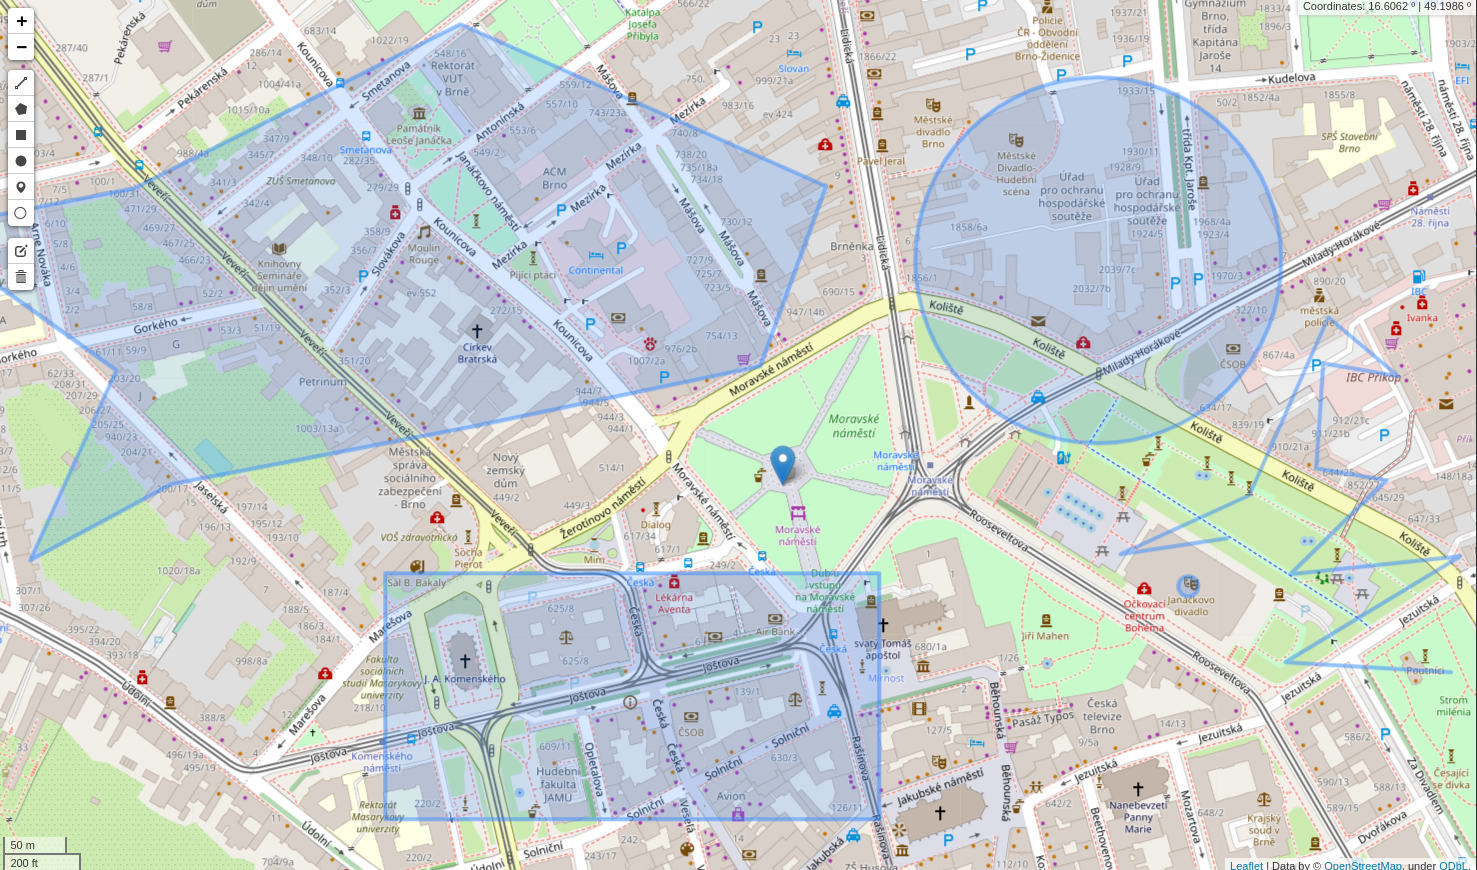
\includegraphics[width=0.8\textwidth]{obrazky-figures/leaflet-draw-screenshot.png}
    \caption{\textbf{Rozšírenie Leaflet.draw} pridáva možnosť kreslenia geometrických útvarov na~mapu \-- krivky, polygóny, obdĺžniky, kruhy, značky a~kruhové značky. Okrem toho je možné pomocou tohto rozšírenia upravovať, presúvať a vymazávať geometrické útvary.}
    \label{fig:leafletdraw}
\end{figure}

\section{HTML}
Jazyk HTML\footnote{HyperText Markup Language, v preklade \emph{Hypertextový značkovací jazyk}.} je jazyk určený na vytváranie webových stránok. Ako už názov napovedá, slovo \emph{hypertextový} naznačuje možnosť odkazov jednotlivých stránok na ostatné. Slovo \emph{značkovací} v spojitosti s jazykmi predstavuje jazyky, ktoré doplňujú text o tzv. \emph{značky} resp.~\emph{tagy}. Všetky značky majú svoje atribúty, ktoré upresňujú jej parametre. Jednotlivé značky je možné do seba vnárať a~spolu tak vytvárajú hierarchickú štruktúru~\cite{kosek1998html}.


\section{CSS}
Štruktúru webových stránok je možné vytvoriť použitím len jazyka HTML, ale na to, aby stránky vyzerali užívateľsky prívetivo, je nutné použiť aj iné nástroje, ktoré pôsobia na~užívateľa prívetivejším dojmom. Preto vznikol mechanizmus \emph{CSS}\footnotetext{Cascading Style Sheets} na vizuálne formátovanie webových stránok. Tento mechanizmus slúži na popis kaskádových štýlov HTML dokumentu.


\section{JQuery}
JQuery\footnote{\url{https://jquery.com}} je rýchla a cross-browser\footnote{Cross-browser kompatibilita je schopnosť webových stránok fungovať v rôznych prehliadačoch.} knižnica z jazyka JavaScript. Zjednodušuje prechádzanie dokumentov HTML, výber DOM\footnote{Document Object Model} elementov, kontrolu udalostí alebo aj vytváranie animácií. Výhodou tejto knižnice je, že je jednoduchou knižnicou na vývoj webových aplikácií. Oproti iným knižniciam v JavaScripte nevyžaduje lepšiu skúsenosť s jazykom JavaScript. Táto knižnica umožňuje okrem už zmienených možností, jednoduchšiu obsluhu \texttt{AJAX} volaní.


\section{AJAX}
Technológia AJAX\footnote{Asynchronous JavaScript and XML} umožňuje meniť obsah stránok bez potreby kompletného načítania zo~servera. Keďže protokol HTTP je bezstavový, akékoľvek stavové informácie je nutné posielať pri každom požiadavku servera a opačne. AJAX nám umožňuje sa takémuto postupu vyhnúť~\cite{lacko2008ajax}. Ako je možné poznať z názvu, AJAX je kombinácia viacerých prvkov:
\begin{itemize}
    \item HTML a CSS na prezentovanie informácií,
    \item DOM na zobrazenie prezentovaných informácií,
    \item metóda na výmenu dát medzi prehliadačom a serverom (napr. XMLHttpRequest objekt),
    \item formát dát posielaný medzi prehliadačom a serverom (napr. XML)
\end{itemize}

V mojej aplikácií som použil AJAX technológiu na aktualizáciu súradníc pri zmene veľkosti alebo presune oblasti určenej na vytvorenie heat mapy.


\section{Bootstrap}
Bootstrap je sada nástrojov, ktorá obsahuje rozšírenie pre jazyky HTML, CSS a JavaScript. Umožňuje vytvárať pomocou veľkého množstva rôznorodých komponentov interaktívne webové stránky. Vyžaduje určitú znalosť HTML a~CSS, pretože väčšinu komponentov je možné vkladať iba pomocou HTML a CSS~\cite{bootstrap}.

V mojej aplikácií používam tzv. \emph{Alert} komponentu t.j. výstražnú správu. Ak sa nepodarila vytvoriť heat mapa z~parametrov poslaných na server, server pošle správu užívateľovi, že heat mapa sa pre zadanú oblasť nepodarila vytvoriť.



% \chapter{Návrh}
% \label{navrh}
% \todo{TODO}
% \blindtext[2]

% \Blindtext


% \chapter{Implementácia}
% \label{implementacia}
% \todo{TODO}

% \blindtext[13]


% \chapter{Testovanie}
% \label{testovanie}
% \todo{TODO}

% \blindtext[1]

% \blindtext[10]



% \chapter{Záver}
% \label{zaver}
% \todo{TODO}

% \blindtext[3]

  \fi
  
  % Kompilace po částech (viz výše, nutno odkomentovat)
  % Compilation piecewise (see above, it is necessary to uncomment it)
  %\subfile{projekt-01-uvod-introduction}
  % ...
  %\subfile{chapters/projekt-05-conclusion}


  % Pouzita literatura / Bibliography
  % ----------------------------------------------
\ifslovak
  \makeatletter
  \def\@openbib@code{\addcontentsline{toc}{chapter}{Literatúra}}
  \makeatother
  \bibliographystyle{bib-styles/Pysny/skplain}
\else
  \ifczech
    \makeatletter
    \def\@openbib@code{\addcontentsline{toc}{chapter}{Literatura}}
    \makeatother
    \bibliographystyle{bib-styles/Pysny/czplain}
  \else 
    \makeatletter
    \def\@openbib@code{\addcontentsline{toc}{chapter}{Bibliography}}
    \makeatother
    \bibliographystyle{bib-styles/Pysny/enplain}
  %  \bibliographystyle{alpha}
  \fi
\fi
  \begin{flushleft}
  \bibliography{projekt-20-literatura-bibliography}
  \end{flushleft}

  % vynechani stranky v oboustrannem rezimu
  % Skip the page in the two-sided mode
  \iftwoside
    \cleardoublepage
  \fi

  % Prilohy / Appendices
  % ---------------------------------------------
  \appendix
\ifczech
  \renewcommand{\appendixpagename}{Přílohy}
  \renewcommand{\appendixtocname}{Přílohy}
  \renewcommand{\appendixname}{Příloha}
\fi
\ifslovak
  \renewcommand{\appendixpagename}{Prílohy}
  \renewcommand{\appendixtocname}{Prílohy}
  \renewcommand{\appendixname}{Príloha}
\fi
%  \appendixpage

% vynechani stranky v oboustrannem rezimu
% Skip the page in the two-sided mode
%\iftwoside
%  \cleardoublepage
%\fi
  
\ifslovak
%  \section*{Zoznam príloh}
%  \addcontentsline{toc}{section}{Zoznam príloh}
\else
  \ifczech
%    \section*{Seznam příloh}
%    \addcontentsline{toc}{section}{Seznam příloh}
  \else
%    \section*{List of Appendices}
%    \addcontentsline{toc}{section}{List of Appendices}
  \fi
\fi
  \startcontents[chapters]
  \setlength{\parskip}{0pt} 
  % seznam příloh / list of appendices
  % \printcontents[chapters]{l}{0}{\setcounter{tocdepth}{2}}
  
  \ifODSAZ
    \setlength{\parskip}{0.5\bigskipamount}
  \else
    \setlength{\parskip}{0pt}
  \fi
  
  % vynechani stranky v oboustrannem rezimu
  \iftwoside
    \cleardoublepage
  \fi
  
  % Přílohy / Appendices
  \ifenglish
    % This file should be replaced with your file with an appendices (headings below are examples only)

% Placing of table of contents of the memory media here should be consulted with a supervisor
%\chapter{Contents of the included storage media}

%\chapter{Manual}

%\chapter{Configuration file}

%\chapter{Scheme of RelaxNG configuration file}

%\chapter{Poster}

\chapter{How to use this template}
\label{jak}

This chapter describes individual parts of the template, followed by a brief instructions on how to use it. If you have any questions, comments etc, feel free to email them to \texttt{sablona@fit.vutbr.cz}.

\section*{Template parts description}

Once you extract the template, you will find the following files and directories:
\begin{DESCRIPTION}
  \item [bib-styles] Literature styles (see below). 
  \item [obrazky-figures] Directory for your images. Currently contains \texttt{placeholder.pdf} (a.k.a TODO image -- see below) and image keep-calm.png to demonstrate inserting raster images (you don't submit these images with your thesis). It is advised to use shorter directory name, so that it is only in your chosen language.
  \item [template-fig] Template images (BUT logo).
  \item [fitthesis.cls] Template (design definition).
  \item [Makefile] Makefile used to compile the project, count standard pages etc. (see below).
  \item [projekt-01-kapitoly-chapters-en.tex] File for Your text (replace it's contents).
  \item [projekt-20-literatura-bibliography.bib] Reference list (see below).
  \item [projekt-30-prilohy-appendices-en.tex] File for your appendices (replace it's contents).
  \item [projekt.tex] Main project file -- definitions of formal parts.
\end{DESCRIPTION}

The style of literature in the template is from Ing. Radek Pyšný \cite{Pysny}, whose work was improved by prof. Adam Herout, dr. Jaroslav Dytrych and Mr. Karel Hanák to comply with the norm and support all frequently used types of citations. Its documentation can be found in the appendix

Aside from compilation to PDF, the Makefile also offers additional functions:
\begin{itemize}
  \item rename files (see below),
  \item count standard pages,
  \item run a wave that adds unbreakable spaces,
  \item compress (zip) the result, ready to be sent to your supervisor and checked (make sure that all the files you've added are included, if not, add them manually).
\end{itemize}

Keep in mind that the wave is not perfect. You always need to check whether or not there is something inappropriate at the end of a line manually -- see Online language handbook\footnote{Internetová jazyková příručka \url{http://prirucka.ujc.cas.cz/?id=880}}.

Similar rules apply also in English - see eg. article Run Ragged\footnote{Run Ragged\url{https://24ways.org/2013/run-ragged/}}, according to which there should be no prepositions, dash or short words (2--3 letters) at the end of the lines, the two lines following each other should not end with a comma and line break should not be also in the phrases from 2-3 words.

\paragraph {Pay attention to page numbering!} If the table of contents is 2 pages long and the second page contains only \uv{Enclosures} and \uv{List of enclosures} (but there is no enclosure), the page numbering is changed by 1 (table of contents and contents \uv{mismatch}). The same thing happens if the second or third page contains only \uv{References} and there's a chance that this can occur in other situations too. There are multiple solutions to this (from editing the table of contents, setting the page counter all the way to more sophisticated methods). \textbf{Check the page numbering before you submit your thesis!}

\section*{Recommendations for working with the template}

\begin{enumerate}
  \item \textbf{Make sure you have the latest version of template.} If you have a template from last year, there should be a newer version (updated information, fixed errors etc.) available at the faculty or study advisor web pages.  
  \item \textbf{Choose a language}, that you want to use for your technical report (czech, slovak or english) and consult your supervisor about your choice (unless it was agreed upon in advance). If your language of choice is not czech, set the respective template parameter in file projekt.tex (e.g.: \verb|document|\verb|class[english]{fitthesis}| and translate the declaration and acknowledgement to english or slovak).
  \item \textbf{Rename the files.} When you extract the files, there should be a file named projekt.tex. If you compile it, it will create a PDF with technical report named projekt.pdf. If multiple students send their supervisor projekt.pdf to have it checked, they have to rename them. For that reason, it is advised to rename the file so that it contains your login and (if needed, abbreviated) work topic. Avoid using spaces, diacritic and special symbols. An appropriate name for your file can look like this: \uv{xlogin00-Cleaning-and-extraction-of-text.tex}. You can use the included Makefile to rename it: 
\begin{verbatim}
make rename NAME=xlogin00-Cleaning-and-extraction-of-text
\end{verbatim}
  \item Fill in the required information in file, that was originally named projekt.text, that means type, year (of submission), thesis title, author's name, department (according to specification), supervisor's titles and name, abstract, keywords and other formal requirements.
  \item Replace the contents of thesis chapters, references and enclosures files with the contents of your technical report. Individual enclosures or thesis chapters can be saved to separate files -- if you choose this approach, it is advised to comply with the file naming convention, and the number will be followed by the chapter title.
  \item If you don't need enclosures, comment the respective part in projekt.tex and erase everything from the corresponding file or delete it. Don't try to come up with an aimless enclosures just to have something in that file. An appropriate enclosure can be the contents of included memory medium.
  \item Delete the chapter and attachment files for a language you haven't used (with or without \texttt{-en}).
  \item Assignment that you download in PDF from FIT IS (link \uv{Thesis assignment}) save to file \texttt{zadani.pdf} and enable its insertion into work by appropriate template parameter (\verb|document|\verb|class[zadani]{fitthesis}|) in \texttt{projekt.tex}.
  \item If you don't want to print references in color (i cannot recommend this without consulting your supervisor), you'll need to create a second PDF for printing and set the template printing parameter:\\ (\verb|document|\verb|class[english,zadani,print]{fitthesis}|). Colored logo must not be printed in black and white.
  \item The binder templace where the thesis will be typeset can be generated in faculty IS at specification. Can be enabled for dissertation using the \tt cover \rm parameter in template.
  \item Don't forget that source files and (both versions) PDF has to be on a CD or other medium included in the technical report.
\end{enumerate}

\subsection*{Instructions for double-sided printing}
\begin{itemize}
\item \textbf{It is advised to consult your supervisor about double-sided printing.}
\item If you used double-sided printing for your thesis and it's thickness is smaller than the thickness of the binder, it doesn't look too good.
\item Enabled using the following template parameter:\\ \verb|\document|\verb|class[twoside]{fitthesis}|
\item After printing a double-sided sheet, make sure that the canon of page construction is in the same position on both pages. Inferior printers with duplex printing unit usually cause a shift by 1--3 mm. This can be solved with some printers. Print the odd pages first, put them back into the same tray and print the even pages.
\item Leave a blank page after title page, table of contents, references, list of tables, list of appendices and other lists to make sure that the following part starts on an odd page (\texttt{\textbackslash cleardoublepage}).
\item Check the final result thoroughly.
\end{itemize}

\subsection*{Paragraph style}

Paragraphs have justified alignment and there are multiple methods for formatting them. In Czech paper literature, a paragraph indentation method is common, where each paragraph of the text have the first line of a paragraph indented by about one to two quads, that is, about two widths of the capital letter M of the base text (always about the same preselected value). In this case, the last line of the previous paragraph and the first line of the following paragraph are not separated by a vertical space. The interleaving between these lines is the same as the interleaving inside the paragraph \cite{fitWeb}.

Another method is indenting paragraphs, which is common for electronic typesetting and for English texts. In this method, the first line of a paragraph is not indented and a vertical space of approximately half of a line is inserted between the paragraphs. Both methods can be used in the thesis, however, the latter method is often more suitable. Methods should not be combined.

One of the above methods is set as the default in the template, the other can be selected by the template parameter \uv{\tt odsaz\rm }.


\subsection*{Useful tools} 
\label{nastroje}

The following list is not a list of all useful tools. If you have experience with a certain tool, feel free to use it. However, if you don't know which tool to choose, consider the ones listed below:

\begin{description}
	\item[\href{http://miktex.org/download}{MikTeX}] \LaTeX{} for Windows -- a distribution with simple installation and great automated package downloading. MikTeX even has it's own editor, but I highly recommend TeXstudio.
	\item[\href{http://texstudio.sourceforge.net/}{TeXstudio}] Portable opensource GUI for \LaTeX{}. Ctrl+click switches between source text and PDF. Integrated spell checker\footnote{Spell checker for czech version can be installed from \url{https://extensions.openoffice.org/de/project/czech-dictionary-pack-ceske-slovniky-cs-cz}}, syntax highlighter etc. To use this tool, you need to first install MikTeX or another \LaTeX{} distribution.
    \item[\href{http://www.winedt.com/}{WinEdt}] A good combination for Windows is WinEdt + MiKTeX. WinEdt is a GUI for Windows, and if you want to use it, you need to first install \href{http://miktex.org/download}{MikTeX} or \href{http://www.tug.org/texlive/}{TeX Live}.
    \item[\href{http://kile.sourceforge.net/}{Kile}] Editor for KDE (Linux) desktop environment. Real-time preview. To use this tool, you need to have \href{http://www.tug.org/texlive/}{TeX Live} and Okular installed.
	\item[\href{http://jabref.sourceforge.net/download.php}{JabRef}] Neat and simple Java program for bibliography (references) file management. No need to learn anything -- provides a simple window and a form for entry editing.
	\item[\href{https://inkscape.org/en/download/}{InkScape}] Portable opensource vector graphic (SVG and PDF) editor. Excellent tool to use to create images for technical text. Difficult to master, but the results are worth it.
	\item[\href{https://git-scm.com/}{GIT}] Great tool for teamwork when it comes to projects, but can be incredibly useful even to a single author. Simple version control system, backup options and transfer between multiple computers.
	\item[\href{http://www.overleaf.com/}{Overleaf}] Online \LaTeX{} tool. A real-time compilation of source text that allows for simple collaboration (supervisor can continuously keep an eye on the progress made), move to a place in source file just by clicking in the PDF preview, spell checker etc. There are some limitations to what you can do if you want to use it for free (some people are comfortable with it for dissertation, others can run into it while they write a~bachelor's thesis) and it is rather slow for long texts. FIT BUT has for students and employees of a license, which can be activated on \url{https://www.overleaf.com/edu/but}.
\end{description}

Note: Overleaf does not use template Makefile -- to get compilation to work, you need to go to the menu and select \tt projekt.tex \rm as s Main document.

\chapter{Writing english texts}
\label{anglicky}
This chapter is taken from web pages of Jan Černocký \cite{CernockyEnglish}.

A lot of people write their technical reports in english (which is good!), but they make a~lot of unnecesary mistakes (which is bad!). I'm not an english export myself, but I've been using this language for a while now to write, read and even communicate -- this chapter contains a handful of important things. If you want to be certain that your thesis or article is 100\,\% correct, your best bet is to hire a native speaker (preferably someone who is technically capable and understands what you write about \ldots).


\section*{In general}

\begin{itemize}
  \item{Before you jump into it head first, I suggest you read a handful of technical articles written in english and try to remember or preferably understand how you should approach writing one yourself.}
  \item{Always use a spell checking tools -- built in tools in Word, or in OpenOffice. If you work on Linux, I suggest you use ISPELL. Some spell checking (I think it's the one in PSPad) are not very good and ignore a lot of mistakes.}
  \item{Use grammer checking tools. I'm not entirely sure if there is one available for Linux, but the one in Word is fairly decent and if it underlines anything with green color, it's probably wrong. You can even copy and paste Latex source code here, fix any and all grammar errors and save it as a clean text again. If you use vim, there's a~built in grammar checking tool too, and it's capable of detecting typos and errors in basic grammar. Write this in the first line of your thesis tex file:
  \begin{verbatim}
    % vim:spelllang=en_us:spell
  \end{verbatim}
  (alternatively \texttt{en\_gb} for OED english) \textit{Editor's note:} There is a very good online tool Grammarly\footnote{\url{https://www.grammarly.com/}}, with free basic version.
  }
  \item{Online dictionaries are good, but don't rely on them in every situation. Usually you get multiple choices and not all of them are correct for the given context.}
  \item{\begin{samepage}You can probably figure out what the correct option is by looking each option up and seeing the context in which they're used, example given: ``advantage/privilege/facility of approach''. Online dictionaries give you a handful of results. Look them up one by one using google search:
  \begin{verbatim}
    "advantage of this approach" 1100000 hits
    "privilege of this approach" 6 hits
    "facility of this approach"  16 hits
  \end{verbatim}
  I'm not saying it's 100\,\% correct, but at least you have something to go on. This can be used to find the correct connectives (e.g. ``among two cases'' or ``between two cases''?)\end{samepage}}
\end{itemize}
       
\section*{SVOMPT and concord}

The structure of an english sentence is SVOPMT: SUBJECT VERB OBJECT MANNER PLACE TIME and there's no other way around it. It is not a flexible structure. There are possibly exceptions in things like a theater play, where something needs to be emphasized. Subject must be present in every single single sentence, people tend to forget as some languages have a sentence structure where the subject can be implicit and not mentioned. SVOMPT applies to dependent clauses too!
\begin{verbatim}
  BAD: We have shown that is faster than the other function. 
  GOOD: We have shown that it is faster than the other function. 
\end{verbatim}

\noindent Concord or grammatical agreement between two words in a sentence -- it sounds silly, but people make countless mistakes here.

\begin{verbatim}
  he has 
  the users have 
  people were 
\end{verbatim}

\section*{Articles}

Articles in english are a nightmare and almost all of us fail to use them correctly. The basic rule is, that if there's a particular noun, it's preceeded by ``the''. Definite articles must be in following phrases:
\begin{verbatim}
  the first, the second, ...
  the last
  the most (superlatives and adverbs) ...
  the whole 
  the following 
  the figure, the table. 
  the left, the right - on the left pannel, from the left to the right ... 
\end{verbatim}

\noindent On the contrary, there can't be an article when you're referring to a specific figure, chapter, etc.
\begin{verbatim}
  in Figure 3.2
  in Chapter 7
  in Table 6.4
\end{verbatim}

\begin{samepage}
\noindent The use of ``a'' and ``an'' is based on the pronounciation, rather than how the word is written:
\begin{verbatim}
  an HMM
  an XML
  a universal model
  a user
\end{verbatim}
\end{samepage}

\section*{Verbs}

Passive voice can be tricky -- regular verbs are usually not a problem, irregular verbs however are a common source of errors, typically
\begin{verbatim}
  packet was sent (rather than send)
  approach was chosen (rather than choosed)
\end{verbatim}
\noindent \ldots most of the time, the spell checker will correct it, but it's not guaranteed.

Tenses are a mess at times. If something just is in general, use present tense. If you did something, use past tense. If you got results that already exist and you just discuss them, use present tense. Try to avoid complicated tenses such as present perfect or worse past perfect if you're not 100\,\% sure.
\begin{verbatim}
  JFA is a technique that works for everyone in speaker recognition. 
  We implemented it according to Kenny's recipe in \cite{Kenny}. 
  12000 segments from NIST SRE 2006 were processed. When compared 
  with a GMM baseline, the results are completely bad. 
\end{verbatim}

\section*{Sentence length and structure}

\begin{itemize}
  \item{Try to write shorter sentences. If you sentence is 5 lines long, it's probably a pain to read, if it can even be done.}
  \item{Comma is a powerful tool and you should use it for your sentence structure. Use a~comma to seperate the initial dependent clause from the main independent clause. Sometimes it is appropriate to put a comma just before ``and'' (unlike other languages)!}
\end{itemize}
\begin{verbatim}
  In this chapter, we will investigate into ... 
  The first technique did not work, the second did not work as well, 
  and the third one also did not work. 
\end{verbatim}

\section*{The specifics of a technical text}

When writing a technical text, don't use common phrases such as
\begin{verbatim}
  he's
  gonna
  Petr's working on ...
\end{verbatim}
\noindent and others. The only tolerated thing is ``doesn't'', but you can never go wrong with ``does not''.

\begin{samepage}
\noindent Technical texts utilize passive voice a lot more than active voice: 
\begin{verbatim}
  BAD: In this chapter, I describe used programming languages. 
  GOOD: In this chapter, used programming languages are described.
\end{verbatim}
\end{samepage}

If you want to use active voice, it's more common to use ``we'', even though you work alone. ``I'', ``my'', etc. are only used when you need to emphasize that you are the person of utmost importance, for example in the conclusion or when discussing ``original claims'' in disertation.


\paragraph{Common erros in words}

\begin{itemize}
  \item{Pay attention to his/hers, it's not ``it's'' but ``its''}
  \item{Image is not picture, it's figure.}
  \item{The connective is ``than'', not ``then'' -- bigger than this, smaller than this \ldots very common error! ``Then'' is used in the context of time.}
\end{itemize}


\chapter{Checklist}
\label{checklist}
This checklist was taken from a template for academic work, that is available on Adam Herout's blog \cite{Herout}, based on the ideas of Igor Szöke\footnote{\url{http://blog.igor.szoke.cz/2017/04/predstartovni-priprava-letu-neni.html}}, with their permission.

A big part of the safety of air transport are checklists. They have checklists for basically anything and everything, even the most cut-and-dry procedures. If a pilot can get over the tedious process of marking off every single checkbox of a procedure, you can as well. Make a checklist of your own before you submit your thesis. \bf Yes, really: \rm print it, grab a pencil and check every single item on the list. It will make your life easier –- avoid unnecessary errors that can be fixed within a couple minutes –- as well as others', at very least your supervisor and reviewer of your thesis.

\subsection*{Structure}
\begin{checklist}
	\item You can tell that the assignment was completed just by looking at the chapter titles as well as their structures.
    \item There is no chapter with less than four pages (except for introduction and conclusion). And if so, I discussed this with my supervisor and they gave me a green light.
\end{checklist}

\subsection*{Figures and charts}
\begin{checklist}
	\item Every single image and table was checked and their position is close to the text that references them. In other words, they’re easy to find.
    \item Every single image and table has a good enough caption, to ensure that the figure makes sense on it’s own, without the necessity to read the text. (There’s no harm in a long caption.)
    \item If an image is taken from somewhere, it is mentioned in the caption: “Taken from [X].”
    \item Texts in all images have a font size similar to the surrounding text (neither signifficantly larger, nor signifficantly smaller).
    \item Charts and schemes are vector graphics (eg. in PDF).
    \item Screenshots don‘t use lossy compression (they‘re in PNG).
    \item All images are referenced in the text.
    \item Axes in charts have their captions (name of the axis, units of measurement, values) and a grind if need be.
\end{checklist}

\subsection*{Equations}
\begin{checklist}
	\item Identifiers and their indexes in equations are single letters (except for rather uncommon cases like $t_{max}$).
    \item Equations are numbered.
    \item All the variables and functions that haven‘t been explained yet are explained below (or rarely above) the equation.
\end{checklist}

\subsection*{Citations}
\begin{checklist}
	\item \bf All used sources are cited. \rm
	\item URL adresses referencing services, projects, sources, github, etc. are referenced using \verb|\footnote{\url{…}}|.
    \item URL adresses in citations are only present, if necessary – article is cited like an article (author, title, where and when was it published), not using URL.
    \item Citations have author, title, publisher (conference title), year of publishing. If a~citation does not have either of these, there is a good explanation for this special case and my supervisor agreed.
    \item If there is anything taken over from some other work in the program source code, it is properly cited therein in conformance with the license.
	\item If an essential part of the source code of the program is taken over, this is mentioned in the text of the thesis and the source is cited.
\end{checklist}

\subsection*{Typography}
\begin{checklist}
	\item No line extends past the right margin.
    \item There is no single-letter preposition at the end of a line (fixed using unbreakable space \verb|~|).
    \item Number of image, table, equation, citation is never a first item of a new line (fixed using unbreakable space \verb|~|).
    \item There is no space before a numeric reference to a footnote (like this\footnote{footnote example}, not like this \footnote{another footnote example}).
\end{checklist}

\subsection*{Language}
\begin{checklist}
	\item I used spellchecker and there were no typos in the text.
    \item I had someone else read my thesis (at least one person), that knows czech / slovak / english well.
    \item Someone who knows english well checked the abstract  in a czech or slovak written abstract thesis.
    \item No part of the text is written in second person (you).
    \item If first person is used (i, we), a subjective matter is being described (i decided, i~designed, i focused on, i found out, etc.).
    \item There are no colloquialisms in the text.
    \item There are no {\it default} words in the text.
\end{checklist}

\subsection*{Result is on a data medium, i.e. software}
\begin{checklist}
	\item I have a non-rewritable data medium ready.
    \begin{itemize}
    	\item CD-R,
        \item DVD-R,
        \item DVD+R in ISO9660 format (with RockRidge and/or Jolliet extension) or UDF,
        \item SD (Secure Digital) card in FAT32 or exFAT format, the card is set to write-protected mode
    \end{itemize}
    \item If the result is online (service, application, …), URL is visible in introduction and conclusion.
    \item The medium contains the following mandatory items:
    \begin{itemize}
    	\item source codes (e.g. Matlab, C/C++, Python, \ldots)
        \item libraries necessary for compilation,
        \item compiled solution,
        \item PDF containing a technical report,
        \item text source code (\LaTeX{}),
    \end{itemize}
    and the following optional items after consulting your supervisor:
    \begin{itemize}
    	\item relevant (e.g. testing) data,
        \item demo video,
        \item poster in PDF
        \item \ldots
    \end{itemize}
    \item Source codes are refactorized, commented and labelled with an authorship header so that others can tell what they actually are.
    \item Any and all snippets of code taken from another sources are properly cited -- differentiated using a opening and in case of multiple lines of code a closing comment. Comments contain everything that the license on web (always try to find out what the license is -- for example, Stack Overflow\footnote{\url{https://stackoverflow.blog/2009/06/25/attribution-required/}} has a very strict citation policy).
\end{checklist}

\subsection*{Submission}
\begin{checklist}
	\item Do I want to delay (by at most 3 years) the publication ? If so, I will submit an application (in IS) at least a month prior to the submission of the academic work, and I'll include attitude of the company that the intellectual property belongs to and needs to be protected.
    \item I have at least minimum number of standard pages (can be calculated using Makefile and by adding number of pages that images translate to). If I'm just under the minimum, I consulted my supervisor about it.
   	\item If I want a two-sided print, I consulted my supervisor about it and I've used correct template settings for two-sided printing. Chapters begin on odd pages.
    \item Technical report is bound in a bookbindery (at least one print, both prints if I'm delaying the publishing).
    \item Title page is followed by the specification (in other words, downloaded from IS and inserted into the template)
    \item Abstract and keywords are uploaded in IS.
      \begin{itemize}
        \item There are no \verb|~| characters for non-breaking spaces in the abstract and keywords in IS.
      \end{itemize}     
    \item PDF of thesis (with clickable links) is in IS.
    \item Both prints are signed.
    \item One (both if I'm delaying the publishing) of the prints contains a data medium with my login written on it using a CD marker (CD marker can be borrowed in library, at Student affairs or when I'm submitting the work).
\end{checklist}

\chapter{\LaTeX{} for beginners}
\label{latex}

This chapter contains commonly used \LaTeX{} packages and commands, that you might need when you're developing a thesis.

\subsection*{Useful packages}

Students usually encounter the same issues. Some of them can be solved using the following \LaTeX{} packages:

\begin{itemize}
  \item \verb|amsmath| -- additional equation typesetting options,
  \item \verb|float, afterpage, placeins| -- image placement,
  \item \verb|fancyvrb, alltt| -- change the properties of Verbatim environment, 
  \item \verb|makecell| -- additional table options,
  \item \verb|pdflscape, rotating| -- rotate a page by 90 degress (for image or table),
  \item \verb|hyphenat| -- change how words break,
  \item \verb|picture, epic, eepic| -- direct image drawing.
\end{itemize}

Some packages are used in this very template (in the lower section of fitthesis.cls file). It is also advised to read the documentation for individual packages.

A table column aligned to left with a fixed width is defined as "L" in the template (used as "p").

To reference a place within text, use command \verb|\ref{label}|. Depending on the placement of this label, it will be a number of chapter, subchapter, image, table or a similar numbered element. If you want to reference a specific page, use command \verb|\pageref{label}|. To cite a literature reference, use command \verb|\cite{identifier}|. To reference an equation, you can use command \verb|\eqref{label}|.

Symbol -- (dash) is used generated using two minus signs (like this: \verb|--|) in \LaTeX.

\subsection*{Commonly used \LaTeX{} commands}
\label{sec:Fragments}

I highly recommend you check the source text of this chapter and see how the following examples are created. The source text even contains helpful comments.

% A left-aligned, fixed-width column is defined in the template as "L" (used as p).

Example table:
\begin{table}[H]
	\vskip6pt
	\caption{Assessment table}
    \vskip6pt
	\centering
	\begin{tabular}{llr}
		\toprule
		\multicolumn{2}{c}{Name} \\
		\cmidrule(r){1-2}
		Name & Surname & Assessment \\
		\midrule
		Jan & Novák & $7.5$ \\
		Petr & Novák & $2$ \\
		\bottomrule
	\end{tabular}
	\label{tab:ExampleTable}
\end{table}

% Ohraničení lze upravit dle potřeby:
% http://latex-community.org/forum/viewtopic.php?f=45&t=24323
% http://tex.stackexchange.com/questions/58163/problem-with-multirow-and-table-cell-borders
% http://tex.stackexchange.com/questions/79369/formatting-table-border-and-text-alignment-in-latex-table

\noindent Example equation:
\begin{equation}
\cos^3 \theta =\frac{1}{4}\cos\theta+\frac{3}{4}\cos 3\theta
\label{rovnice2}
\end{equation}
and two horizontally aligned equations: % znak & řídí zarovnání
\begin{align} \label{eq:soustava}
	3x &= 6y + 12 \\
	x &= 2y + 4 
\end{align}

If you need to reference an equation from the text, you can use command \verb|\eqref|. For example, to reference the equations above \eqref{rovnice2}. If you want to align the equation number vertically, you can use command \texttt{split}:

\begin{equation} \label{eq:soustavaSrovnana}
\begin{split}
	3x &= 6y + 12 \\
	x &= 2y + 4
\end{split}
\end{equation}

Mathematical symbols ($\alpha$) and expressions can be placed even in text $\cos\pi=-1$ and can also be in a footnote%
\footnote{Formula in a footnote: $\cos\pi=-1$}.

Image~\ref{sirokyObrazek} displays a wide image comprised of multiple smaller images. Standard raster image is inserted in the same way as image \ref{keepCalm}.

% Využití \begin{figure*} způsobí, že obrázek zabere celou šířku stránky. Takový obrázek dříve mohl být pouze na začátku stránky, případně na konci s využitím balíčku dblfloatfix (případné [h] se ignorovalo a [H] obrázek odstraní). Nové verze LaTeXu už umí i [h].
\begin{figure*}[h]\centering
  \centering
  
\includegraphics[width=\linewidth,height=1.7in]{obrazky-figures/placeholder.pdf}\\[1pt]
  
\includegraphics[width=0.24\linewidth]{obrazky-figures/placeholder.pdf}\hfill
  
\includegraphics[width=0.24\linewidth]{obrazky-figures/placeholder.pdf}\hfill
  
\includegraphics[width=0.24\linewidth]{obrazky-figures/placeholder.pdf}\hfill
  
\includegraphics[width=0.24\linewidth]{obrazky-figures/placeholder.pdf}
  \caption{\textbf{Wide image.} Image can be comprised of multiple smaller images. If you want to address the partial images from text, use packagae \texttt{subcaption}.}
  \label{sirokyObrazek}
\end{figure*}

% Uncomment this to switch to landscape oriented A3 paper
% \eject \pdfpagewidth=420mm

\begin{figure}[hbt]
	\centering
	
\includegraphics[width=0.3\textwidth]{obrazky-figures/keep-calm.png}
	\caption{Good text is a bad text, that has been changed countless times. You have to start somewhere.}
	\label{keepCalm}
\end{figure}

Sometimes it is necessary to attach a diagram that does not fit on an A4 page. Then it is possible to insert one A3 page and fold it into the thesis (so-called Engineering fold, similar to Z-fold, where two folds are created -- face down and face up). Switching is performed as follows: \texttt{\textbackslash{}eject \textbackslash{}pdfpagewidth=420mm} (210mm to switch it back).

Other frequently used commands can be found above in the text, because a single practical example of correct use is better than ten pages of examples.

% Uncomment this to switch back to A4
% \eject \pdfpagewidth=210mm


% newline command
\newcommand{\odradkovani}{\\[0.3em]}

\chapter{Examples of bibliographic citations}
\label{priloha-priklady-citaci}
The czplain style is based on the style created by mr. Pyšný \cite{Pysny}. This appendix contains a set of supported type of citations with specific examples of bibliograhpic citations.

The next pages of the appendix contain examples of bibliographic citations of the following pubplications and their parts:
\begin{itemize}
   \item Article in a periodical literature (magazine) (str. \pageref{pr-casopis-clanek}),
   \item monographic publication (str. \pageref{pr-monografie}),
   \item conference proceedings (str. \pageref{pr-sbornik}),
   \item conference proceedings entry or book chapter (str. \pageref{pr-kapitola}),
   \item manual, documentation, technical report and unpublished materials (str. \pageref{pr-manual}),
   \item academic work (str. \pageref{pr-thesis}),
   \item web page (str. \pageref{pr-webpage}),
   \item and web site (str. \pageref{pr-website}).
\end{itemize}

\noindent Items are color-coded depending on whether or not they are required or optional:
\begin{itemize}
    \item required element according to the standard
    \item \textcolor{blue}{optional element according to the standard}
    \item \textcolor{magenta}{required element for online information sources according to the standard}
    \item \textcolor{red}{element that is not specified in the standard, but is available and optional within the template's bibliographic style}
\end{itemize}
Required items are only stated if they exist.

\newpage
The bibliography file contains records in the following form:
\begin{verbatim}
@Article{Doe:2020,
   author               = "Doe, John",
   title                = "How to cite",
   subtitle             = "Article citation",
   journal              = "Writing theses and dissertations",
   journalsubtitle      = "Formal aspects",
   howpublished         = "online",
   address              = "Brno",
   publisher            = "Brno University of Technology, 
                          Faculty of information technology",
   contributory         = "Translated by Jan NOVÁK",
   edition              = "1",
   version              = "version 1.0",
   month                = 2,
   year                 = "2020",
   revised              = "revised 12. 2. 2020",
   volume               = "4",
   number               = "24",
   pages                = "8--21",
   cited                = "2020-02-12",
   doi                  = "10.1000/BC1.0",
   issn                 = "1234-5678",
   note                 = "This a made up citation",
   url                  = "https://merlin.fit.vutbr.cz"
}
\end{verbatim}


%-------------------------------------------------------------------------------
\newpage
\section*{Article in a periodical literature - @Article}
\label{pr-casopis-clanek}
\noindent \textbf{Record items}

\medskip

\begin{tabularx}{\linewidth}{X X X}
    Element & BibTeX item & Example\\\hline
    Author & author & Doe, John\\
    Article title & title & How to cite\\
    \textcolor{blue}{Article subtitle} & \textcolor{blue}{subtitle} & \textcolor{blue}{Article citation}\\
    Periodical literature title & journal & Writing theses and dissertations\\
    \textcolor{blue}{Periodical literature subtitle} & \textcolor{blue}{journalsubtitle} & \textcolor{blue}{Formal aspects}\\
    \textcolor{magenta}{Type of medium} & \textcolor{magenta}{howpublished} & \textcolor{magenta}{online}\\
    Edition & edition & 1\\
    Version & version & version 1.0\\
    \textcolor{blue}{Secondary author(s)} & \textcolor{blue}{contributory} & \textcolor{blue}{Translated by Jan NOVÁK}\\
    Place of publication & address & Brno\\
    Publisher & publisher & Brno University of Technology, Faculty of information technology\\
    Month & month & 2\\
    Year & year & 2020\\
    Volume & volume & 4\\
    Number & number & 24\\
    Pages & pages & 8-21\\
    Revision & revised & revised 12. 2. 2020\\
    \textcolor{magenta}{Date of citation} & \textcolor{magenta}{cited} & \textcolor{magenta}{2020-02-12}\\
    Series title & series & Guidelines for writing theses and dissertations\\
    Number in series & editionnumber & 42\\
    \textcolor{magenta}{Digital object identifier} & \textcolor{magenta}{doi} & \textcolor{magenta}{10.1000/BC1.0}\\
    Standard number & issn & 1234-5678\\
    \textcolor{red}{Notes} & \textcolor{red}{note} & \textcolor{red}{This is a made up citation}\\
    \textcolor{magenta}{Availability} & \textcolor{magenta}{url} & \textcolor{magenta}{https://merlin.fit.vutbr.cz}
\end{tabularx}

\bigskip

\noindent \textbf{Bibliographic citation}

\medskip

\noindent \textsc{Doe}, J. How to cite: Article citation. \textit{Writing theses and dissertations: Formal aspects} [online]. 1st ed., version 1.0. Translated by Jan NOVÁK. Brno: Brno University of Technology, Faculty of information technology. February 2020, vol. 4, num. 24, p. 8–21, revised 12. 2. 2020, [cit. 2020-02-12]. Guidelines for writing theses and dissertations, no. 42. DOI: 10.1000/BC1.0. ISSN 1234-5678. This is a made up citation. Available at: \url{https://merlin.fit.vutbr.cz}

%-------------------------------------------------------------------------------
\newpage
\section*{Monographic publication - @Book, @Booklet (book, brochure)}
\label{pr-monografie}
\noindent \textbf{Record items}

\medskip

\begin{tabularx}{\linewidth}{X X X}
    Element & BibTeX item & Example\\\hline
    Author & author & John von Doe\\
    Title & title & How to cite\\
    \textcolor{blue}{Subtitle} & \textcolor{blue}{subtitle} & \textcolor{blue}{Monographic publication citation}\\
    \textcolor{magenta}{Type of medium} & \textcolor{magenta}{howpublished} & \textcolor{magenta}{online}\\
    Edition & edition & 1\\
    \textcolor{blue}{Secondary author(s)} & \textcolor{blue}{contributory} & \textcolor{blue}{Translated by Jan NOVÁK}\\
    Place of publication & address & Brno\\
    Publisher & publisher & Brno University of Technology, Faculty of information technology\\
    Month & month & 2\\
    Year & year & 2020\\
    Revision & revision & revised 12. 2. 2020\\
    \textcolor{magenta}{Date of citation} & \textcolor{magenta}{cited} & \textcolor{magenta}{2020-02-12}\\
    \textcolor{red}{Pages} & \textcolor{red}{pages} & \textcolor{red}{220}\\
    Series title & series & Guidelines for writing theses and dissertations\\
    Number in series & editionnumber & 2\\
    Standard number & isbn & 01-234-5678-9\\
    \textcolor{red}{Notes} & \textcolor{red}{note} & \textcolor{red}{This is a made up citation}\\
    \textcolor{magenta}{Availability} & \textcolor{magenta}{url} & \textcolor{magenta}{https://merlin.fit.vutbr.cz}\\
\end{tabularx}

\bigskip

\noindent \textbf{Bibliographic citation}

\medskip

\noindent \textsc{von Doe}, J. \textit{How to cite: Monographic publication citation} [online]. 1st ed. Translated by Jan NOVÁK.
Brno: Brno University of Technology, Faculty of information technology, February 2020, revised 12. 2. 2020 [cit. 2020-02-12]. 220 p. Guidelines for writing theses an dissertations, no. 2. ISBN 01-234-5678-9. This is a made up citation. Available at: \url{https://merlin.fit.vutbr.cz}
%-------------------------------------------------------------------------------
\newpage
\section*{Conference proceedings - @Proceedings}
\label{pr-sbornik}
\noindent \textbf{Record items}

\medskip

\begin{tabularx}{\linewidth}{X X X}
    Element & BibTeX item & Example\\\hline
    \textcolor{red}{Author*} & \textcolor{red}{author} & \textcolor{red}{Čechmánek, Jan}\\
    \textcolor{red}{Editor*} & \textcolor{red}{editor} & \textcolor{red}{Čechmánek, Jan}\\
    Title & title & How to cite\\
    \textcolor{blue}{Subtitle} & \textcolor{blue}{subtitle} & \textcolor{blue}{Conference proceedings citation}\\
    \textcolor{magenta}{Type of medium} & \textcolor{magenta}{howpublished} & \textcolor{magenta}{online}\\
    Edition & edition & 1\\
    \textcolor{blue}{Secondary author(s)} & \textcolor{blue}{contributory} & \textcolor{blue}{Translated by Jan NOVÁK}\\
    Place of publication & address & Brno\\
    Publisher & publisher & Brno University of Technology, Faculty of information technology\\
    Month & month & 2\\
    Year & year & 2020\\
    Volume & volume & 4\\
    Number & number & 24\\
    Pages & pages & 8-21\\
    \textcolor{magenta}{Revision} & \textcolor{magenta}{revised} & \textcolor{magenta}{revised 12. 2. 2020}\\
    \textcolor{magenta}{Date of citation} & \textcolor{magenta}{cited} & \textcolor{magenta}{2020-02-12}\\
    Series title & series & Guidelines for writing theses and dissertations\\
    Number in series & editionnumber & 2\\
    \textcolor{magenta}{Digital object identifier} & \textcolor{magenta}{doi} & \textcolor{magenta}{10.1000/BC1.0}\\
    Standard number & isbn or issn & 01-234-5678-9\\
    \textcolor{red}{Notes} & \textcolor{red}{note} & \textcolor{red}{This is a made up citation}\\
    \textcolor{magenta}{Availability} & \textcolor{magenta}{url} & \textcolor{magenta}{https://merlin.fit.vutbr.cz}
\end{tabularx}
*Either author or editor is stated.

\bigskip

\noindent \textbf{Bibliographic citation}

\medskip

\noindent \textsc{Čechmánek}, J. \textit{How to cite: Conference proceedings citation} [online]. 1st ed. Translated by Jan NOVÁK.
Brno: Brno University of Technology, Faculty of information technology, February 2020, vol. 4, num. 24, p. 8–21, revised 12. 2. 2020 [cit. 2020-02-12]. Guidelines for writing theses and dissertations, no. 2. DOI: 10.1000/BC1.0. ISBN 01-234-5678-9. This is a made up citation. Available at: \url{https://merlin.fit.vutbr.cz}
%-------------------------------------------------------------------------------
\newpage
\section*{Conference proceedings entry or book chapter - @InProceedings, @InCollection, @Conference, @InBook}
\label{pr-kapitola}
\noindent \textbf{Record items}

\medskip

\begin{tabularx}{\linewidth}{X X X}
    Element & BibTeX item & Example\\\hline
    Author & author & John von Doe\\
    Entry title & title & How to cite\\
    \textcolor{blue}{Entry subtitle} & \textcolor{blue}{subtitle} & \textcolor{blue}{Article citation}\\
    Parent document author & editor or organisation & Smith, Peter\\
    Parent document title & booktitle & Conference proceedings on writing theses and dissertations\\
    \textcolor{blue}{Parent document subtitle} & \textcolor{blue}{booksubtitle} & \textcolor{blue}{Formal aspects}\\
    \textcolor{magenta}{Type of medium} & \textcolor{magenta}{howpublished} & \textcolor{magenta}{online}\\
    Edition & edition & 1\\
    Version & version & version 1.0\\
    \textcolor{blue}{Parent document secondary author(s)} & \textcolor{blue}{contributory} & \textcolor{blue}{Translated by Jan NOVÁK}\\
    Place of publication & address & Brno\\
    Publisher & publisher & Brno University of Technology, Faculty of information technology\\
    Month & month & 2\\
    Year & year & 2020\\
    Volume & volume & 4\\
    Number & number & 24\\
    \textcolor{blue}{Chapter} & \textcolor{blue}{chapter} & \textcolor{blue}{5}\\
    Pages & pages & 8-21\\
    Revision & revised & revised 12. 2. 2020\\
    \textcolor{magenta}{Date of citation} & \textcolor{magenta}{cited} & \textcolor{magenta}{2020-02-12}\\
    Series title & series & Guidelines for writing theses and dissertations\\
    Number in series & editionnumber & 2\\
    Standard number & isbn or issn & 1234-5678\\
    \textcolor{red}{Notes} & \textcolor{red}{note} & \textcolor{red}{This is a made up citation}\\
    \textcolor{magenta}{Availability} & \textcolor{magenta}{url} & \textcolor{magenta}{https://merlin.fit.vutbr.cz}\\
\end{tabularx}

\bigskip

\noindent \textbf{Bibliographic citation}

\medskip

\noindent \textsc{Doe}, J. How to cite: Article citation.
In: \textsc{Smith}, P., ed. \textit{Conference proceedings on writing theses and dissertations: Formal aspects} [online]. 1st ed., version 1.0. Translated by Jan NOVÁK. Brno: Brno University of Technology, Faculty of information technology, February 2020, vol. 4, num. 24, chap. 5, p. 8–21, revised 12. 2. 2020 [cit. 2020-02-12]. Guidelines for writing theses and dissertations, no. 2. ISSN 1234-5678. This is a made up citation. Available at: \url{https://merlin.fit.vutbr.cz}
%-------------------------------------------------------------------------------
\newpage
\section*{Manual, documentation, technical report and unpublished materials - @Manual, @TechReport, @Unpublished}
\label{pr-manual}
\noindent \textbf{Record items}

\medskip

\begin{tabularx}{\linewidth}{X X X}
    Element & BibTeX item & Example\\\hline
    Author (person or organisation) & author & Brno University of Technology, Faculty of information technology\\
    Title & title & Manual for writing theses and dissertations\\
    \textcolor{blue}{Subtitle} & \textcolor{blue}{subtitle} & \textcolor{blue}{Manual citation}\\
    \textcolor{magenta}{Type of medium} & \textcolor{magenta}{howpublished} & \textcolor{magenta}{online}\\
    \textcolor{red}{Document type} & \textcolor{red}{type} & \textcolor{red}{User manual}\\
    \textcolor{red}{Document number} & \textcolor{red}{number} & \textcolor{red}{3}\\
    Edition & edition & 1\\
    \textcolor{blue}{Secondary author(s)} & \textcolor{blue}{contributory} & \textcolor{blue}{Edited by Jan NOVÁK}\\
    Place of publication & address & Brno\\
    Organisation or institution & organization or institution & Brno University of Technology, Faculty of information technology\\
    Month & month & 2\\
    Year & year & 2020\\
    Revision & revised & revised 12. 2. 2020\\
    \textcolor{magenta}{Date of citation} & \textcolor{magenta}{cited} & \textcolor{magenta}{2020-02-12}\\
    \textcolor{red}{Pages} & \textcolor{red}{pages} & \textcolor{red}{220}\\   
    \textcolor{red}{Notes} & \textcolor{red}{note} & \textcolor{red}{This is a made up citation}\\
    \textcolor{magenta}{Availability} & \textcolor{magenta}{url} & \textcolor{magenta}{https://merlin.fit.vutbr.cz}\\
\end{tabularx}

\bigskip

\noindent \textbf{Bibliographic citation}

\medskip

\noindent \textsc{Brno University of Technology, Faculty of information technology}. \textit{Manual for writing theses and dissertations: Manual citation} [online]. User manual 3, 1st ed. Edited by Jan NOVÁK.
Brno: Brno University of Technology, Faculty of information technology, February 2020, revised 12. 2. 2020 [cit. 2020-02-12]. 220 p. This is a made up citation. Available at: \url{https://merlin.fit.vutbr.cz}
%-------------------------------------------------------------------------------
\newpage
\section*{Academic work - @BachelorsThesis, @MastersThesis, @PhdThesis, @Thesis}
\label{pr-thesis}
\noindent \textbf{Record items}

\medskip

\begin{tabularx}{\linewidth}{X X X}
    Element & BibTeX item & Example\\\hline
    Author & author & Brno University of Technology, Faculty of information technology\\
    Title & title & BiBTeX style for ČSN ISO 690 and ČSN ISO 690-2\\
    \textcolor{blue}{Subtitle} & \textcolor{blue}{subtitle} & \\
    \textcolor{magenta}{Type of medium} & \textcolor{magenta}{howpublished} & \textcolor{magenta}{online}\\
    \textcolor{red}{Document type} & \textcolor{red}{type} & \textcolor{red}{Dissertation}\\
    Place of publication & address or location & Brno\\
    School & school & Brno University of Technology, Faculty of information technology\\
    Year & year & 2020\\
    \textcolor{magenta}{Date of citation} & \textcolor{magenta}{cited} & \textcolor{magenta}{2020-02-12}\\
    \textcolor{red}{Pages} & \textcolor{red}{pages} & \textcolor{red}{220}\\
    \textcolor{red}{Appendices} & \textcolor{red}{inserts} & \textcolor{red}{20}\\
    Standard number & isbn & 01-234-5678-9\\
    \textcolor{red}{Supervisor} & \textcolor{red}{supervisor} & \textcolor{red}{Dytrych, Jaroslav}\\
    \textcolor{red}{Notes} & \textcolor{red}{note} & \textcolor{red}{This is a made up citation}\\
    \textcolor{magenta}{Availability} & \textcolor{magenta}{url} & \textcolor{magenta}{https://www.fit.vut.cz/study/theses}\\
\end{tabularx}

\bigskip

\noindent \textbf{Bibliographic citation}

\medskip

\noindent \textsc{Novák}, J. \textit{BiBTeX style for ČSN ISO 690 and ČSN ISO 690-2} [online]. Brno, CZ, 2020. [cit. 2020-02-12]. 80 p., 20. p. apps. Dissertation. Brno University of Technology, Faculty of information technology. ISBN 01-2345-678-9. Supervisor \textsc{Dytrych}, J. This is a made up citation. Available at: \url{https://www.fit.vut.cz/study/theses}
%-------------------------------------------------------------------------------
\newpage
\section*{Web page - @Webpage}
\label{pr-webpage}
\noindent \textbf{Record items}

\medskip

\begin{tabularx}{\linewidth}{X X X}
    Element & BibTeX item & Example\\\hline
    Author & author & Nováková, Jana\\
    Page title & secondarytitle & Post citation\\
    Site title & title & Web on writing theses and dissertations\\
    \textcolor{blue}{Site subtitle}  &  \textcolor{blue}{subtitle} & \\
    \textcolor{magenta}{Type of medium} & \textcolor{magenta}{howpublished} & \textcolor{magenta}{online}\\
    \textcolor{blue}{Secondary author(s)} & \textcolor{blue}{contributory} & \textcolor{blue}{Edited by Jan NOVÁK}\\
    \textcolor{red}{Version} & \textcolor{red}{version} & \textcolor{red}{version 1.0}\\
    \textcolor{red}{Place of publication} & \textcolor{red}{address} & \textcolor{red}{Brno}\\
    \textcolor{red}{Publisher} & \textcolor{red}{publisher} & \textcolor{red}{Brno University of Technology, Faculty of information technology}\\
    Day & day & 12\\
    Month & month & 2\\
    Year & year & 2020\\
    \textcolor{blue}{Time of publication} & \textcolor{blue}{time} & \textcolor{blue}{14:00}\\
    Revision & revised & revised 12. 2. 2020\\
    \textcolor{magenta}{Digital object identifier} & \textcolor{magenta}{doi} & \textcolor{magenta}{10.1000/BC1.0}\\
    Standard number & issn & 1234-5678\\
    \textcolor{red}{Notes} & \textcolor{red}{note} & \textcolor{red}{This is a made up citation}\\
    Availability & url & https://merlin.fit.vutbr.cz\\
    Path & path & Home; Art; The art of citation
\end{tabularx}

\bigskip

\noindent \textbf{Bibliograpic citation}

\medskip

\noindent \textsc{Nováková}, J. Post citation. \textit{Web on writing theses and dissertations} [online]. Edited by Jan NOVÁK. version 1.0. Brno: Brno University of Technology, Faculty of information technology, 2. february 1998 14:10. revised 12. 2. 2020 [cit. 2020-02-12]. DOI: 10.1000/BC1.0. ISSN 1234-5678. This is a made up citation. Available at: \url{https://merlin.fit.vutbr.cz} Path: Home; Art; The Art of Citation.
%-------------------------------------------------------------------------------
\newpage
\section*{Web site - @Website}
\label{pr-website}
\noindent \textbf{Record items}

\medskip

\begin{tabularx}{\linewidth}{X X X}
    Element & BibTeX item & Example\\\hline
    Author (person or organisation) & author & Nováková, Jana\\
    Site title & title & Web on writing theses and citations\\
    \textcolor{blue}{Site subtitle} &  \textcolor{blue}{subtitle} & \\
    \textcolor{magenta}{Type of medium} & \textcolor{magenta}{howpublished} & \textcolor{magenta}{online}\\
    \textcolor{blue}{Secondary author(s)} & \textcolor{blue}{contributory} & \textcolor{blue}{Edited by Jan NOVÁK}\\
    \textcolor{red}{Version} & \textcolor{red}{version} & \textcolor{red}{version 1.0}\\
    \textcolor{red}{Place of publication} & \textcolor{red}{address} & \textcolor{red}{Brno}\\
    \textcolor{red}{Publisher} & \textcolor{red}{publisher} & \textcolor{red}{Brno University of Technology, Faculty of information technology}\\
    \textcolor{blue}{Day} & \textcolor{blue}{day} & \textcolor{blue}{12}\\
    \textcolor{blue}{Month} & \textcolor{blue}{month} & \textcolor{blue}{2}\\
    Year & year & 2020\\
    \textcolor{blue}{Time of publication} & \textcolor{blue}{time} & \textcolor{blue}{14:00}\\
    Revision & revised & revised 12. 2. 2020\\
    Date of citation & cited & 2020-02-12\\
    \textcolor{magenta}{Digital object identifier} & \textcolor{magenta}{doi} & \textcolor{magenta}{10.1000/BC1.0}\\
    Standard number & issn & 1234-5678\\
    \textcolor{red}{Notes} & \textcolor{red}{note} & \textcolor{red}{This is a made up citation}\\
    Availability & url & https://merlin.fit.vutbr.cz
\end{tabularx}

\bigskip

\noindent \textbf{Bibliographic citation}

\medskip

\noindent \textsc{Nováková}, J. \textit{Web on writing theses and dissertations} [online]. Edited by Jan NOVÁK. version 1.0. Brno: Brno University of Technology, Faculty of information technology, 2. february 1998 14:10. revised 12. 2. 2020 [cit. 2020-02-12]. DOI: 10.1000/BC1.0. ISSN 1234-5678. This is a made up citation. Available at: \url{https://merlin.fit.vutbr.cz}.
  \else
    % Bakalárska práca
% Prílohy
% Autor: Peter Koprda
% 2021/2022


\chapter{Obsah priloženého pamäťového média}
\todo{TODO}{}
\begin{verbatim}
/
├── app/
│   ├── data/
│   │   ├── static/
│   │   └── tags.json
│   ├── static/
│   │   ├── css/
│   │   └── js/
│   ├── templates/
│   ├── __init__.py
│   ├── osm_map.py
│   └── view.py
├── latex/
├── run.py
├── requirements.txt
└── README.md
\end{verbatim}

  \fi
  
  % Kompilace po částech (viz výše, nutno odkomentovat)
  % Compilation piecewise (see above, it is necessary to uncomment it)
  %\subfile{projekt-30-prilohy-appendices}
  
\end{document}
